\documentclass{BGSU}
% template.tex version 1.3

\usepackage{alltt}
\usepackage{listings}
\usepackage{hyperref}
\usepackage{longtable}
\usepackage{booktabs}
\usepackage{tabulary}
\usepackage{caption}
\usepackage{graphicx}
\usepackage{epstopdf}
\usepackage{times}
\usepackage[inline]{enumitem}
\usepackage[longnamesfirst]{natbib}

\title{TITLE}
\author{Blake A. Sweeney}
\degree{Doctor of Philosophy}
\date{December 2016}
\advisor{Dr. Neocles Leontis}
\gfr{Dr. Howard Casey Cromwell}
\committee{Dr. Raymond Anthony Larsen \\ \\ 
  Dr. George Bullerjahn \\ \\ 
  Dr. Hans Wildschutte}


% % The first level headings need to be centered, unbolded and 12 point size
% \titleformat{\chapter}[hang]% NEW
%     {\fontsize{12}{15}\centering}{\chaptertitlename\ \thechapter}{1em}{}  %\fontsize{<size>}{<line space>}
% \titlespacing{\chapter}{0pt}{5pt}{5pt}
% \titleformat{\section}
%     {\fontsize{12}{15}}{\thesection}{5pt}{}
% \titlespacing{\section}{0pt}{5pt}{5pt}
% \titleformat{\subsection}
%     {\fontsize{12}{15}}{\thesubsection}{5pt}{}
% \titlespacing{\subsection}{0pt}{5pt}{5pt}
% \titleformat{\subsubsection}
%     {\fontsize{12}{15}}{\thesubsection}{5pt}{}
% \titlespacing{\subsubsection}{0pt}{5pt}{5pt}

\begin{document}

\frontmatter

\maketitle 

\begin{abstract}
This dissertation contains two types of work. The first is the creation and
maintenance of our data pipeline. This chapter focuses on the technical work
behind the extension of our pipeline. In general, this work extends our
previous pipeline to import more data as well as standardizing several parts of
the pipeline. As a result, this work provides a framework for future
modifications of the pipeline. This work was driven both by the move from RNA
3D structures being provided in mmCIF format instead of the more limited PDB
format, as well as the need to clean up the previous version of the pipeline.

The second type of work is scientific including my work on creating equivalence
classes for all RNA 3D structures, using these sets to build representative
sets and then how to use these representative sets along with new quality data
to select a set of high quality loops for future analysis. The new work on
equivalence classes and representative sets was driven by the move from PDB to
mmCIF formats. This move forced the redesign of the previous method, as it
would only use the largest chain in each PDB file. This change allowed me
to reconsider the approach and allowed several improvements. 

The work on loop quality was prompted by the release of new structure quality
data, Real Space R Z-Score (RSRZ). This data allows the examination of how well
a proposed structure fits the data it is built from. By using this we can limit
our studies of RNA loops to only those that are from high quality, well modeled
structures. 

% vim ft=markdown

\end{abstract}

\begin{acknowledgments}
Thank you to all those who supported through this. My advisor, my lab, my
family and Lisa. I couldn't have done this without you.

\end{acknowledgments}

\tableofcontents

\listoffigures

\listoftables

\mainmatter % starts over page counter and gives regular page numbers

\chapter{OVERVIEW OF THE RNA.BGSU.EDU DATA PIPELINE, DATABASE AND SUPPORTED
ON-LINE RESOURCES}

In this chapter I will discuss the \href{http://rna.bgsu.edu}{RNA.BGSU.EDU}
pipeline and database. The aim is provide the reader with an overview of the
pipeline and familiarity with concepts and design. This chapter will first
provide a context for my work on the pipeline by discussing the goals, rationale
for this work and the principles defining the design of the pipeline and
database. This will then discuss the scientific value of our pipeline followed
by the design and how it allows us to achieve the principles. Finally we will
provide an overview of the implementation. 

\section{Goals for the BGSU RNA pipeline}

One of the major grant activities in our lab is the development, maintenance and
extension of our data pipeline and database that imports data from new
RNA-containing structure files as they appear in PDB on a weekly basis. The
pipeline is a python and Matlab application that annotates all pairwise
nucleotide interactions, groups structurally similar RNA molecules into
equivalence sets, identifies high quality representative sets of RNA structures
and extracts and clusters RNA 3D motifs and stores all these derived data in a
locally maintained MySQL database.

We have developed these tools to achieve the aims of NIH founded work carried
out in collaboration with with Dr. John Westbrook and Dr. Helen Berman at the
Nucleic Acids Database (NDB). This is the sixth year of the collaboration, which
began in 2010. The aims of the grant are:

\begin{enumerate}
        \item Deepen our understanding of RNA 3D structure by extracting and
                organizing 3D motifs

        \item Improve our understanding of the structure variation of RNA
                molecules and RNA complexes by examining and comparing 3D
                structures assigned to the same sequence/structure "equivalence"
                class.

        \item Accelerate the study of the correspondence between RNA 3D
                structure and RNA sequence

        \item Provide annotations for RNA-protein interactions

        \item Develop new and extended tools for delivery, search and
                visualization of the RNA sequence and structure annotations
                described in Aims 1-4 and make them available in the NDB.
\end{enumerate}

As a part of the grant we provide annotations to NDB on a weekly basis. These
data include our nonredundant sets and associated equivalence sets, nucleotide
interaction annotations, as well as motif clusterings. In the near future we
will add RNA-protein interactions.

The data computed in our pipeline are used to support research resources. We
provide the RNA community with the BGSU RNA site, the RNA 3D motif library,
JAR3D, WebFR3D, R3DAlign, and R3D-2-MSA. As these resources require access to
up-to-date RNA structures, it is essential that the database and pipeline always
produce all the required data.

Secondly, it is essential that the pipeline be easy to maintain, extend and
improve by successive groups of graduate students and research associates. After
the departure of Anton Petrov and during most of my Ph.D. work it has been my
responsibility to maintain and update the pipeline and database. During the time
I was charged with these responsibilities major improvements were made to take
advantage of new mmCIF formats from PDB. The following projects are underway
that will extend the pipeline's capabilities: 
\begin{enumerate*}
        \item Poorna Roy is writing code to annotate nucleotide-amino acid
                interactions, 
        \item Maryam Husseieni is writing code to annotate and extract
                multi-helix functions and cluster them for the RNA 3D Motif
                Atlas, 
        \item Once finalized these results will be written into the database 
        \item We continue on an ongoing basis to improve base-pair annotation
                (Dr. Craig Zirbel), loop extraction (my work) and motif
                clustering.
\end{enumerate*} 
As soon as these new results and functions are tested and validated these
improvements will be integrated into the pipeline's weekly update functions.

Thus the operations goals for our database and pipeline are:
\begin{enumerate}
        \item The pipeline must store only correct data in the database
        \item The pipeline must run reliable each week to maintain current data
        \item The pipeline must be ease to maintain, update and improve
\end{enumerate}

In the next sections I will discuss how the changes I have made to the previous
version help us achieve these goals.

\section{Comparison of the current BGSU RNA pipeline to other resources}

We have evaluated other software options and found them unsuitable for our
current aims. The main resource we considered was the previous implementation by
Dr. Anton Petrov \cite{Petrov2012}. The implementation was a part of his dissertation research.
Much of the previous pipeline was not suitable for our current requirements.

First, the previous version did not work with mmCIF data. In December 2014, the
protein databank (PDB) transitioned from the outdated fixed columnar width  PDB
format to a new mmCIF format for all 3D structure data.

Second, the previous version of the database and pipeline did not work to ensure
the validity of data. Consequently, I discoverd that our database contained
"orphan data". Orphan data is data that is missing related information. For
example, there were structures which had been placed into an NR group, but we
had no information on the resolution. In addition, a careful reading of the code
showed it was possible for the pipeline to write incomplete data. Incomplete
data is when we do not write all annotations for a structure. For example, if
there are 100 annotated base pairs, writing 99 of them would constituent writing
incomplete data. My rewrite was aimed at fixing these issues as well as
usability of the pipeline.

Finally, the previous version did not centralize the core logic of the pipeline
in a module making the pipeline harder to maintain. To explain, all parts of the
pipeline have the same core logic as detailed in a later section. Each part of
the pipeline that computes data is referred to as a ``stage''. The stage is
primarily responsible for computing data, while the core manages ensuring that
the overall pipeline behaves correctly.

A good example of centralizing logic, is the logic for rolling back failed
imports and checking if data has been computed. The previous version had not
centralized this logic so adding new computations required the programmer to add
logic to ensure that these actions happened correctly. In addition, requests to
remote resources were not always retried leading to some requests being more
fragile than others.

Another potential option was to use is the
\href{https://github.com/pharmbio/sciluigi}{sciluigi} which is built off the
luigi package provided by Spotify. Sciluigi package contains a framework for
building pipelines and is being adopted by the bioinformatic community. I have
chosen not to use sciluigi because it was released after I had already written a
large portion of the pipeline. While sciluigi is a well designed framework it
does not offer a compelling reason to rewrite large portions of our existing
framework. Had it existed prior to my start I would have likely used it.

\section{Design requirements for the BGSU RNA pipeline and database}

In more detail, to support the research goals, our pipeline must fulfill the
following requirements.

\begin{enumerate}
        \item The pipeline must always keep the database in a valid state.
        \item The pipeline must operate efficiently and avoid recomputing data unnecessarily
        \item The pipeline should facilitate user control when manual operation is required.
        \item The pipeline must be as reliable as possible.
        \item The pipeline must be designed so additions will respect all constraints.
\end{enumerate}

We will discuss each requirement and the rationale behind each one.

\subsection{Maintaining validity of data}

For a database to remain valid, two properties must be maintained. First, the
database must be complete. This means that the database should not be left in a
state with any partial data for any structure. For example, the database should
not have partial base pair annotations for a given structure: it should have all
or none. This requirement must be respected because our data supports several
sources: equivalence classes of similar structures and the representatives sets
they support and the annotations we provided to NDB
\cite{CoimbatoreNarayanan2014}, also the R3D-2-MSA \cite{Cannone2015}, JAR3D
\cite{Roll2016}, WebFR3D \cite{Petrov2011a}, and R3DAlign \cite{Rahrig2013}
sites all rely on data produced by pipeline in the database.

\subsection{Ensuring the validity of the database}

The second property of a valid database is that it is consistent. Consistency is
best explained through an example. Keeping the database consistent means
preventing situations from arising where we annotate a base pair involving RNA
nucleotide residues that we have not yet created and stored in the database. In
database terms, this requirement is referred to as preventing "orphan data".
Whenever data are inconsistent any analysis or display of the stored data will
fail, for lack of referenent.

By striving to keep the database in a valid and consistent state, we ensure that
the database is always usable for analysis and display on webpages, even when
the pipeline fails to update with new data. Without this it would make our other
tools, such as JAR3D and RNA 3D Hub, unstable. Providing these resources in an
ongoing and stable manner is a major grant activity in the lab, which is why
this is the most important design consideration of the pipeline.

Preventing the writing of incomplete or orphan data is also essential to
avoiding or minimizing the unnecessary recomputation of data. As we learned
during the transition of CIF format files, which required the computation of
most annotations, recomping all data for each each run of the pipeline would
take several weeks. This is too slow and completely unnecessary for our planned
weekly update runs of the pipeline. Thus the pipeline is designed to only
compute data for new structures or manually specified structures that need to be
recomputed for some particular reason, at the manager's discretion.

\subsection{Controlling the pipeline}

The next priority, ease of controlling which stages and structures to run during
manual operation, is intended to facilitate error correction. Work with previous
version of the pipeline showed that extensive manual work was always needed to
rerun the correct stages with the correct data. This manual work was
error-prone, and frequently produced even more problems that need correction. By
automating the repetitive manual work, I succeeded in making it easier to
recover from errors.

\subsection{Pipeline Reliability}

The fourth consideration is that the pipeline must be as reliable as possible.
Reliability means that the pipeline will compute as much data as possible
despite errors. Errors in programs are inevitable and must be anticipated in the
design of the pipeline. Even if all parts of the pipeline are written correctly
it can still fail because of anomalous events generated by external resources.
For example, the pipeline has failed when:  PDB provided incomplete data or when
the network experienced instability during few fractions of a second required to
complete a web request. These and other issues that I have encountered during
the years I was responsible for pipeline operation, convinced me of the high
priority of making the pipeline as robust as possible.

The final consideration is ease of adding new "stages" to provide new
functionality as this will carried out on an ongoing basis by current and new
students involved in the project. They should be able to make changes without
having to know all the details of how the pipeline works, confident that they do
not have to deal with ensuring the validity of the database and the stability of
the pipeline in order to make improvements and additions of new functionality.

\section{Implementation of the BGSU RNA data pipeline}

In this section I discuss the improvements to the pipeline that enable it to
fulfill the design requirements outlined above. These improvements required
coordinated changes to occur both in the pipeline application and the database.
Each requirement in turn.

\subsection{Ensuring data validity}

To maintain validity of data in a database, it is essential to add constraints
to the database. Constraints are requirements on one or more columns that ensure
certain criteria must be met before adding or modifying data in that column. The
constraints I have added include uniqueness constraints and foreign key
constraints as appropriate. Constraints were added to  nearly every table in the
database. These constraints could not be added prior to these improvements
because the database was not configured to allow them.

A uniqueness constraint ensures that no two rows in the same table may have the
same data values in any column. Uniqueness constraints may span more than one
column. For example, I have added a uniqueness constraint on the ``pdb\_id'' and
``chain\_name'' column in the ``chain\_info" table. This table stores information
about all chains and by placing the uniqueness constraint on these two columns I
ensure that there can be no two chains in the same structure with the same
combination of PDB id and chain name. This constraint reflects the logical
structure of the data. By adding these constraints, I ensure that the data in
the database is logically correct as regarding chains.

The second type of constraint I introduced is the consistent implementation of
foreign keys wherever required to allow the many tables in our database to work
together properly. These ensure that entries in one column of one table exist in
another column of another table. These safeguard data completeness. The use of
foreign keys allows the expression of the requirement of ``interactions must be
built from known residues'. To describe a specific example, we have a table
called ``unit\_info'' which contains data for all residues, RNA, DNA, protein,
ligands, etc, known in the database. In the unit\_info table there is a
``unit\_id'' column that provides a unique identifier for all units (i.e.
residues, whether RNA, DNA or protein). The ``unit\_pairs\_interactions'' table
contains all pairwise interactions between RNA residues, such as base pair and
base stacking interactions. It contains a ``unit\_id\_1'' and ``unit\_id\_2'' column
which specify the first and second units forming the interaction. For an
interaction represented by a row in the unit\_pairs\_interactions table to be
valid, the entries in the ``unit\_id\_1'' and ``unit\_id\_2'' must exist  in the
``unit\_id'' column of the ``unit\_info'' table. I have enforced this logical
requirement by declaring that ``unit\_id\_1'' and ``unit\_id\_2'' are foreign keys
link to ``unit\_id'' in the unit\_info table.

At the level of the pipeline application, I ensure data validity by implementing
procedures to automatically rollback failed imports. Because we have foreign key
and uniqueness constraints, it is possible to attempt to write data that will be
rejected. For example, if the pipeline attempts to write an interaction between
units that do not exist, the database will reject the data because of the
foreign key constraints. I rewrote the pipeline so that in the event of such an
error during a data entry operation, all interactions that were written for that
structure will be deleted. This prevents the writing of partial data for any
single structure, ensuring the database remains complete, ie ensuring the
absence of partial data.

\subsection{Minimizing the number of computations}

If the pipeline were to recompute all data on every update a single run would
take at least several weeks to complete with currently available resources.
Given that we are committed to provide weekly updates to NDB, this is
unacceptable. However, the capability to easily force data to be recomputed is
also crucial. For example, we update our classification of pairing interactions
from time to time. When this is done, we must be able to easily update the
entire database with the new pairing annotations. I have implemented the
capability to make such updates by simply telling the pipeline to delete the old
data and recompute the new data.

I have changed the pipeline execution to first check whether data have already
been computed for each input and only computing data when none are present, or
when the user explicitly requests the pipeline to select recompute selected
data. Now as currently configured all parts of the pipeline go through the steps
shown in Figure~\ref{fig:stage-flow}. With this logic I can ensure that only the
required data are computed. The previous version of the pipeline had a similar
capability however my additions make it more comprehensive, as well as, ensuring
that old data are always deleted prior to recomputing existing data. In the
previous version it was not required that all parts have consistent behavior in
the face of existing data. I have centralized the logic for recomputing and
deleting old data.

\begin{figure}
  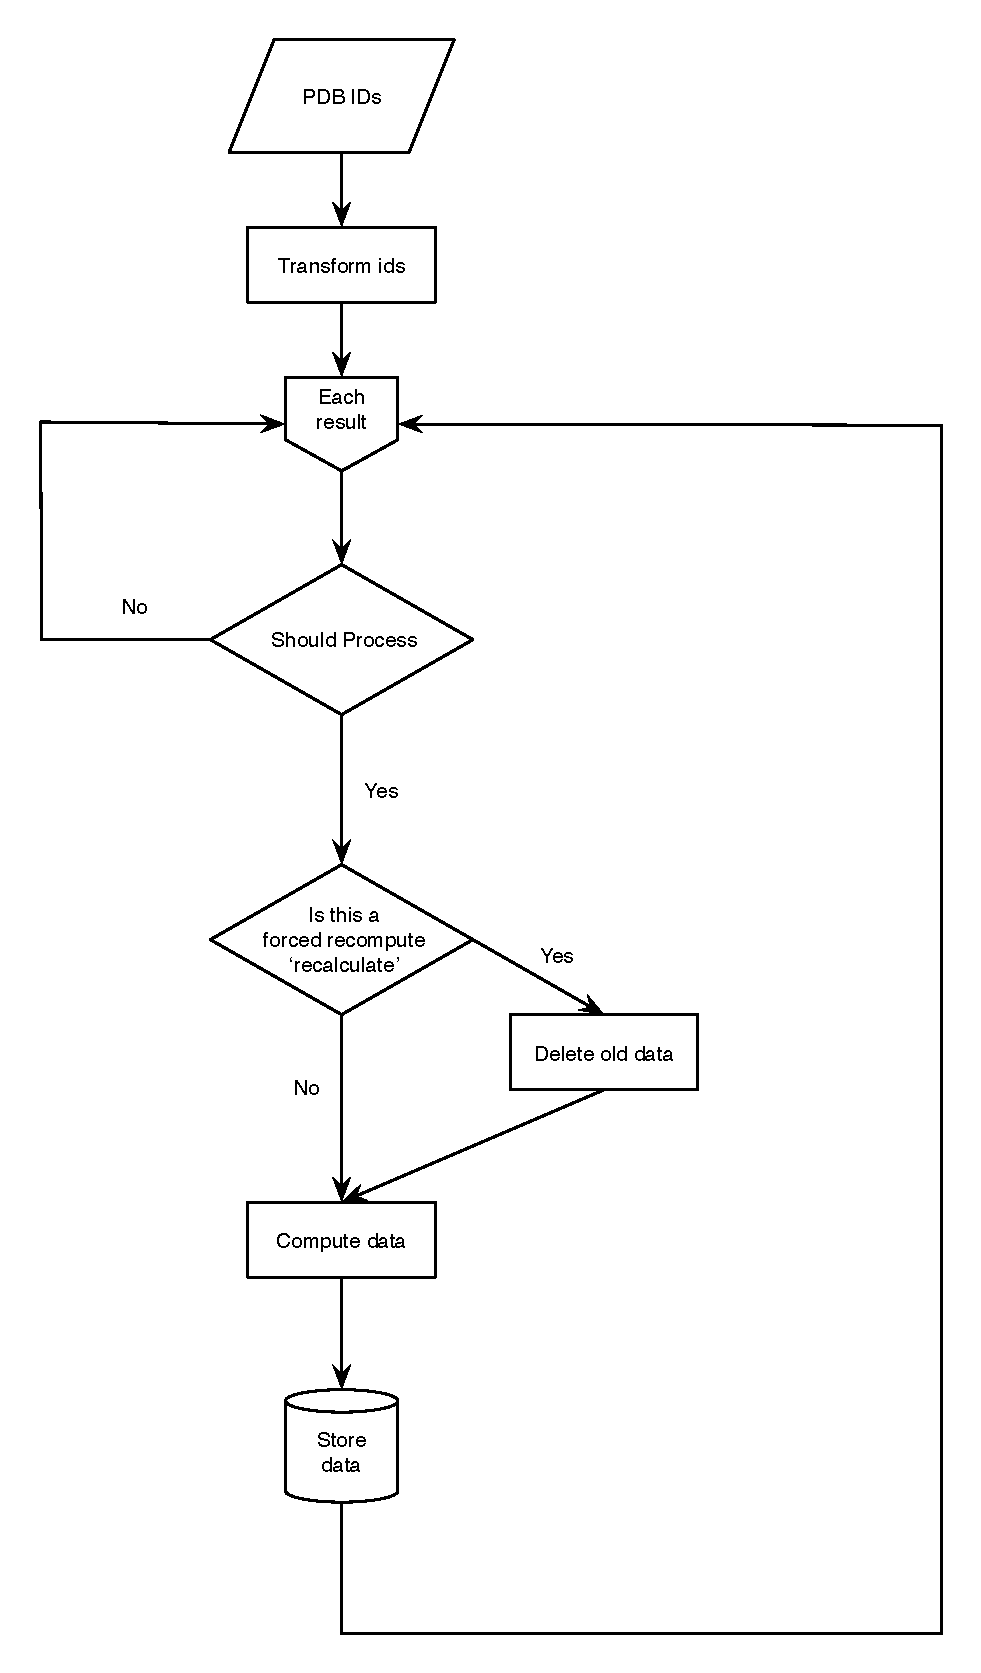
\includegraphics[height=8in]{chapter-2/figs/stage-flow}
\caption{Figure summarizing the logical flow for each stage. This figure shows
the general scheme of all stages.}
\label{fig:stage-flow}
\end{figure}

This requirement ensures efficient execution times of our pipeline. Without it
our weekly, or even monthly update schedule could not be maintained. However, in
order to correctly skip recomputing old data, the database must always be
complete. Should the pipeline begin to save incomplete data, it will never
attempt to recompute and fill in missing data. For this reason, it is essential
that the database always remain complete.

\subsection{Providing control over the data computed}

The day-to-day goal of the pipeline is to run weekly updates using all available
structures. In this case the intent is to compute all annotations for all
structures. However, it is often useful and sometimes necessary to run specific
annotations on specific structures. For example, when testing a new set of
annotations it is desirable to select a few test structures on which to run only
the new annotations, and then examine the results.

To make this possible, I have restructured the pipeline to provide a single
unified point of entry that takes as input the name of the part to run and the
particular structures to analyze, or an option to include all available
structures. In the previous version of the pipeline there were several possible
entry points. The primary entry point was the ``update'' component. This part
would run everything required for a weekly update in the correct order. The
other entry points were specific to individual components such as loading
interactions. This was an issue because parts of the pipeline have dependencies
upon each other. For example, to compute the pairwise interactions, the
structure must first be downloaded. Previously, these dependencies were implicit
in the design of the update component and were not stated explicitly, leading to
potential confusion.

These dependencies are now encoded into the pipeline using a dependency graph as
shown in Figure~\ref{fig:stage-deps}. This graph can be sorted using a topological
sort to produce a linear ordering. I have implemented this logic as part of the
``dispatcher'' which determines which modules to run and in which order to run
them in for a given application.


\begin{figure}
  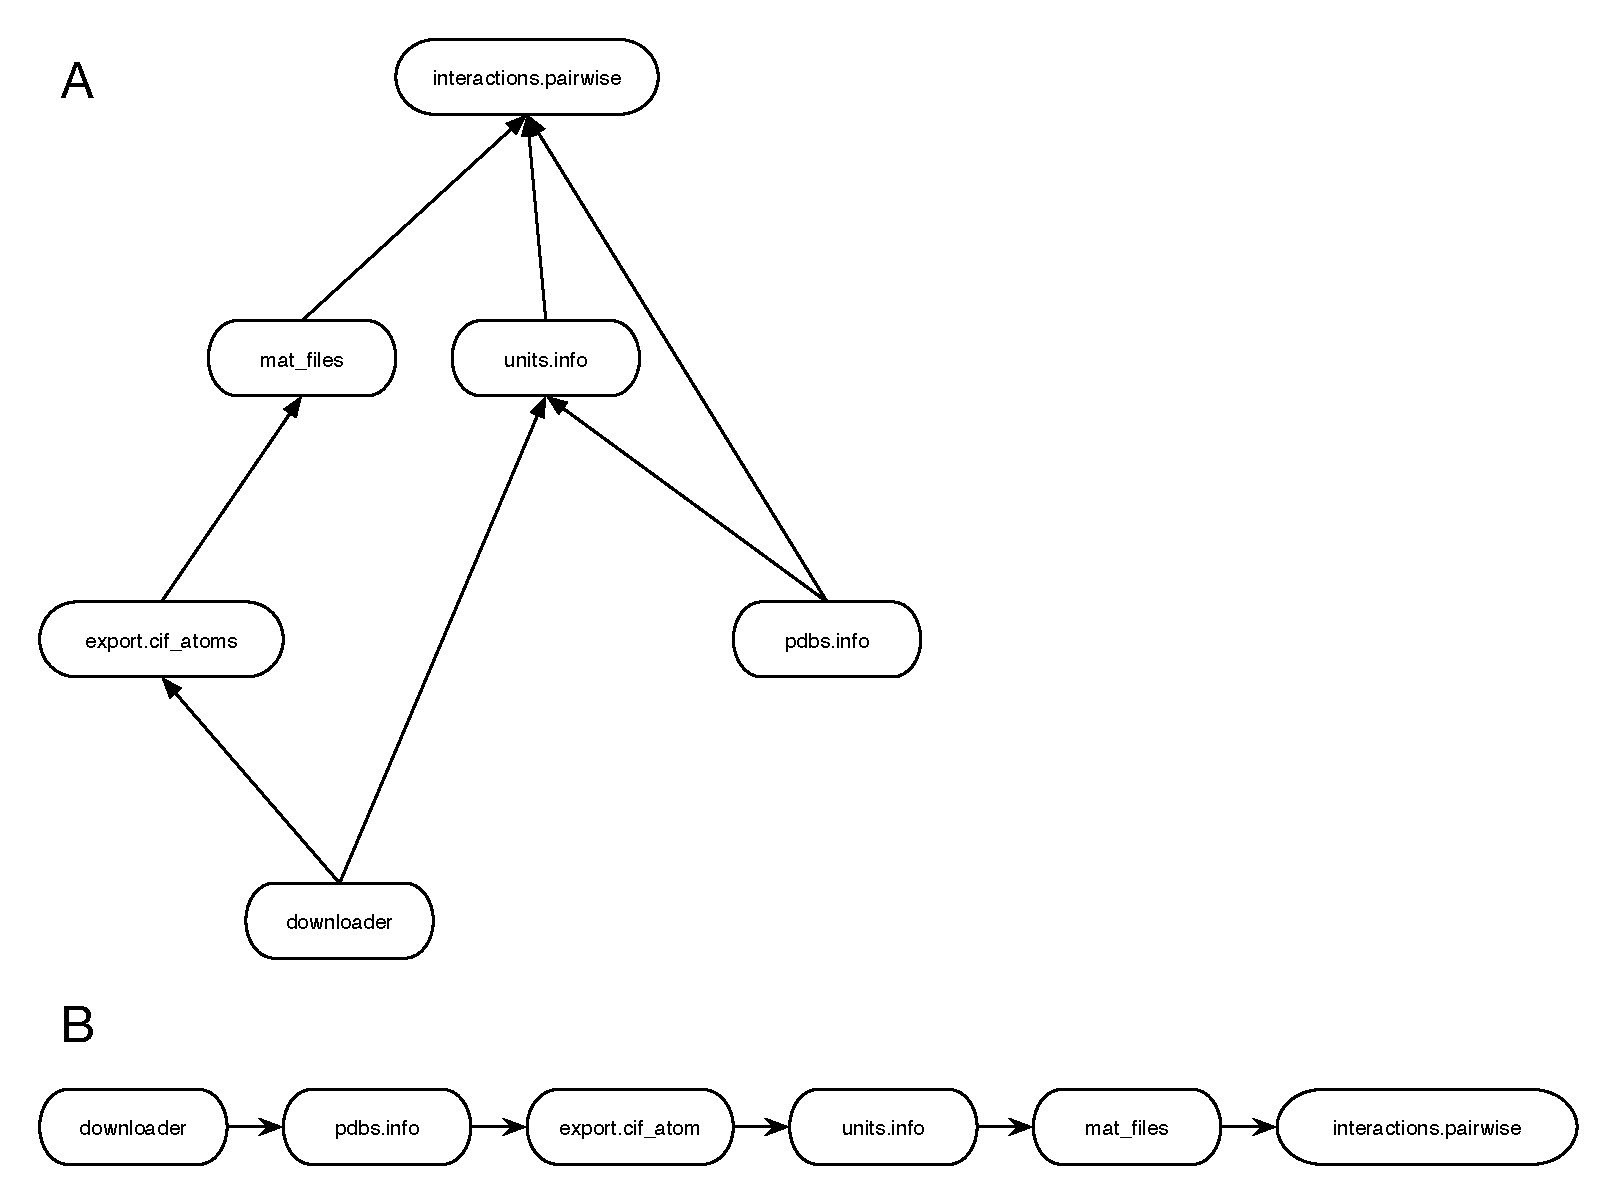
\includegraphics[width=\linewidth]{chapter-2/figs/deps}
  \caption{An example of an unsorted dependency graph (top) and a topological
    sorted dependency graph (bottom). Each stage is represented by an oval with
    the name of the stage in the oval. In this case the user has requested that
    the ``interactions.pairwise'' stage is run. This stage depends on two other
    stages, ``mat\_files'' and ``units.info'' as shown by the connections to those
    stages. Those stages have further dependencies. Shown in the bottom is the
    result of topological sorting the stages.}
\label{fig:stage-deps}
\end{figure}

With dependencies encoded in the pipeline, operators of the pipeline can request
the pipeline run a set of stages at once. In addition, part of the input to the
pipeline may optionally specify which dependencies do not need to be run. This
allows for the expression of complex requirements like, ``rerun all unit level
annotations except the distance and coordinate computation'. This is often
useful when testing out new parts or after fixing failed runs. When running all
structures, simply checking which input needs to be processed can take several
hours for some stages. When fixing a failed run or testing a new annotation, the
programmer will often already know which stages have been run. By instructing
the pipeline to run only those stages that are needed the overall run time can
be decreased.

With the previous version, to accomplish something similar to this it was
necessary to edit the code each time. I did this on several occasions and found
that it was very possible to forget that some parts were edited, since
computations could take hours, and in doing so left the code in a bad state for
the next weekly update. Because some parts were edited we did not run a complete
pipeline, leading to unexpected failures. This was then fixed by undoing the
edits that I previously made. Providing the capability to the pipeline operator
to what to run we avoid this problem entirely.

In addition, the main entry point now accepts either a list of PDB structures to
process or options to fetch the structures to run. The options and their usage
is explained in more detail in the ``Operation of the pipeline'' section. The
previous version always used all structures by default. While this is typically
the case, there are many situations where the operator wants to alter the
operation of the pipeline. For example, if one structure was not correctly
imported, only the failed structure should be rerun. By allowing the user to
select the structures specifically we make the pipeline easier to control.The
default mode of operation nonetheless remains. I have also added options to
allow selection of all structures that were available as of a specified date, or
prior to the current one. This has proven extremely useful when computing in old
releases during the update.

Operation of the the pipeline has been facilitated by implementing a single
entry point that takes as in input specifications for those parts parts to be
run and structures to be used. This ease of use also makes the pipeline more
reliable as it is no longer necessary to alter code to customize pipeline
operation.

\subsection{Making the pipeline robust to failures}

The pipeline will inevitably encounter errors during its operation. A robust
pipeline is one that gracefully fail. These errors can result from many sources.
The most obvious are mistakes in the code itself, for example, the pipeline may
have a bug in new code that causes it to attempts to for example, write invalid
quality data (a new feature). The second are errors introduced by external
resources. Part of our weekly update procedure is to fetch the list of all files
that are available as of the current date. This request to PDB can fail, because
all networks subject to intermittent failure. The final type of error is
mistakes in the input we are processing. For example, mmCIF files have certain
assumptions about their structure. In the past, some mmCIF files have not
respected their own assumptions leading to errors arising in the pipeline.I have
encountered all three types of errors and have worked to make the pipeline
robust in the face of these issues as discussed in the next paragraphs.

For the first set of errors, bugs in the code itself, I have added extensive
error handling code. The handling covers all aspects of the computing of and
saving of data to the database. Error handling identifies when errors occur and
alerts the user to the cause. Combined with extensive logging his aids in
debugging. The pipeline can cleanup, as required for validity, as well as
attempt to continue with other inputs. In addition, because the pipeline assumes
each input to a stage is independent and thus does not fail right away. This
leads the pipeline to attempting to compute data for all inputs to a stage prior
to failing. This provides a robustness against failures for specific inputs.

The next set of possible errors are those due to external resources. An example
of this type of work is fetching the quality report for a structure. PDB
provides quality data for all structures on their FTP site, which the pipeline
fetches for import. These requests can fail because of an unstable network.
However, these network errors are transient. The best way to handle network
errors is by identifying them as such and resubmitting the request.

I have modified the pipeline to retry requests to all external resources. Since
any request may fail due to network errors, the pipeline is now programmed to
always retry when a network error is encountered. It will retry up to the
specified number of attempts before failing. This allows for the pipeline to
deal with intermittent network failures, but not persistent failures. Longer
term issues such as a complete failure of the network will still cause the
pipeline to fail. However, this is acceptable since the pipeline could not
compute the required data. In addition, the requests can validate their
response. This helps with dealing in errors that happen when external sites
claim they sent data but the pipeline receives no data. For example, in the past
when querying PDB's services to attain the list of all files, PDB's response was
empty. This is not true as at the time about 2000 files were available, however
due to some error in their services we received a response stating there files
available.

The final type of issue, mistakes in the input data, does not have a simple
solution. Throughout the code, I have added checks to ensure the data is valid.
This allows confidence that the data being computed is correct. However, there
is no general purpose reusable way to always check that the mmCIF file is
formatted correctly. In addition we cannot simply retry computations as the data
will still be formatted incorrectly leading to the same errors. I dealt with the
issue mentioned above, a mmCIF violating its own design assumptions with
additions to the mmCIF reader to deal with this specific issue. I have added
extensive logging to the pipeline so that when this type of issues arises again
it will be flagged.

\subsection{Ease of extension}

The pipeline must be easy to extend. In order to make this possible I have
centralized all the essential logic of the pipeline into a few core classes that
can be inherited when creating a new stage. A class according to wikipedia is
"an extensible program-code-template for creating objects, providing initial
values for state (member variables) and implementations of behavior (member
functions or methods" (CITE
https://en.wikipedia.org/wiki/Class\_(computer\_programming)). Python, which the
pipeline is mostly written in, is an object-oriented language and users
interested in working with it are strongly recommended to study the language.
The majority of the pipeline is written using an intermediate or beginner level
of python. None of the advanced features, metaclasses for example, are used. I
will attempt to explain some fundamentals of python and object-oriented
programming here.

Classes can ``inherit'' behaviors from other classes. This is commonly done
through ``inheritance'. Inheritance is a common feature of object oriented
programming where in there is a base class or parent which defines some
functionality. From there one or more classes ``inherit'' the functionality and
are called ``child'' classes. This relationship forms a hierarchy of classes. The
behavior of any class is defined by the code in the class and all parent
classes. The child class can then extend the parent class functionality by
adding new behaviors. In addition, the child may override the parent class
behaviors by providing it's own implementation of specific behaviors. The child
implementation of any behavior is always prefered over the parent behavior.

In the pipeline there is a parent class that defines the overall stage flow
shown in Figure~\ref{fig:stage-flow}. Users can add a  new stages, called the
``child'' class, which ``inherit'' from this parent class and receives all the
standard behaviors such as deleting failed imports and only recomputing when
needed. A user may decide that some stage should never delete data in the case
of a failed import. For example, our loop ids are meant to never change and
allowing automatic deletion may cause issues. Thus if we want to be safe the
class that implements the logic of importing loops overrides the deleting
behavior to do nothing except log an error.

Because classes inherit the essential functionality of the pipeline, new users will only have to
implement 1) the logic for querying the database to see if this structure has already been
processed and 2) the logic to create the data to store.
Operation of the pipeline
In this section, I discuss the RNA.BGSU.EDU pipeline at a high level, to familiarize readers with
its functionality, organization, operation and documentation. Salient details will be provided,and
complete references will be provided to direct readers to the relevant sections of the detailed
documentation. We begin with an overview of the structure of the code and of the application,
followed by configuration options, and end with directions for running the pipeline.

\section{Execution of the pipeline}

The pipeline is a Python and matlab application that is publically accessible at
\href{https://github.com/BGSU-RNA/RNA-3D-Hub-core}. Detailed documentation is
available for the python code at \href{http://rna-3d-hub-core.readthedocs.io/}.
Our relational database is MySQL and the schema is not currently public.

The application is organized into a series of directories, as shown in
Figure~\ref{fig:pipeline-organization}. This figure displays the key directories
and explains their contents.

\begin{figure}
  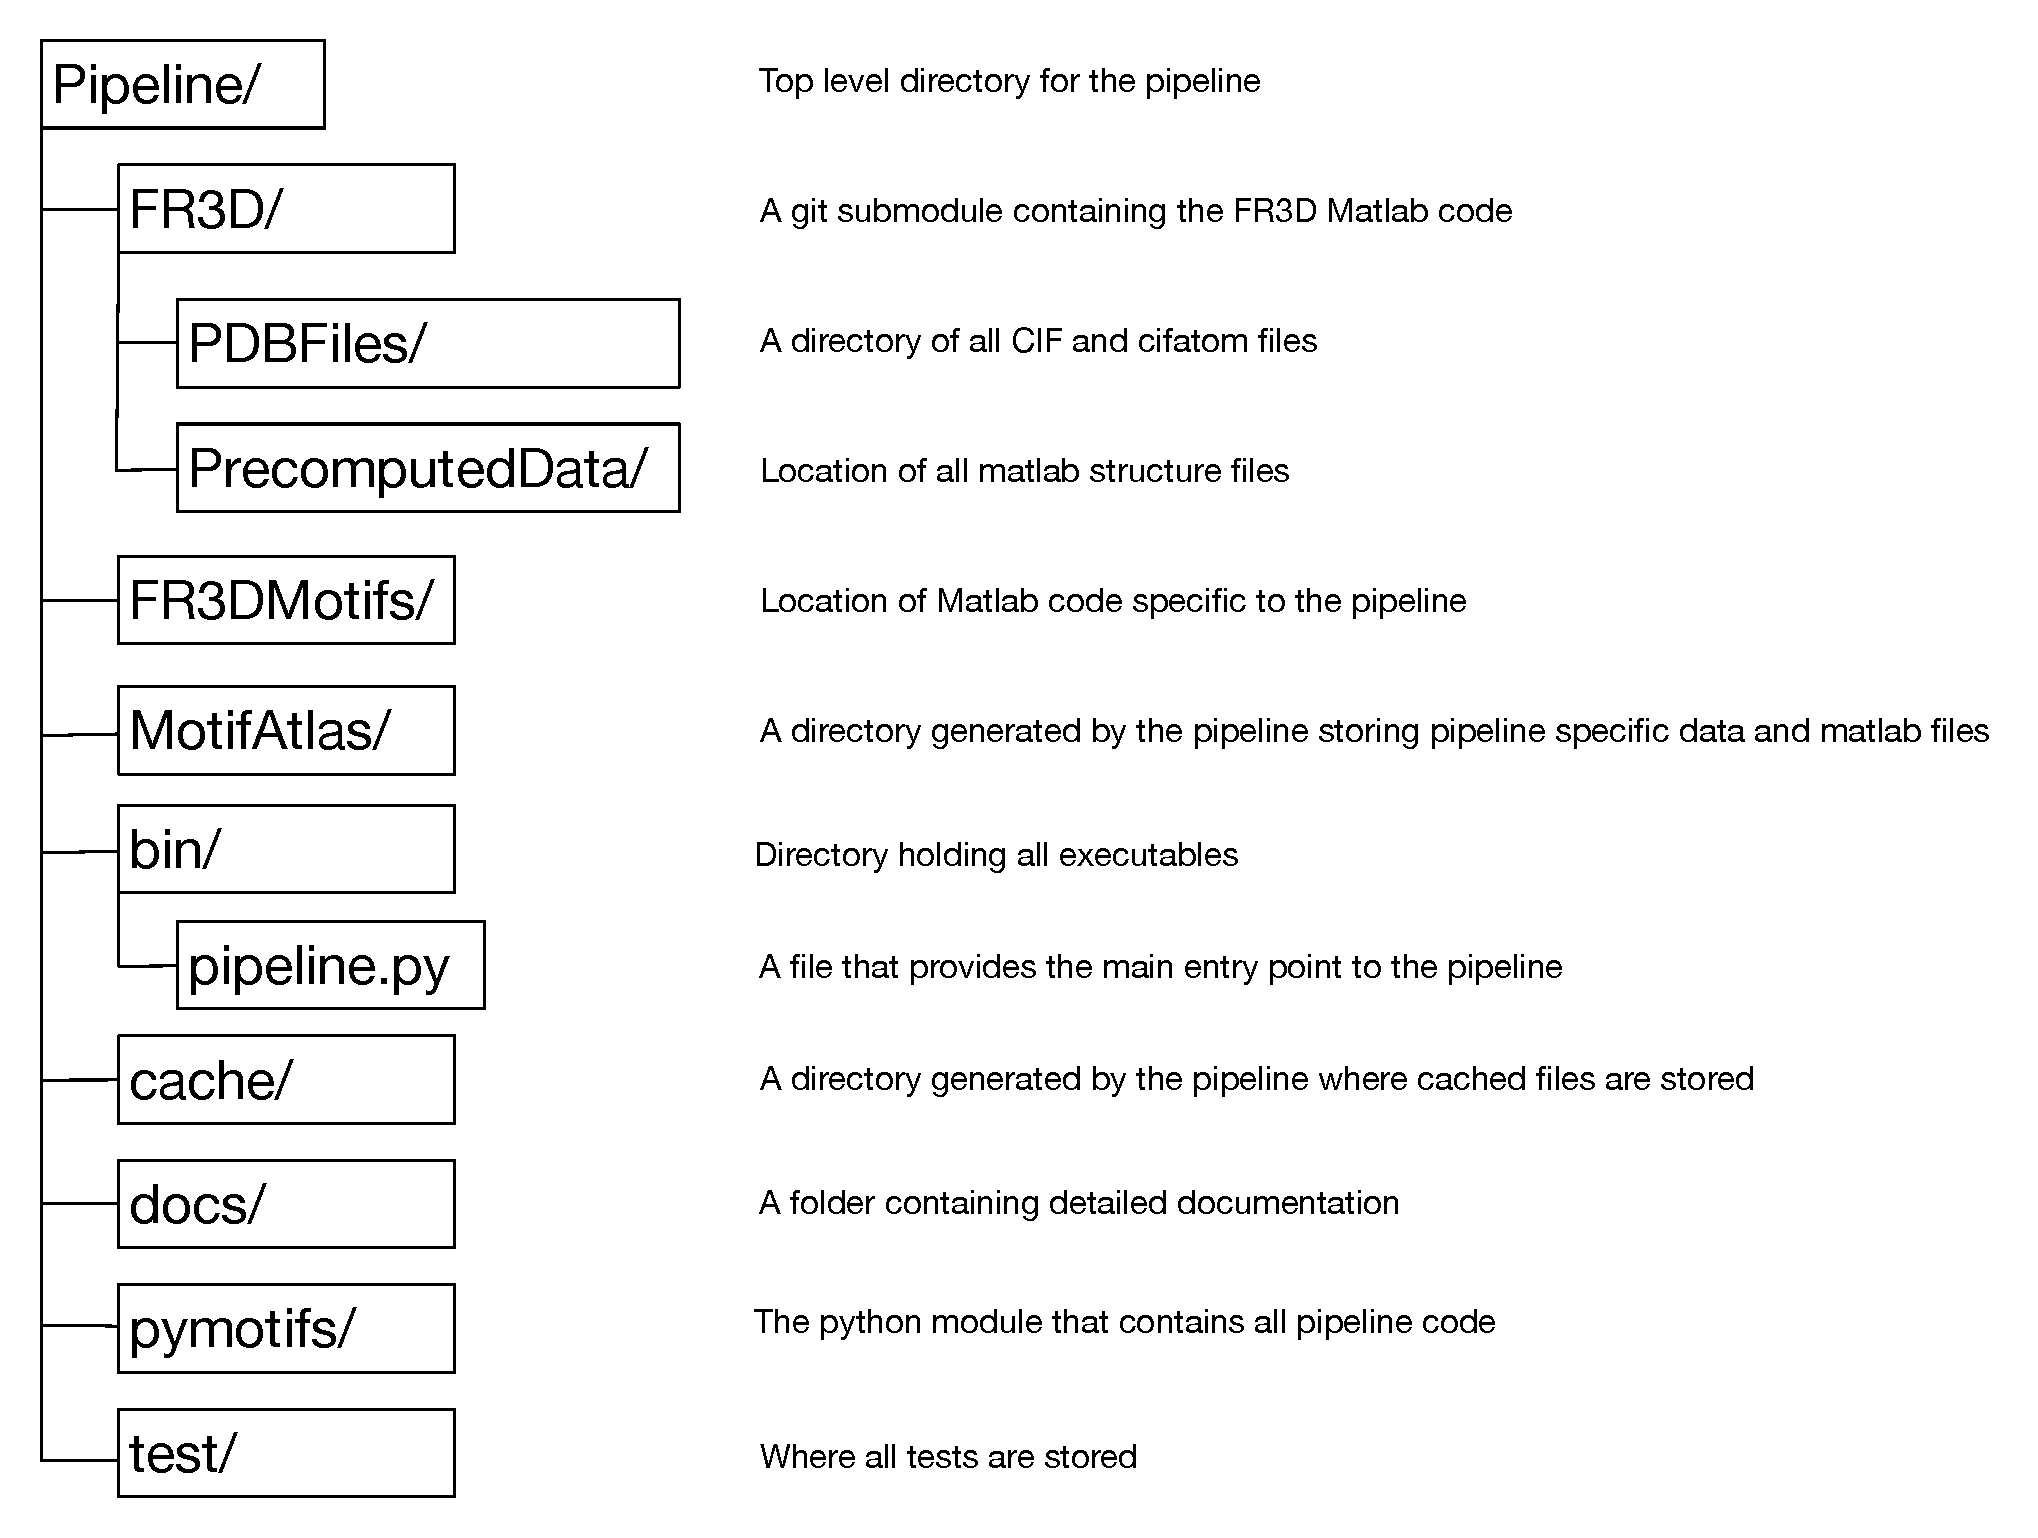
\includegraphics[width=\linewidth]{chapter-2/figs/directories}
\caption{Directory structure of the RNA BGSU pipeline. This figure shows the top
level and important directories in the pipeline. The directories are indicated
by ending with a ``/', while files do not end with a ``/'.}
\label{fig:pipeline-organization}
\end{figure}

\subsection{Configuring the pipeline}

Several important values, such as the database to use are configured in an
external file. The pipeline is configured through a JSON file that defaults to
``conf/motifatlas.json'. There are many possible configuration values, as
discussed in the detailed documentation. Table~\ref{tab:pipeline-config}
contains the key options. An example configuration file is included at
``conf/motifatlas.json.txt'' that can be modified to a simple working file. The
most important configuration value is the ``db.uri'' value which configures the
SQLAlchemy URI for the database connection. This specifies the database which to
connect to as well as the username and password. The user must be able to modify
the database, as well as add, delete and modify rows.

In addition, there are three file and directory paths which must be specified.
The first is the path to the matlab script that can execute matlab on the
command line. On linux systems this can be found using ``which matlab'' at the
command line and defaults to ``/usr/local/bin/matlab'. On OSX this will be in the
``bin/matlab'' directory below the matlab application. This means the default
location is ``/Applications/MATLAB\_R2013a.app/bin/matlab', for Matlab 2013a. The
second is where to write the loop export files. Part of the pipeline is an
export of all loops along with motif assignments. The file to write to must be
specified. Finally, the path to write interaction exports to must be specified
as well. Both the loop export an interaction export must be in a writeable
directory for the use the pipeline runs as.

Finally, the release\_mode section configures how the version numbers for motif
atlas, non- redundant and loops will be bumped. All releases follow the same
naming scheme of ``major.minor'. For example the NR release ``2.0'' has major
version ``2'' and minor ``0'. The minor can increments as much as needed and does
not influence the major version. When the major increments the minor is reset to
0. When the release\_mode is set to ``minor'' this will increment the minor part
of the version number, while ``major'' will cause the major to be bumped.
Generally, the release\_mode should be set to ``minor'. The only time ``major'
should be used is when there are large changes to the algorithm used for the
underlying algorithm.

\begin{table}[ht]
\begin{tabulary}{\linewidth}{LR}
\toprule
Variable & Purpose \\
\midrule

db.uri & SQLAlchemly uri string to specify the database to connect to \\

release\_mode.loops & A string, either ``major'' or ``minor'' to indicate
                        incrementing the major or minor version for loop releases \\

release\_mode.motifs & A string, either ``major'' or ``minor'' to indicate bumping
                        the major or minor version for motif releases \\

release\_mode.nr & A string, either ``major'' or ``minor'' to indicate bumping the
                   major or minor version for non- redundant releases \\

locations.mlab\_app & Path to matlab executable. \\

locations.interactions\_gz & Path to where the interactions export file is
                   written. \\

locations.loops\_gz & Path to where the loops export is written. \\

\bottomrule
\end{tabulary}
\caption{Main configuration options for the pipeline. All options show here must
  be provided.}
\label{tab:pipeline-config}
\end{table}

\subsection{Executing the pipeline}

The main entry point of the pipeline is the ``bin/pipeline.py'' python script. For
this discussion the script will be written as ``pipeline.py'. This script uses a
common ``subcommand'' ``options'' ``arguments'' design that will be familiar to anyone
who has used command line tools such as git. The top level command has a
``--help'' option which provides help information about the entire pipeline. In
addition, each subcommand also has a ``--help'' option to provide help information
about that command. Users should use this functionality extensively when
becoming familiar with the pipeline. In general a command to run the pipeline
looks like:

\begin{alltt}
pipeline.py [options] <subcommand> [options] [arguments]
\end{alltt}

Where $<>$ indicates a required value and $[]$ indicates an optional
value.

The pipeline provides several sets of functional facilities as shown in
Table~\ref{tab:pipeline-functionality}. This table shows each subcommand along
with the functionality it provides.

\begin{table}[ht]
\begin{tabular}{lr}
\toprule
Name & Functionality \\
\midrule
about & Get information about a stage \\
bootstrap & Populate the testing database \\
correct & A group of commands for correcting issues in the database \\
list & List the known stages and provide a breif overview \\
report & Create reports for external analysis \\
run & Run stage(s) \\
ss & Commands for importing 2D diagrams \\
transfer & Export/Import data from versions of this database \\
\bottomrule
\end{tabular}
\caption{Listing of all functionalities in the pipeline}
\label{tab:pipeline-functionality}
\end{table}

For the purposes of this section I will only discuss the import/export
functionality in the ``run'' subcommand. The main inputs to this command are the
stage to run and the structures to run it on. It takes a variety of options as
well. These options control the behavior of the pipeline. A summary of the
command is shown in Figure~\ref{fig:running-options}. Here we will discuss how
the options and arguments connect to our overall goals as well as how to achieve
some specific tasks.


\begin{figure}
\begin{alltt}
Usage: pipeline.py run [OPTIONS] NAME [IDS]...

  Run specific stages of the pipeline.

  'run' accepts as input the stage to run and a list of PDB ids to import
  and process. It determines the order of dependences and executes them in
  the correct order.

Options:
  --dry-run            Alter nothing while running
  --skip-dependencies  Skip stage(s)
  --skip-stage TEXT    Stage to skip
  --seed INTEGER       Set the random seed
  --recalculate STAGE  Recalculate data for the given stage(s)
  --all                Use all RNA containing PDBS
  --known              Use only downloaded files
  --after-date DATE    Get files posted after DATE (YYYY-MM-DD)
  --before-date DATE   Get files posted before DATE (YYYY-MM-DD)
  --exclude PDB        Excluded PDB(s)
  --ignore-time        Ignore time for rerunning
  -h, --help           Show this message and exit.
\end{alltt}
\caption{A summary of the options and arguments for the ``run'' subcommand.}
\label{fig:running-options}
\end{figure}

An important goal of our design has been to provide the user to ability to
choose the structures to process as well as the annotation data to compute. The
first was achieved by providing PDB ids as input. This input can be provided
manually when needed. It will process the files given and the user can input
them manually. As it is often the case that all available files, or all files
available by a date are wanted the pipeline accepts options which will determine
what files match that criteria. In addition, it is possible to then exclude
structures from that list using the given files.

The second goal, control over which data are computed, is done by putting the
stage to run as input to the pipeline. This provides the user precise control
over what is run. By default the pipeline will run all dependencies of the stage
as well the stage itself. This ensures that the required data are available for
the requested stage. When the user is sure that no dependencies need to be run,
I have added options to skip all dependencies ({\tt --skip-dependencies} ) or skip
specific stages ({\tt --skip-stage stage}).

Another goal is to avoid recomputing data already computed.where it is necessary
to over this default setting, the {\tt --recalculate stage} option can be used.
This option will force the pipeline to recompute all data for the given stage.
The {\tt .} stage name refers to the stage given so: {\tt pipeline.py run
--recalculate ``.'' --all units.info} will force a recompute for the units.info
stage, but not it's dependencies. To force all stages that are run to recompute,
the user can use the {\tt *} argument. For example {\tt pipeline.py run --all
--recalculate ``*'' units.info} will recompute all stages that are run for all
structures.

Examples that show how to use the described options and arguments will clarify
the usage. Below we list a series of tasks and the corresponding command
(displayed as {\tt monospaced font}).

\begin{description}
        \item [Run an update on all structures]
                {\tt pipeline.py run --all update}

        \item [Import pairwise interactions for 1FJG]
                {\tt pipeline.py run interactions.pairwise 1FJG}

        \item [Import all unit annotations for all structures]
                {\tt pipeline.py run --all units.loader}

        \item [Import all unit annotations for all structures skipping structure 2AW7]
                {\tt pipeline.py run --all --skip-pdb 2AW7 units.loader}

        \item [Create an NR group for 1FJG, 1J5E, 1S72]
                {\tt pipeline.py run nr.loader 1FJG 1J5E 1S72}

        \item [Compute all interaction annotations for all structures while skipping all dependencies]
                {\tt pipeline.py run --skip-dependencies --all interactions.loader}

        \item [Import loops in all structures]
                {\tt pipeline.py run --skip-stage loops.quality --all loops.loader}

                This command runs all loop level annotations, while skipping the loop quality stage,
                which is generally only needed before doing a motif atlas import, and simply is not
                needed importing loops, thus the reason it is skipped.

        \item [Recalculate all pairwise interactions]
                {\tt pipeline.py run --recalculate . --recalculate mat\_files interactions.pairwise}

                Note that for this command we have to recalculate all
                {\tt mat\_file}'' as well as the interaction import. This is
                because the {\tt mat\_files} stage controls the creation of the
                precomputed data that the matlab programs use. If we do not
                specify recomputing the mat files the process will simply
                reimport the already existing annotations.


        \item [Build a motif atlas using structures in the ``structures'' file]
                {\tt cat structures | xargs pipeline.py run motifs.loader}

                The structures file should contain only the ids to use, with one
                per line. The ``xargs'' command is required because the pipeline
                does not read from standard input and so xargs transforms the
                call to include the ids as part of the call. Note that there is
                a system dependent limit for the number of arguments allowed to
                a command. The limit is generally in the thousands.
\end{description}

\subsection{Testing the pipeline}

The pipeline is tested through two related methods. First, there is a script
that will run the pipeline on 70 structures to populate a test database. The
process of creating a database to work with is called ``bootstrapping''. The
structures to use are stored in ``pymotifs.constants.BOOTSTRAPPING'' and have been
chosen because they have caused crashes or errors in the past. In the future as
more problematic structures are found they should be added to the set of
structures used in testing.

The bootstrap script can be run using the command {\tt bin/pipeline.py bootstrap}.
Bootstrapping requires a special configuration file in conf/bootstrap.json. It
does not use the standard configuration file because it is important to have a
separate testing and development database. Otherwise it is possible to
accidentally overwrite or modify data that is required for tests. This can lead
to spurious test failures and waste developer time. Bootstrapping will run the
pipeline several times because one of the major parts of the pipeline is
computation of changes of groupings over time. By running it more than once on
different sets of structures we can test this important functionality.

The bootstrapping serves two purposes. The first is to populate a database the
test scripts can work with. The second is to provide a high level test of the
pipeline. By running the full pipeline on many structures we are increase the
chance of detecting blatant errors in the code. For example, bugs that prevent
the pipeline from being run will be caught here. Issues where a foreign key
constraint violation may appear here as well. This serves as a good initial
method to test the overall functionality of the pipeline and is recommended
before deploying a new stage.

The second way the pipeline is tested by ``unit testing'' components of the
pipeline. We test individual methods of classes using the py.test library. This
is a very traditional method of testing python applications. The tests are
stored in test/ and are organized into a hierarchy that parallels that of the
main program, making it simple to determine which module is being tested for
each test file. Test file names must end with ``\_test.py''. For example, the
tests for the units.info stage are in ``test/units/info\_test.py''.  There is very
extensive documentation on writing tests and readers are strongly encouraged to
read documentation on writing unit tests in python and using py.test. Examples
of such links are: 
\begin{itemize}
  \item \url{https://stackoverflow.com/questions/3371255/writing-unit-tests-in-python-how-do-i-start}
  \item \url{http://docs.pytest.org/en/latest/}
  \item \url{https://jeffknupp.com/blog/2013/12/09/improve-your-python-understanding-unit-testing/}
  \item \url{https://docs.python.org/2/library/unittest.html}.
\end{itemize}

Here we give a quick overview of testing in python, as well as information on
the parts that are unique to this pipeline.

In python, tests are often organized into classes. We use this approach
extensively in the tests. It is important to know that it is not needed, as
py.test will use simple functions as tests as well. Readers interested in that
approach should read py.test's documentation on this. We use classes because of
the organization advantages it provides. For test classes, if there is a ``setUp''
method that takes no arguments it is run prior to any tests. This method is used
to setup any data or objects that are needed for testing. As discussed below
this is used to setup stages for testing correctly. Each test method must start
with the string ``test\_'. Within them there should be an assertion about the
computed and expected value. Ideally tests are as simple as possible and contain
only 1 statement to compute the value to test, 1 statement to define the answer
and 1 statement to assert the computed value equals the expected value. This is
standard unit testing in python. The reader is encouraged to read more extensive
documentation and advice on this subject.

The test classes that test a stage in the pipeline must inherit from the
StageTest class from the test module. These classes should also have a
``loader\_class'' attribute which specifies the class of the stage to test. This
stage will be initialized in the StageTest's ``setUp'' method. The object will be
built using the configuration specified in ``conf/bootstrap.json''. As with
standard python tests this method is run prior to all test methods. Classes
which implement their own setUp method must have a call to the superclass's
setUp method. Without this the stage will not be initialized correctly.

Another useful functionality of the test suite is the ``skip\_without\_matlab''
annotation. This is to be used on any test that calls matlab. It allows the test
suite to run without crashing on machines that do not have matlab, or the python
to matlab connector, installed.

One useful extension to the testing methodology currently used is to automate
testing using a service like \href{https://travis-ci.org/}{Travis CI}. This
service reruns all tests whenever someone pushes code to the github repository.
Such testing has been implemented for the fr3d-python repository and can be seen
at \url{http://www.travis-ci.org/BGSU-RNA/fr3d-python}. Travis CI and related tools
are now standard in software development. This approach has not been used with
the pipeline for two reasons. First, setting up the database is a long and
complex procedure. The bootstrap script takes nearly half a day to run and
produces several gigabytes of data. Secondly, Travis CI and all services like it
do not have matlab installed as this is a commercial product. While the
skip\_without\_matlab annotation will ensure that other tests do not fail, it will
mean that key functionality that matlab provides will not be tested. This may
result in tests passing even though they are actually failing in an environment
with matlab. Thus we should not use the service as long as we continue to rely
on Matlab code.

It should be possible to deal with these issues by first, removing matlab from
the pipeline. Once all of FR3D's functionality is written in python the pipeline
will be testable with standard tools. Secondly, something will have to be done
to either decrease the number structures tested or make it quicker to load the
results of bootstrapping to the database. It may be possible to use a database
dump to rebuild the testing database, but that will pose problems with keeping
it up-to-date, but is worth exploring. Using a dump would mean the testing on
travis would not require the bootstrapping process, allowing for tests to be
completed quickly. Future developers should look into using tools like Travis CI
to improve the testing and reliability of the pipeline.

\chapter{GROUPING RNA 3D STRUCTURES FROM FROM PDB USING MMCIF FILES IN RNA INTO
EQUIVALENCE SETS}

\section{Introduction}

This chapter reports changes implemented to improve modules of the data pipeline
that calculates Equivalence Classes of RNA entities of RNA 3D structures for the
Nucleic Acids Database (NDB) and for RNA.BGSU.EDU. The 3D structures are
provided by the Protein DataBank (PDB).

The PDB is an archival resource that serves as  the accumulated scientific
investigation of the 3D structures of macromolecular entities of biological
significance. The earliest entries date back to the late 1960s and early 1970s
and new entries are accumulating at an ever-increasing rate. The earliest RNA
entries were structures of dinucleotides and the latest entries include entire
ribosome structures bound to a variety of tRNA and mRNA substrates and
translation factors. But structures containing smaller RNA molecules bound to
enzymes that modify them or use them as guide RNAs  to recognize other
substrates continue to accumulate. Thus there is a huge variation in the size of
the RNA entities and of the scientific purposes for which the investigation was
conducted.

\section{Previous work}

We have previously implemented a method to group RNA molecules into equivalence
sets. The method is described in Nonredundant 3D Structure Datasets for RNA
Knowledge Extraction and Benchmarking \cite{Leontis2012b}. The current work is
an extension of these methods so, we begin by briefly describing the previous
methodology which was developed when 3D structures were still distributed in PDB
files, so that like large structures like 70S ribosomes had to be split over two
or more files. At that time it was convenient to simply select the largest chain
in a file and use to represent the RNA in the file for grouping. In cases where
the file also had one or more smaller chains the smaller ones were ignored and
no groups built for them. For example, structures of a large ribosomal subunit
contain both the 23S and 5S in the same file, the 5S was simply ignored and not
extracted and clustered separately. Each chain was compared on the basis of
sequence alignment, species and geometric discrepancy to all other chains. The
previous method did not compute all possible sequence alignments or
discrepancies due to runtime issues. The alignments and discrepancies were not
stored for future studies.

\section{Motivation for current work}

We have one main motivation for updating our RNA chain grouping method. The
first is to take advantage of technical changes data and secondly are to enhance
the scientific utility of our resources by providing a more complete set of data
that includes all chains found in RNA structures.

Recently,  PDB has migrated from “PDB” formatted structure files to the new
macromolecular Chemical Information File format (mmCIF), which made it possible
to store structural information for macromolecular complexes of any size in just
one computer file. By contrast, the out-dated PDB format was limited to no more
than 99,999 numbered atom data records per file. This change has made possible
the storage of all ribosomal subunits, large subunit, small subunit, tRNA, mRNA
fragments, 5S and 5.8S (for eukaryotes) into a single file. In some files such
as 4V4Q \cite{Schuwirth2005} more than one entire ribosome is present. Because
our old method only considered the largest chain in each file we would ignore
all chains except a single LSU. This would lead to ignoring many important
groups.

There are a number of scientific use cases for which our RNA structure classes
and derived data will be  3D structures in the PDB/NDB and these are worth
enumerating and discussing.

\begin{enumerate}
  \item Determining the breadth and depth of solved structures, ie the number of
    distinct types of RNA and the number of each type.

  \item Statistical studies of recurrent elements of RNA structure, RNA-RNA and
    RNA-protein interactions

  \item Comparative studies of similar or homologous RNA structures and
    RNA-protein complexes

  \item Functional studies of RNA structural flexibility, variation and
    conformational change in response to environmental perturbations

  \item Comparative assessment of RNA structure modeling quality and reliability

  \item Compilation of modular RNA parts for synthetic biology and RNA
    nanotechnology

  \item Analysis of  of RNA sequence variation to improve RNA structure
    prediction and understanding of RNA evolution
\end{enumerate}

Thus, the change to mmCIF format required a complete rethinking of the
procedures for extracting, naming, and clustering RNA entities and has enabled
significant improvements in the results. This chapter describes those changes
and the choices made to maximize the value of the data for diverse scientific
users.

\section{Types of molecules and requirements}

In this section we will highlight specific groups that pose special challenges
for clustering to motivate the following sections were the methods developed are
explained and their success in correctly clustering these special cases is
assessed.

\subsection{Ribosomal RNA subunits}

The largest entities are ribosomal RNAs (rRNA), which comprises the large (LSU)
and small (SSU) ribosomal subunits, the 5S rRNA, and the 5.8S rRNA in
eukaryotes. LSU and SSU from a number of species representing all three major
phylogenetic domains and mitochondria are presently available.

The rRNAs should be divided into separate Equivalence Classes (EC) as follows:
First, each of the SSU rRNAs (mitochondrial 12S, bacterial 16S and eukaryal 18S
rRNAs) should be placed into their own EC by organism. Each of the 23S rRNAs
from archaeal or eubacterial ribosomes should be placed in distinct EC. The 5S
rRNAs, which are found in the LSU of all ribosomes except some mitochondrial
ones, should also be in a separate group. While bacterial 5S rRNA does interact
directly with 23S rRNA in the LSU, it does so through non-Watson-Crick pairing
and backbone interactions involving its loop E internal loop (IL) motif and a
similar structured IL of helix 38 of 23S rRNA. The loop E of 5S rRNA has been
shown to assume the same 3D conformation in the absence of 23S rRNA and so is
not dependent on 23S to form its native state. The same holds for eukaryal 5S
rRNAs, each of which are placed in their own EC.

By contrast 5.8S rRNA of eukaryal LSU, constitutes an integral part of the large
ribosomal RNAs (26S or 28S, depending on the species), as they are homologous to
the 5’-ends of bacterial 23S rRNAs. As such they form extensive Watson-Crick
interactions with the larger rRNA of the LSU in which they occur and so,
according to the criteria defined above, belong together in the same RNA entity
, for the purposes of grouping.

In addition, the ribosome has long been an molecule of study. Early structures
\cite{Mueller2000} often were resolved at very low resolution. These structures,
while informative, are not as useful for current work as more recent high
resolution structures. While we want to group all structures it is very useful
to create groups of structures with similar resolution. In the past we have
found using resolution cutoffs of 1.5{\AA}, 2.0{\AA}, 2.5{\AA}, 3.0{\AA}, 3.5{\AA}, 4.0{\AA}, 20.0{\AA}, and
‘all’ a group of all structures regardless of resolution create useful groups.
Here we continue this practice.

From these examples we can see that the members of groups should be one or more
chains which interact extensively through watson crick base pairing should be
placed as a single entity and then grouped with other such entities. We can see
that the groups should only contain molecules from the same species. In the case
of large molecules this can be determined through sequence alignments alone.
In addition, all members of a group should fall within a resolution cutoff.

\subsection{tRNA and mRNA complexes}

tRNA molecules are commonly solved in the context of their binding to a
ribosome. In these cases they are often also bound to an mRNA fragment. These
mRNA fragments can span the A and P sites of the rRNA and have two tRNA’s bound.
The mRNA fragments (6 bases) are very small and are extensively bound to the
tRNA as all bases are paired with the tRNA. Despite this we do not want to place
the tRNA’s and mRNA into a single entity for grouping. In this case we believe
the most scientifically meaningful unit is the tRNA. The small mRNA fragment is
not interesting alone. It is small and contains no internal structure. Thus
while we do want to place two chains which extensively pair into a single unit
we do not want small unstructured chains connecting two larger structured
chains. For the purposes of grouping all chains we will allow the small
unstructured chain to ‘accompany’ the larger chains. But it should not be used
to connect the two structured chains.

The tRNA case also provides another case to consider. It is well known that some
initiator tRNA's from different species have the same sequence. This implies we
cannot use sequence alignments alone to separate molecules from different
organisms. However, there authors provide a source organism annotation.
Investigations into this annotation have showed that while many are precise some
annotations include the terms ‘synthetic compound’ or are not provided. These
chains often have identical sequence to another annotate chain. In other cases
the synthetic chain aligns very well to a correctly annotated chain. Thus we can
treat synthetic or no annotation as being similar to any other annotated
species.

These issues, the fact that some molecules from different organisms will have
identical sequences, and the potential issues with author annotations shows us
that while we should use alignments and organism assignments to connect members
of a group we must provide another criteria. We must enforce that each group
contain a single species, ignoring the assignments to synthetic. This will
maintain our requirement that groups contain only members from the same species.

\subsection{Small model compounds}

A great deal of detailed structural information has been provided by studies of
small model compounds. These compounds are often two strands which bind to form
a small helix with loops. For example studies of the isolated sarcin-ricin motif
(CITE: 4NLF) have provided detailed information on its structure. In these
structures the unit we should cluster is the duplex. Like the LSU and 5.8S each
strand interact extensively through Watson-Crick base pairs. However, these
strands have no internal structure. There are also model compounds, such as the
nano square that are composed of 8 chains \cite{Dibrov2011a}.

From these examples we can see that we should be able to join any number of
unstructured chains together to form a single unit for grouping. This is
different from the case of multiple tRNA's on a small mRNA fragment where the
two tRNA's would not form a single unit. Here we want the chains, even if they
are not directly interacting, to form a single unit.

Many of these small model compounds differ from one another from due to single
nucleotide changes. These changes are intentional and so we require that small
molecules have identical sequences in our grouping.

\subsection{Small Protein and RNA complexes}

Several proteins have been solved with small bound RNA's. These RNAs are often
poly-A or other such simple sequences. These chains may agree in sequence and
species assignments but they differ in assigned geometry due to binding by the
protein. These chains should be split even if they are similar on the basis of
sequence and species. Thus our groupings should be sensitive to the overall
geometry of the members.

\section{Criteria for equivalence classes and their members}

These examples show first of all, that many CIF miles contain more than one
chain. Second the example of Eukaryotic LSU rRNA show that the members of some
EC may be one or more chains in contrast to our previous EC. A prerequisite of
grouping is to define the RNA-containing entities to be extracted from structure
files as precisely as possible and in a manner that is biologically relevant for
the purposes of most users of the resource. Guided by giving priority to
biological relevance, we settled on the following definition of the relevant
RNA-containing entities: The entities to be identified and extracted from
PDB/NDB structure files are “groups of one or more RNA chains that form
identifiable integrated structural and functional units.” Internally we refer to
these entities as “RNA integrated functional elements” or “RNA IFEs.” We will
use the term “IFE” as a short-hand for this definition.  Most RNA IFEs consist
of a single chain, but some do not. The simplest examples comprise two chain
Watson-Crick paired chains forming a duplex structure: strictly, this comprises
two molecules, but effectively it is a single entity or RNA IFE.

From these examples we can see there are 3 requirements for each EC.
\begin{enumerate}
  \item Two IFE’s included in the same Equivalence Class should come from the
    same biological source. The intention of this criterion is to separate
    homologous RNA molecules, for example SSU rRNAs from different organisms,
    into distinct Equivalence Classes.

  \item Two IFE’s included in the same IFE should have very similar, though not
    necessarily identical sequences. This criterion may seem redundant with the
    first criterion. The intention is to include sequence variants (for example
    16S rRNAs coded by different genes of the same micro-organism that differ in
    a small number of positions) but to separate molecules with similar
    sequences from evolutionarily related organisms that belong to distinct
    species. We note that not all RNA chains in PDB are labeled with a
    biological source, which complicates clustering.

  \item Two IFE’s included in the same Equivalence Class should have the similar
    conformations and geometries. The intention of this criterion is to separate
    instances in which there is a significant conformational change, even when
    the RNA sequence(s)and biological source  are the same. For example, poly-A
    bound to poly-A binding protein (PAB) (PDB 1CVJ) has a different
    conformation from poly A forming a parallel strand duplex (PDB 4JRD). These
    IFE’s are structurally dissimilar and should not be in the same equivalence
    set, even though the sequence may be identical.

  \item Two IFE’s included in the same EC should have similar resolution.
\end{enumerate}

However, we decided to group structures together even though their sizes differ
when:

\begin{enumerate}
  \item The same molecule was used in the experiment as reported in the CIF data
    field ``poly\_seq\_scheme''. In some cases only part of the molecule was
    resolved. Because the experiment was using the same molecule we believe it
    should be grouped with the other structures of the same, but larger
    molecule.

  \item The observed part superposes well with the corresponding parts of more
    completely resolved structures.

  \item The observed structure is a small part of the overall molecule. For
    example, there are structures of a single domain of the ribosome
    \cite{Nissen2000}. These structures are best grouped with the other
    ribosomal structures as that is the context they are just a small portion of
    the larger complex.
\end{enumerate}

In addition, there are several other cases where we assign IFE’s to the same
equivalence set:

\begin{enumerate}
  \item We group IFE’s together EVEN WHEN their geometries differ significantly
    when the structures are too low resolution as the data are not adequate to
    quantify the structural differences.

  \item Structures belong together even when RNA is bound to different proteins
    or ligands but they have when they have very similar geometries. At present,
    it is not our intention to classify PDB structures at the level of
    RNA-protein complexes. For this study we focus on the RNA components of the
    structure.
\end{enumerate}

There are several important implications of these requirements. First it is
possible that the homologous RNA molecules (for example iso-accepting tRNAs)
from different species have nearly identical sequences and structures.
Nonetheless they will be placed in different groups In addition, it is possible
that two groups will have similar sequence and species but differ only in
geometry.

\section{Methodology for building Equivalence Sets}

In this section we discuss the process of building equivalence sets. The overall
process is to
\begin{enumerate}
  \item Identify and extract RNA chains

  \item Build RNA IFE's from individual chains.

  \item Link pairs of IFE's by sequence similarity, source species, and
    geometric similarity.

  \item Extend equivalence sets using transitivity of similarity links

  \item Assign names

  \item Display data on our Website

  \item Share data with NDB
\end{enumerate}
Below we discuss each step in detail and how it achieves our goals.

\subsection{Building RNA IFE's from individual chains}

We have implemented an algorithm for joining chains into IFE's. As discussed in
our examples the joining logic depends on whether or not a chain is
``structured''. Structured chains only get joined with other structured chains
they directly interact with, and they must make a significant number of
interactions with them. Unstructured chains are always joined any chain they
interact with, but they will not indirectly join two structured chains together.

Our algorithm operates as follows. We first mark all chains in a structure as
``structured'' or ``unstructured''. A ``structured' chain is defined by having at
least 5 internal (within the same chain) cis Watson Crick/Watson Crick (cWW)
basepairs. We then join chains based upon a few rules. A representation of these
rules is shown in Figure~\ref{fig:build-ife}.

\begin{figure}
  \includegraphics[width=\linewidth]{chapter-3/figs/build-ifes}
  \caption{The rules for building connecting chains into IFE's. Each chain is
    represented by a circle. Unstructured chains are in blue with the letter
    ``U'', while structured chains are orange in ``S''. The left side indicates the
    input and the right shows the possible results of each case. On the left the
    dotted lines indicate one or more cWW interactions between the chains. On
    the right each grey circle indicate an IFE built of the two chains. For case
    1 and 2 we always join the two chains into one IFE, while in case 3 it
    depends upon the number of interactions. Case 4 shows that for two
    structured chains selected by an unstructured chain the two structured
    chains are placed in separate IFE’s while the unstructured chain is placed
  in both IFE's.}
  \label{fig:build-ife}
\end{figure}

In this figure we can see the four basic cases. First when determining if we
unstructured chains should be connected, we always connect them if they have any
cWW interactions between them. This allows for joining of separate stands of
duplexes. In the second case we always connect unstructured chains to structured
chains. This serves to connect unstructured fragments such as mRNA’s to the
structure tRNA’s they are interacting with. For connecting two structured chains
we require that the maximal ratio of external cWW to internal basepairs is at
least 0.6. This is an experimental determined cutoff. It may be adjusted in the
future. To examine if this cutoff is reasonable we produced the figures shown in
Figure~\ref{fig:ext-vs-int}.

\begin{figure}
  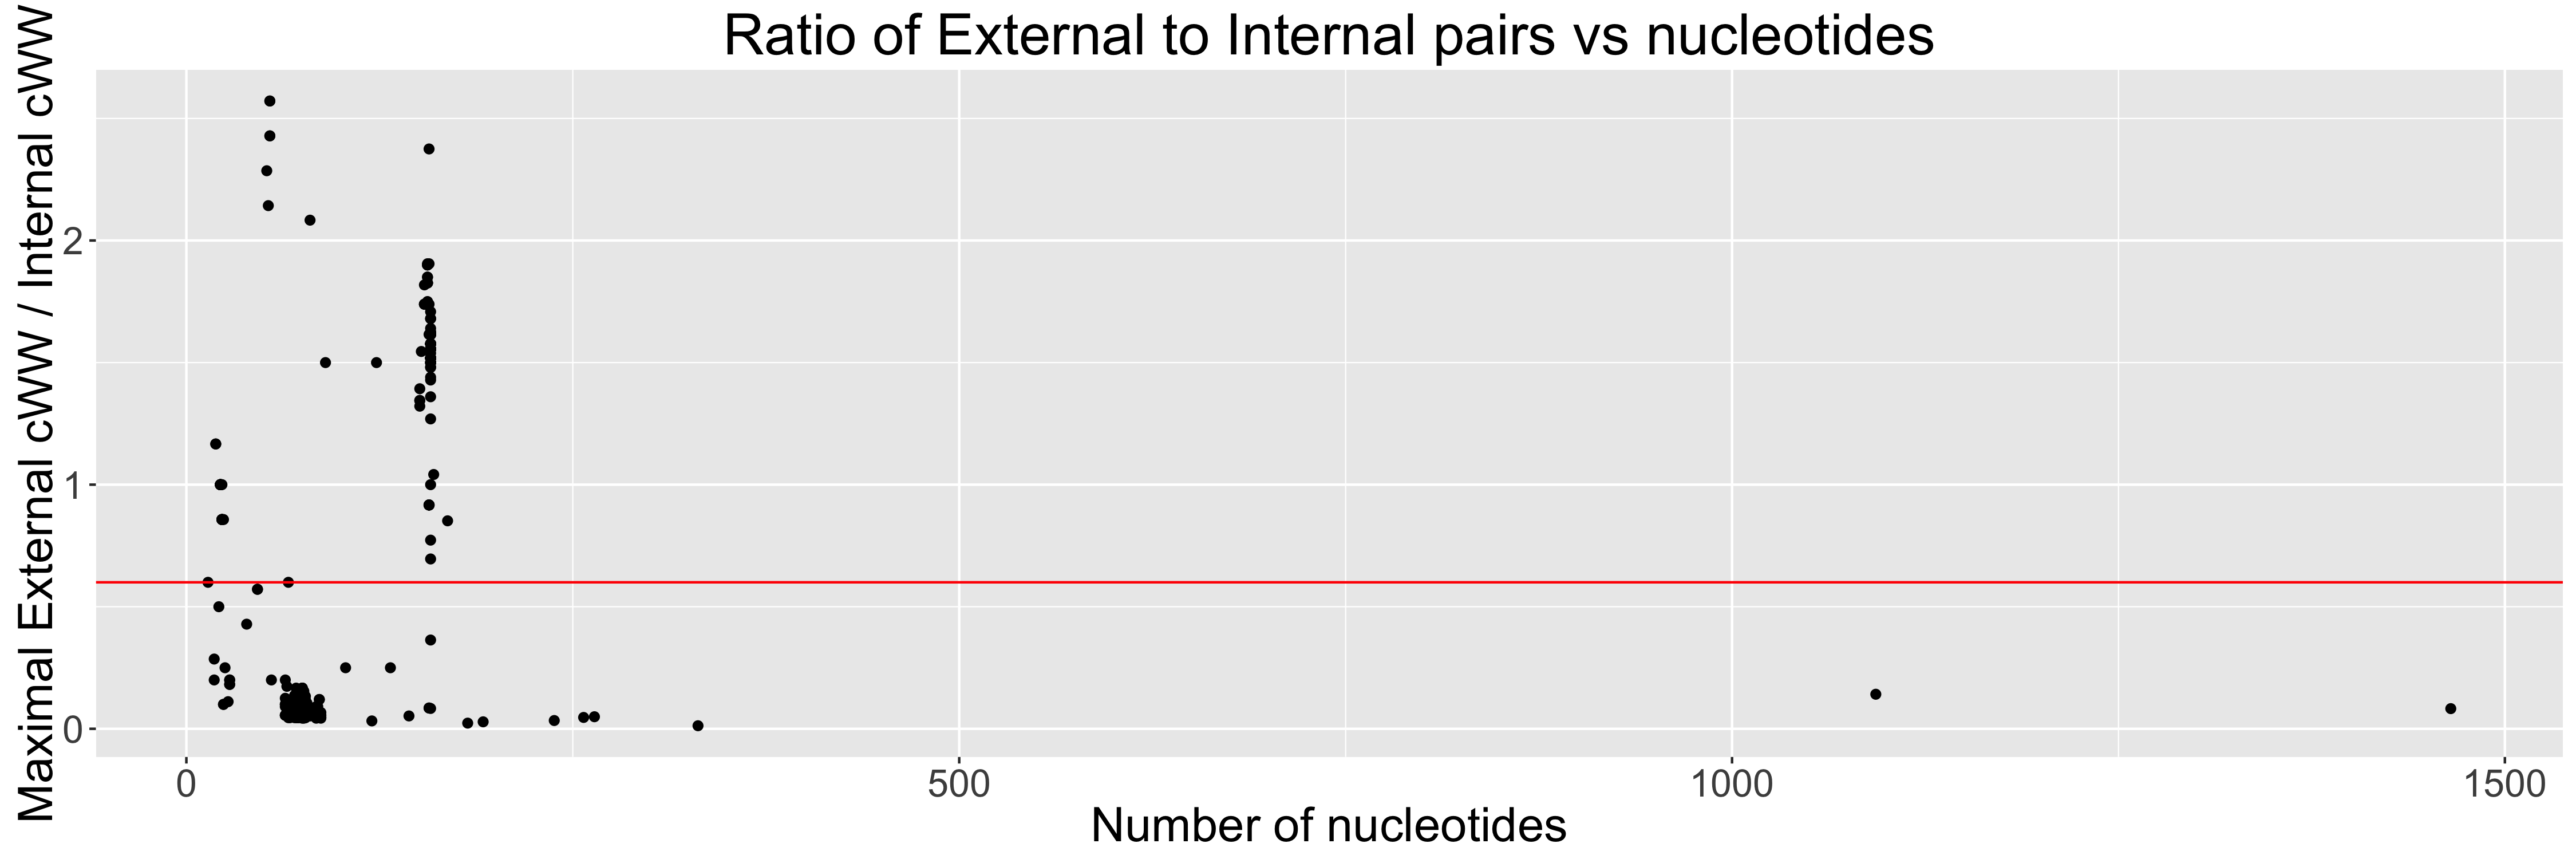
\includegraphics[width=\linewidth]{chapter-3/figs/internal-external}
  \caption{Summary of the ratio of external to internal base pairs. The leftmost
    panel shows a histogram of the maximal ratio of external to internal pairs
  for all pairs of chains which have an interaction between them. }
  \label{fig:ext-vs-int}
\end{figure}

\subsection{Connecting pairs of IFE's to from equivalence sets}

To build equivalence sets we compare all pairs of IFE’s based upon their species
assignments, their alignment, their discrepancy. Pairs of chains which have a
valid alignment, are from similar species and have a discrepancy of less than
0.4{\AA}, if computed, are joined. We then build the EQ sets by placing all chains
which are transitively connected into one set.

The steps are:
\begin{enumerate}
  \item Determine the species assignment for all chains.
  \item Compute the alignment of all pairs of alignable chains.
  \item Compute the discrepancy between all chains which have a good alignment
\end{enumerate}

The first step requires looking up the assigned phylogeny for chain. Many chains
are assigned to a particular species making the lookup trivial, however some are
assigned to a subspecies. For these cases we use the parent species of the
chain. However, not all chains are assigned to an organism, many are marked as
‘synthetic construct’ or not assigned any organism. In both of these cases we
treat the organism as synthetic. In addition, a few chains (3) are assigned to a
genus rather than a species or sub-species, in these cases we treat the chain as
being synthetic as well.

In order to compute the alignments between all pairs of chains correctly and in
a reasonable time frame we align experimental sequences. Experimental sequences
are the sequences used in the experiment and may differ from what is observed in
the experiment. Often the solved structure will have ‘gaps’ indicating where
bases were not resolved. For example EXAMPLE. In order to build alignments
correctly we use the experimental sequence. If we did not we would have to
ensure that the resulting alignments respected gaps in the both chains. The
alignments would  have to have breaks where the observed chains have breaks.
This is a difficult problem and it is simpler to use the experimental sequences
where this is not a concern.

In addition, by using experimental sequences we reduce the number of required
alignments. It is very common to use the same molecule in many experiments. For
example, there are many structures of the same E. coli ribosome with different
tRNA’s or antibiotics. All of these structures can be represented by a few
experimental sequences. There is no need to realign sequences simply because
they came from different experiments, the alignments will be the same.

We also require that all the pairs of experimental sequences to align  have
similar size. The rules for size depend upon the size of the chain. The specific
rules are shown in TABLE SIZE RULES. The reason for the size constraint is to
reduce the number of required alignments while ensuring that we perform all
required alignments. For our purposes an alignment between a large and small
subunit will never provide any information so we avoid computing them.

Finally, we require that the experimental sequences have either been assigned to
the same species or one of them has been assigned to synthetic. We refer to this
as the chains having a similar species. This ensures that we are only comparing
sequences which could be from the same source. We have observed that some
experimental sequences are assigned ‘synthetic’ in one experiment are assigned a
species such as E. coli in another experiment. Thus we allow the comparison of
synthetic chains to any other chain, so long as it has similar size. The last
step is to compute the discrepancy. Discrepancy is a measure of geometric
similarity like RMSD but it is sensitive to the base orientation and position.
It has been used extensively in our lab for searching RNA 3D Structures
\cite{Sarver2008a}, building NR sets in the past \cite{Leontis2012b}, as well as
building motif groups \cite{Petrov2013}. We only use the first structured chain
in each IFE. While this is a simplification of the situation it has proven to
work well and makes the problem simpler. For discrepancy we are only interested
in chains that:

\begin{enumerate}
  \item Have a good alignment between them. As this discrepancy will be used to
    build EC, there is no need to compute it for chains that do not align well.
    These chains cannot be in the same EQ set so discrepancy is not needed. This
    reduces the number of comparisons needed making the computations much
    quicker.

  \item Have resolution less than 4.0{\AA} or are solved using NMR. We do not
    compute discrepancies for chains with poor resolution (greater than 4.0{\AA})
    because doing so provides artificially inflated value. Many structures of
    low resolution are helices which have not been modeled with planar paired
    bases. This modeling is inaccurate and produces high discrepancy when
    compared to carefully modeled helices. Because of this we split structures
    which should be joined. We however, do allow for comparisons using NMR
    because most NMR structures are very small and the errors introduced are
    small.

  \item Have at least 3 aligned bases. This is because discrepancy is only
    defined for at least 3 bases.

\end{enumerate}

With these rules we are able to efficiently compute all required discrepancies.
By doing this as part of our pipeline we are able to store these values. This
allows for comparison of grouping methodologies and constraints.

We then connect all pairs of IFE’s which satisfy the alignment, species and
discrepancy requirements. These connections are treated as a graph and used to
build equivalence classes through transitivity.

\subsection{Building equivalence classes from pairs of IFE’s}

We build EC through transitivity. This means that all connected IFE’s, even if
the connections are indirect, are placed into a single group. An example of such
a clustering is shown in Figure~\ref{fig:transitivity}.

\begin{figure}{ht}
  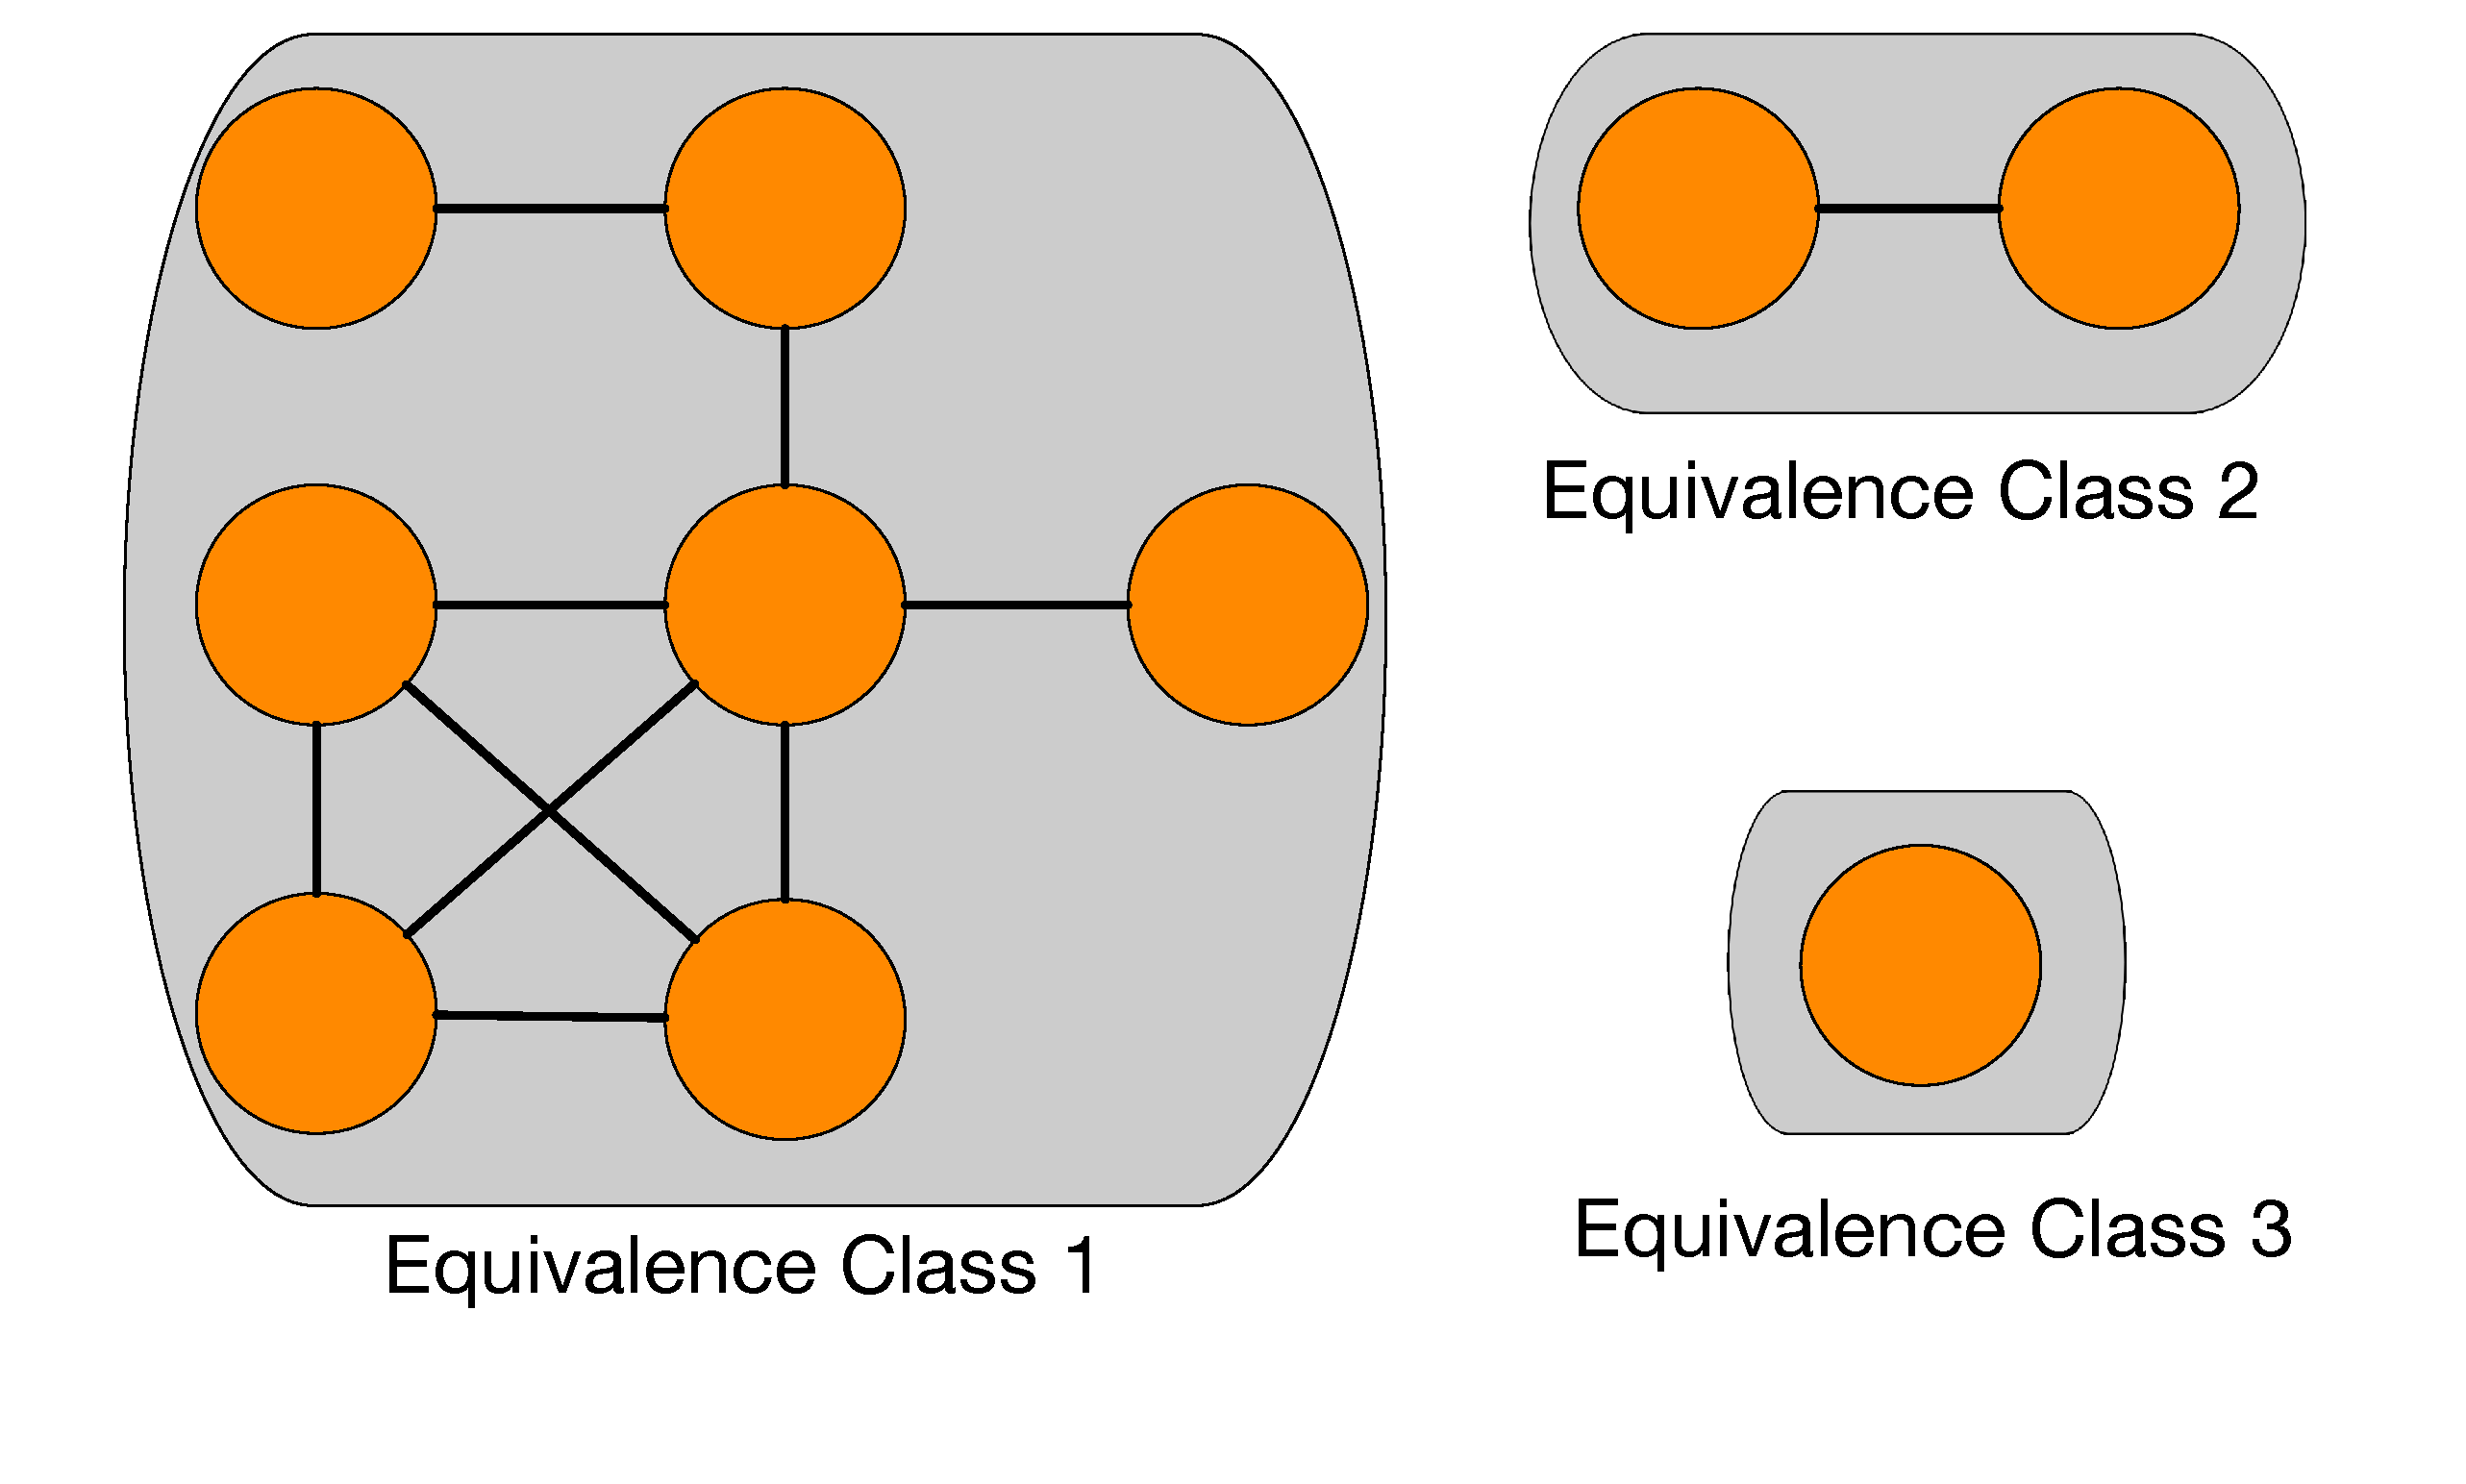
\includegraphics[width=\linewidth]{chapter-3/figs/ife-transtivity}
  \caption{Schema of Equivalence Classes built by transitivity. In this figure
    each IFE instance is represented by a circle.Lines connecting circles
    indicate pairs of IFE's having similar sequences, the same species and
    geometric discrepancy below the threshold value of 0.4. Each Equivalence
  Class is represented by the grey background around a set of circles. To in
included in a class an instance need only be connected to one other member of
the class.}
  \label{fig:transitivity}
\end{figure}

Using transitivity minimizes the number of singleton outlier groups. Most IFE’s
will compare well to at least one other, placing them in the same group. The use
case of studying structural variation in molecules. Without a transitive
grouping, structures which differ only in structure would be split from all
other instances. The groups are created using all possible structures, the ‘all’
resolution cutoff. From there the groups are filtered to only contain structures
which satisfy each resolution threshold. With the groups created, the only
remaining step is to name them

\subsection{Naming equivalence sets}

In previous work Dr. Anton Petrov created a naming scheme based upon the
parentage of the equivalence class \cite{Petrov2013}. I preserve the overall
scheme but have modified it in a significant way to make an easier to understand
system, as described next.

The naming scheme is as follows:
``NR\_{resolution\_cutoff}\_{unique\_handle}.{version}''. This scheme has 3
components, the resolution cutoff used, a unique randomly selected handle and
the version number for this group. The resolution cutoff provides information on
what the resolution is used to build the EQ set. The unique handle is a unique
randomly generated number that serves to make all ids unique.

We have changed the naming scheme so that the unique handle is identical across
all resolution cutoffs of the same set of structures. For example, an EQ set
built of tRNA’s at the ``all'' resolution cutoff may have the name:
``NR\_all\_00001.1''. At the 4.0{\AA} resolution cutoff this now would have the
name ``NR\_4.0\_00001.1''. This differs from the previous method where as
different randomly generated handle was assigned to each resolution cutoffs of
the same equivalence set. By making this change the random handle remains
identical across resolution cutoffs making it much easier to which EQ sets have
the same molecule.

\section{Results of Equivalence Set building}

For the purposes of this chapter we created an EQ grouping using all structures
available as of July 25, 2016. This grouping was then analyzed to see how the
resulting groups matched our objectives. I begin with a general description of
the clustering and then discuss each previously mentioned case in detail,
finally I examine the groupings of outliers.

\subsection{General properties}

I built a grouping using all PDB available from July 28, 2016. The grouping used
3213 PDB’s which contained 7015 IFE’s. These were grouped into 2168 EC’s. These
groups varied in size from 1 (singleton groups) to 377 instances. A summary of
the member count distribution is shown in in Table~\ref{tab:eq-size-dist}.

\begin{table}
  \begin{tabular}{lr}
    \toprule
    Number of instances & Number of Equivalence Classes (Percent of all classes) \\
    \midrule
    1               & 1352 (62.4\%) \\
    2-5             & 615 (28.3\%)  \\
    5-10            & 118 (5.4\%)   \\
    10-20           & 53 (2.4\%)    \\
    20-50           & 16 (0.7\%)    \\
    \textgreater 50 & 14 (0.6\%)    \\
    Total           & 2168 (100\%)  \\
    \bottomrule
  \end{tabular}
  \caption{Counts of the number of classes for a range of sizes. This table
    shows the number of classes for a range of sizes for the new grouping method
  for all 3213 structures available as of July 28, 2016}
  \label{tab:eq-size-dist}
\end{table}

The table shows a surprisingly high percentage, 62\%, of singleton groups. I
tested to see if this is consistent with the previous method by building a
grouping using the set of structures December 05, 2014 as shown in
Table~\ref{tab:compare-size-dist}. This date was chosen because it corresponds
to both the last grouping using our previous method as well as as the transition
to mmCIF data. These two datasets contain the same experimental results, however
there are fewer mmCIF files because many  of the PDB files have been merged into
a single mmCIF file. This gives us an ideal set to compare the two methods. From
the table we can see that the old and new method have similar performance, with
the new one having fewer singleton groups. Thus 62\% of our groups are singleton
groups for the July 28, 2016 data is not surprising when compared to the
previous groupings.

\begin{table}
  \begin{tabulary}{\linewidth}{LRR}
    \toprule
    Number of instances & 
    Number of Equivalence Classes in 2.0 & 
    Number of Equivalence Classes in 1.89 \\
    \midrule
    1               & 1081 (61.0\%)  & 1112 (78\%) \\
    2-5             & 527 (30.0\%)   & 234 (16\%)\\
    5-10            & 88 (5.0\%)     & 31 (2\%)  \\
    10-20           & 38 (2.0\%)     & 19 (1\%)  \\
    20-50           & 20 (1.0\%)     & 8 (0.5\%) \\
    \textgreater 50 & 11 (0.6\%)     & 5 (0.3\%) \\
    Total           & 1765 (100\%)   & 1409 (100\%) \\
    \bottomrule
  \end{tabulary}
  \caption{Comparison of new method to previous method. This table compares the
  performance of the previous and new method on the same data set of structures.
The data are taken from
\url{http://rna.bgsu.edu/rna3dhub/nrlist/download/2.0/all/csv}, which contains 2680
structures, and \url{http://rna.bgsu.edu/rna3dhub/nrlist/download/1.89/all/csv}
(contains 3145 structures) and represents all the structures available as of
December 5, 2014. The transition from 1.89 to 2.0 corresponds to the move from
PDB to mmCIF formats which decreased the total number of files, because many
previously separate files were merged}
  \label{tab:compare-size-dist}
\end{table}

I next moved to examine results of groups of particular interest. I begin with
the ribosomes, then tRNA’s, and then protein/RNA complexes.

\subsection{Ribosomal subunits}

As an example to evaluate the groupings of ribosomes, I examined the equivalence
classes containing the Thermus thermophilus small ribosomal subunit (SSU). We
constructed heatmaps of both the sequence similarity and the discrepancy between
all chains as shown in Figure~\ref{fig:tt-ssu-align} and
Figure~\ref{fig:tt-ssu-disc}. The alignment heatmap indicates the high sequence
similarity among all IFE’s. The geometric discrepancy heatmap shows that there
may be two main structurally groups in the equivalence class. Currently we are
exploring these groups to see if they correlate to biological states.

\begin{figure}[h]
  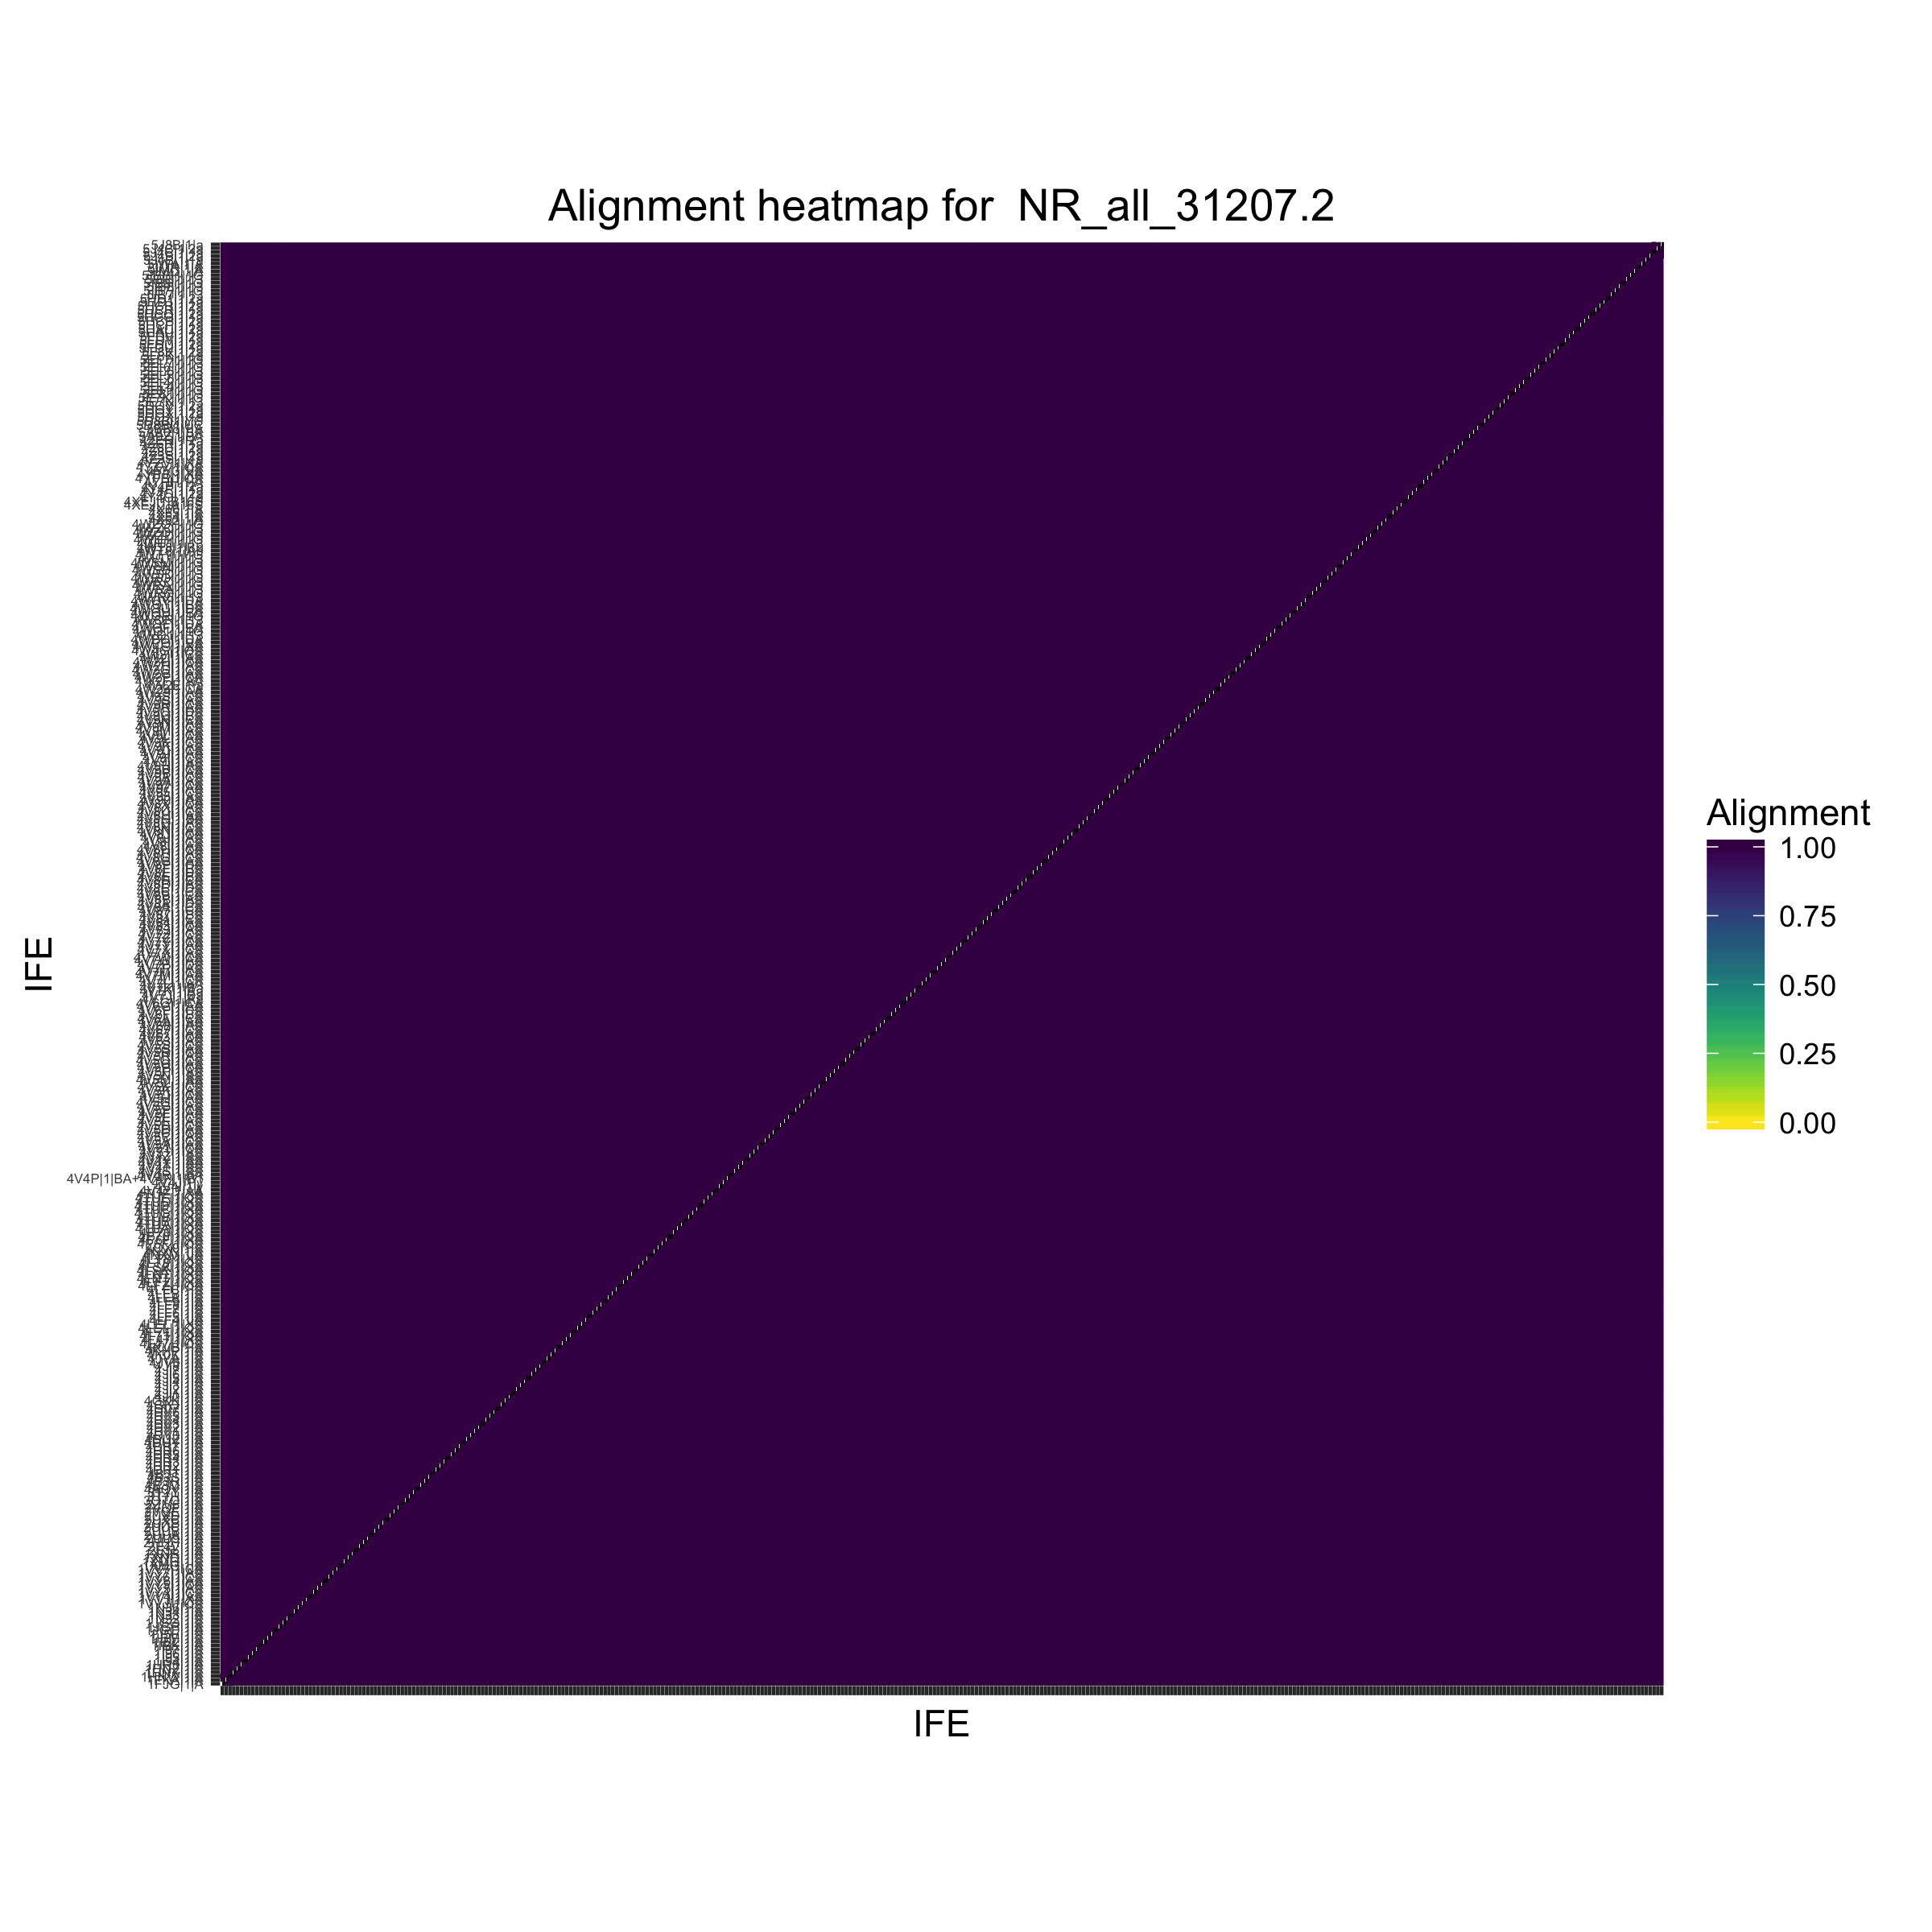
\includegraphics[width=\textwidth]{chapter-3/figs/tt-ssu-align}
  \caption{A figure summarizing the sequences similarity for all IFE’s in the
    Thermus thermophilus small subunit. Color scale indicates discrepancy
  values, lighter colors being worse.}
  \label{fig:tt-ssu-align}
\end{figure}

\begin{figure}[h]
  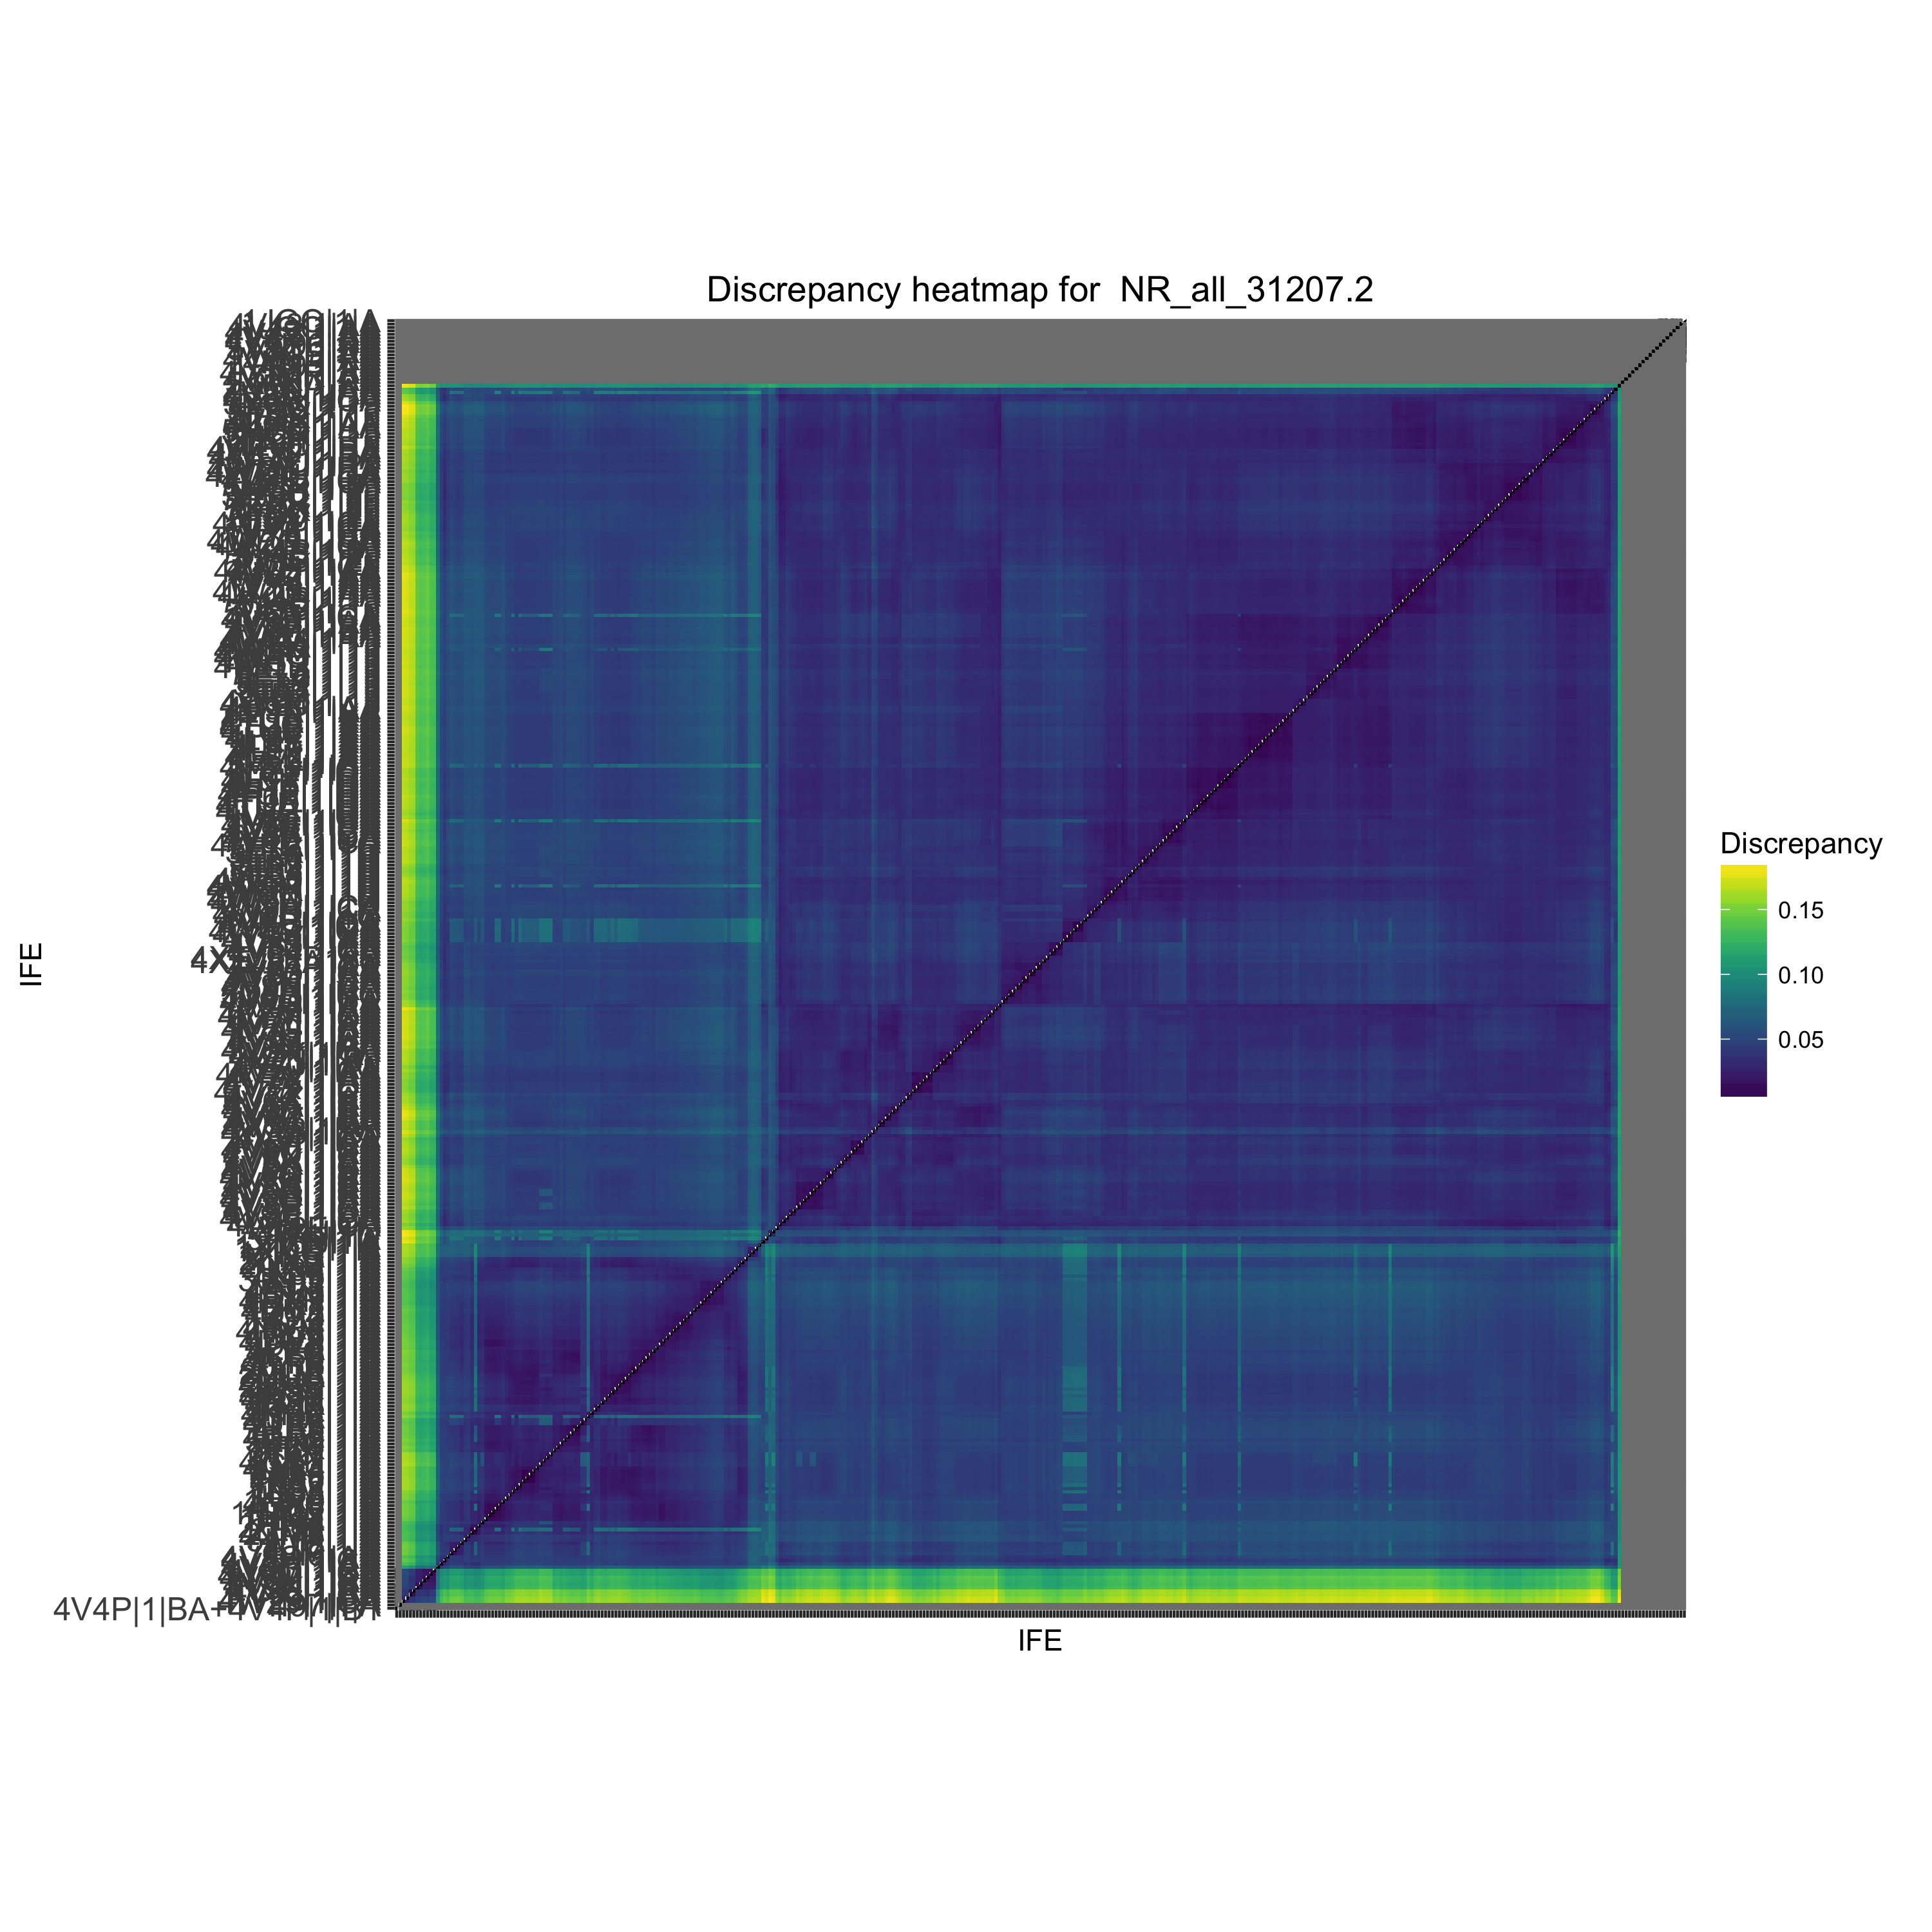
\includegraphics[width=\textwidth]{chapter-3/figs/tt-ssu-disc}
  \caption{Summary of the discrepancy for all pairs of IFE’s in the Thermus
    thermophilus small subunit. Grey squares indicate no data computed, because
    that structure has too low a resolution. Color scale indicates discrepancy
  values, lighter colors being worse.}
  \label{fig:tt-ssu-disc}
\end{figure}

\subsection{tRNA and mRNA complexes}

We examined two classes that contained tRNA alone and tRNA/mRNA complexes. The
tRNA only group is shown in Figure~\ref{fig:trna-alone}. In it we can see that all
chains are geometrically similar and have identical sequences. However, within
the group we can see that there are several subgroups, notably, 4WSM chains 2L
and 2K are geometrically distinct from all other members and similar to each
other. However, the differences are below our cutoff of 0.4 {\AA}/nt leading to them
being placed in the same group.

\begin{figure}[h]
  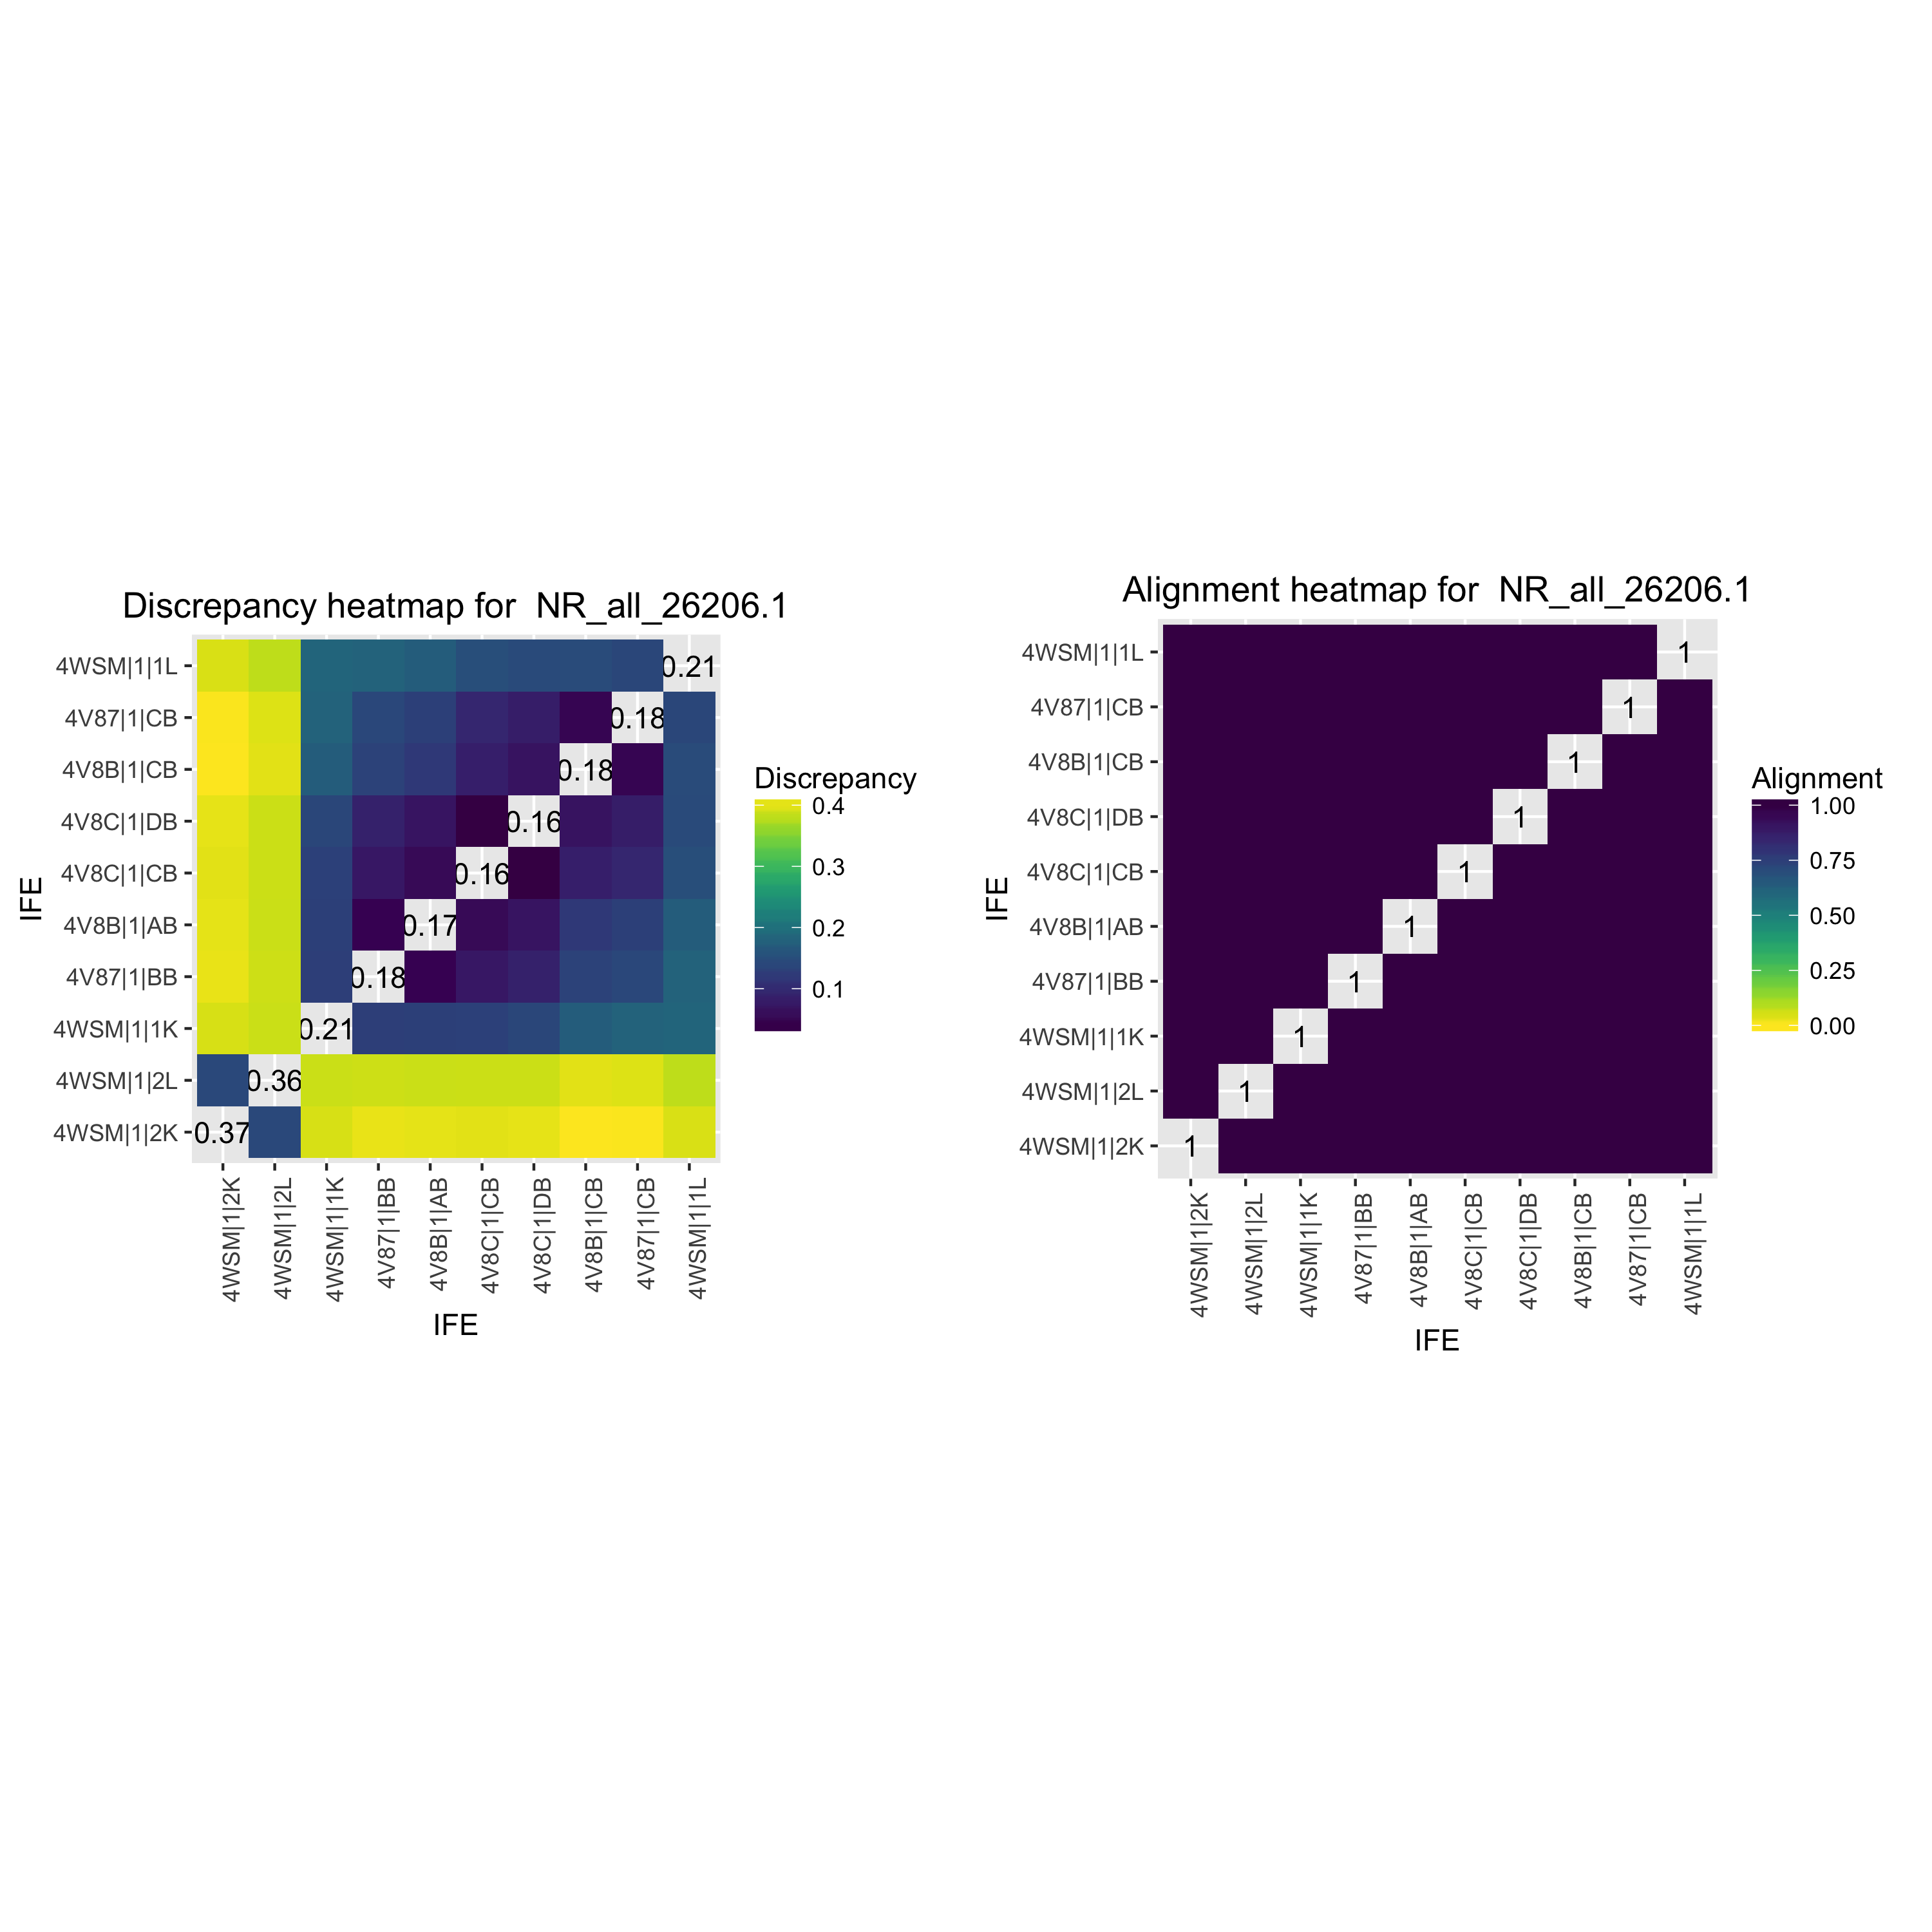
\includegraphics[width=\textwidth]{chapter-3/figs/trna-alone}
  \caption{Example of a tRNA/mRNA complex forming an equivalence class. On the
    left is a heat map of the discrepancies for all IFE’s in the group. The
    right shows the heat map of sequence similarity for the group. Color scales
    indicate the value, with lighter colors meaning ‘worse’ values. Along the
  diagonal of each plot is the mean value for each row.}
  \label{fig:trna-alone}
\end{figure}

\subsection{Protein and RNA complexes}

Small RNA/protein complexes are the groups which are most affected by usage of
discrepancy. To test how our method works we built a grouping with and without
discrepancy. We used a small, 11 nt, poly-A chain as a test case. This molecule
adopts different conformations depending upon the environment. In 4JRD it forms
a non-canonical duplex, while in 1CVJ it forms a single strand bound to a
protein. Shown in Figure~\ref{fig:small-aa-no-disc} we can see the discrepancy
of such a clustering. It contains several subgroups that are only connected
because we have not use discrepancy to split them. Upon using discrepancy this
group is partitioned into 4 other groups, one of which is shown in
Figure~\ref{fig:small-aa-disc}.  In this heatmap we can see that the group is
much more homogeneous and all pairs have discrepancy less than 0.2{\AA}/nt. In
addition all members of this group form a similar structure and are bound to
proteins, unlike the previous method where the group was a mix of single and
double stranded molecules.

\begin{figure}[h]
  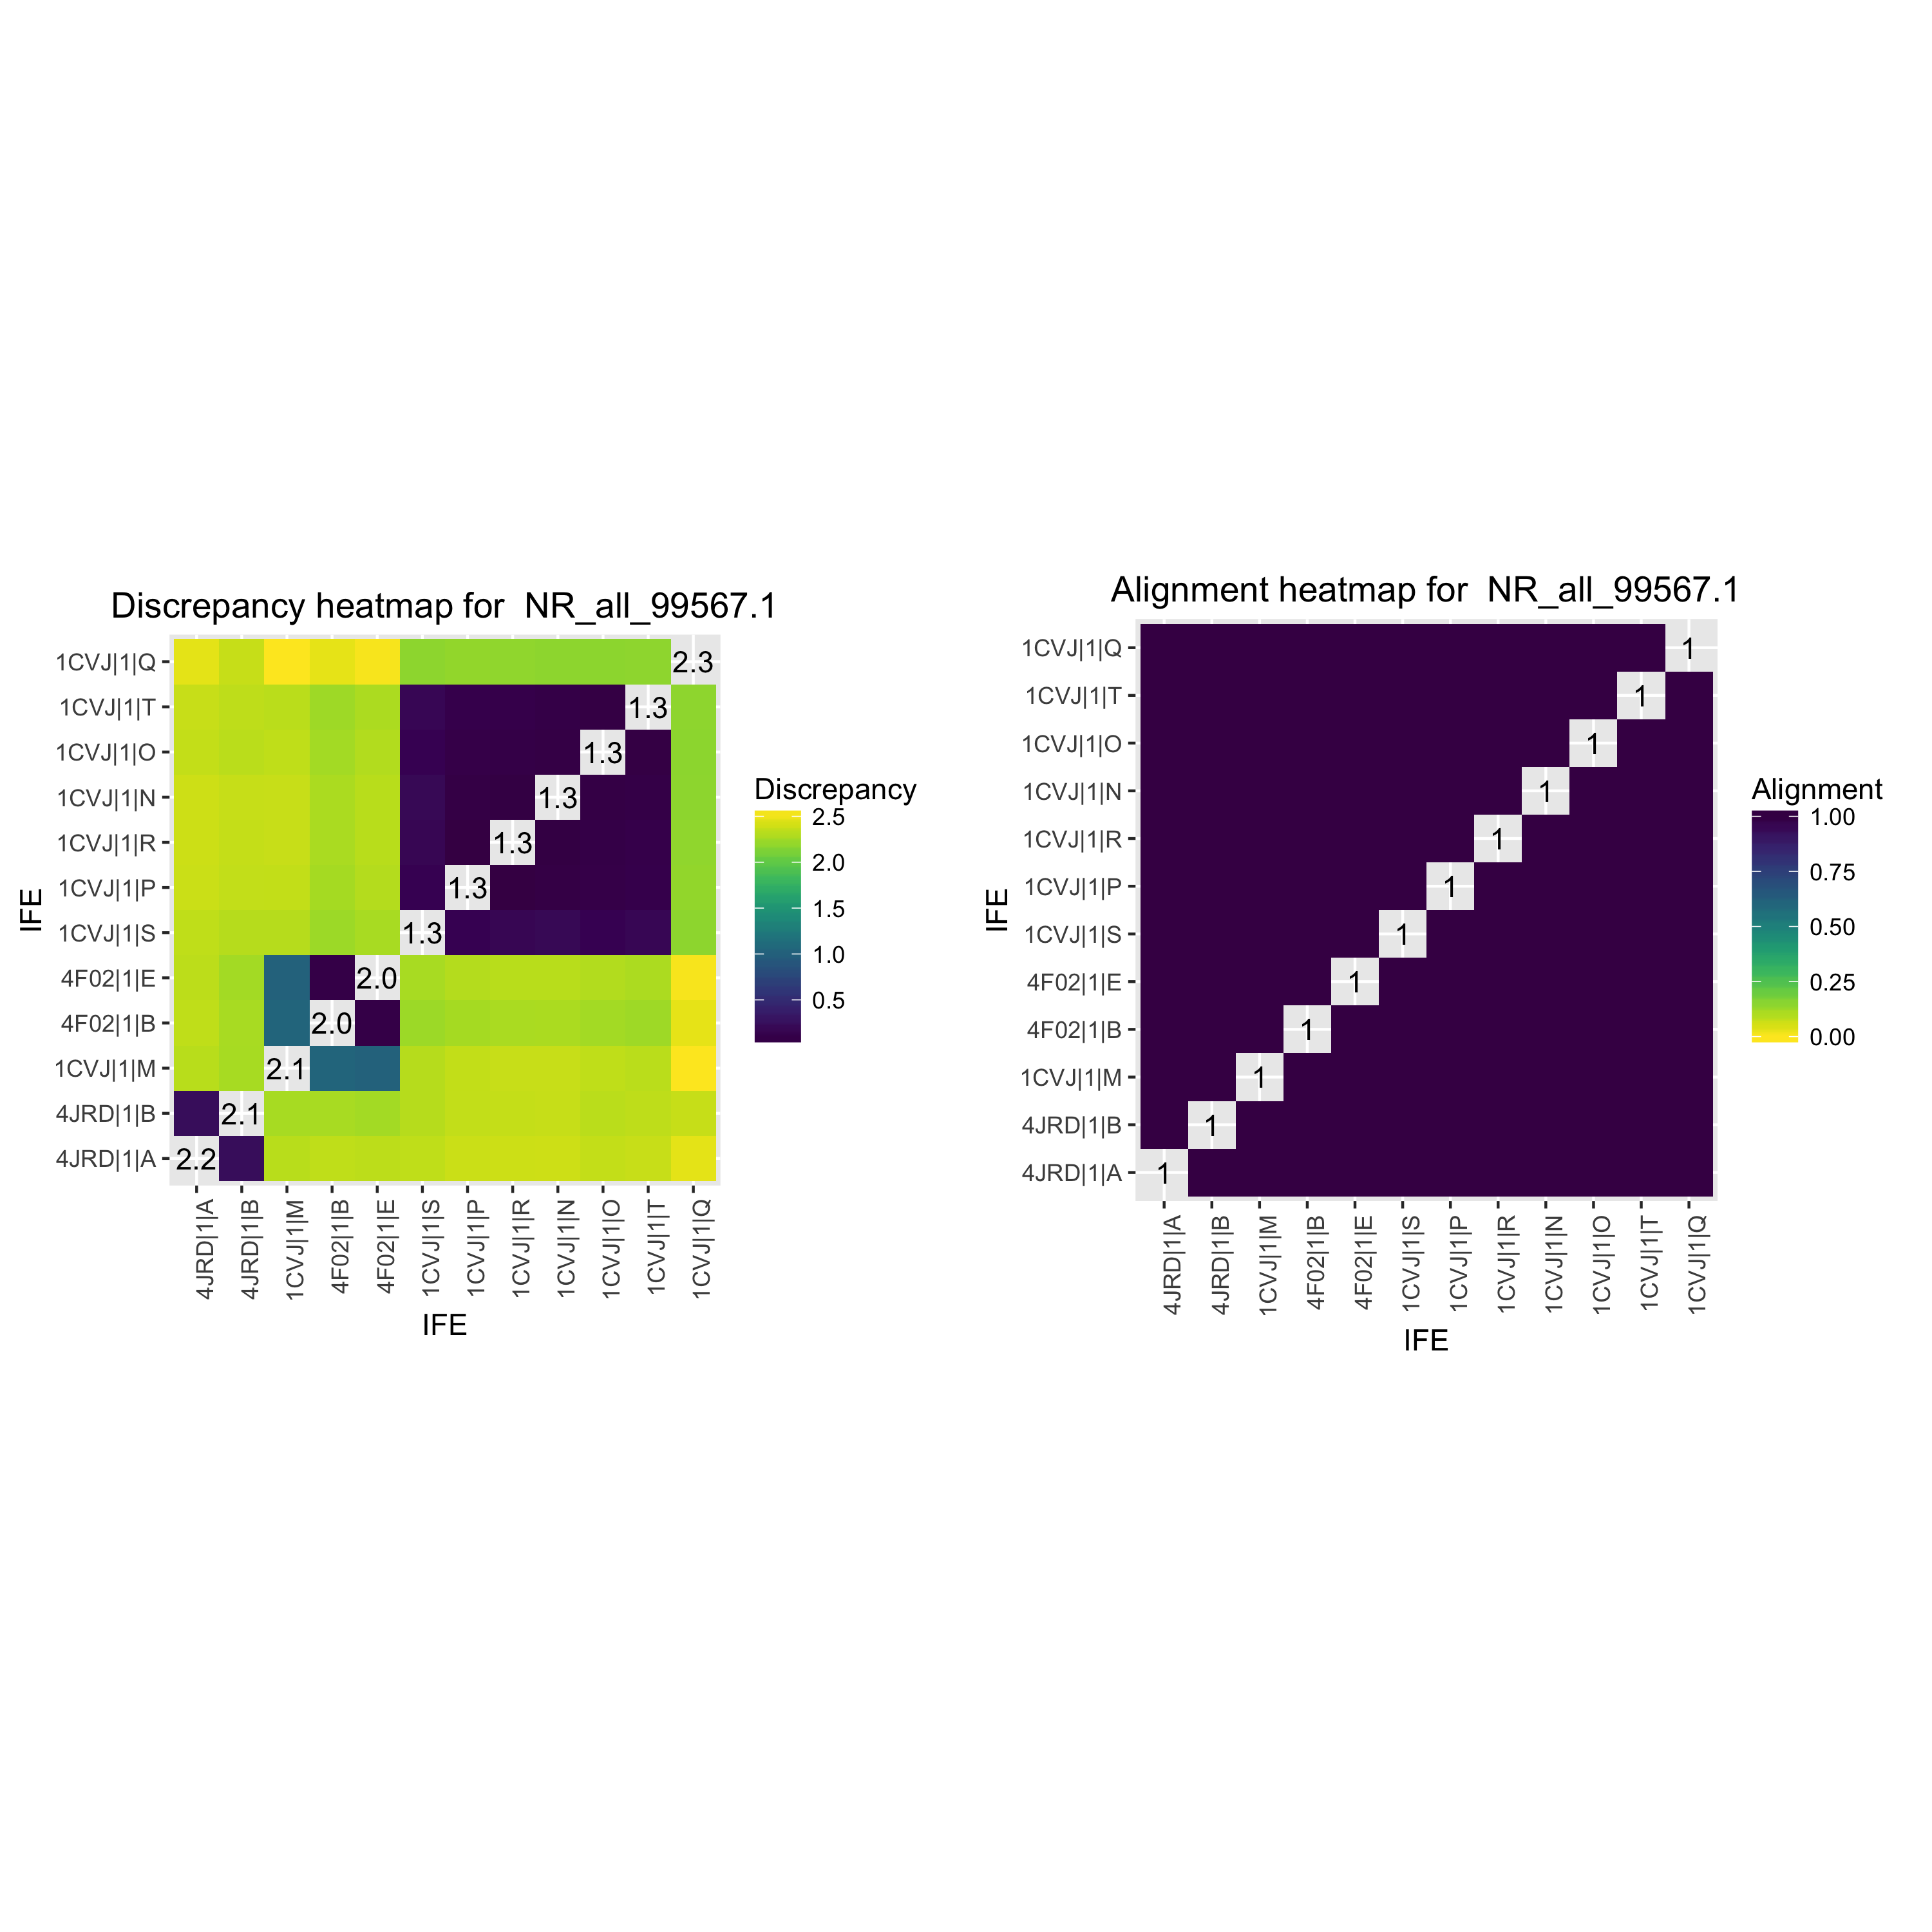
\includegraphics[width=\textwidth]{chapter-3/figs/small-aa-no-disc}
  \caption{Discrepancy heatmap for an 11-nt poly-A class built without
    discrepancy: This shows the effect of clustering a model compound without
    using discrepancy. We are showing only the discrepancy heatmap here. We can
  see that there are several subgroups with very different geometries.}
  \label{fig:small-aa-no-disc}
\end{figure}

\begin{figure}[h]
  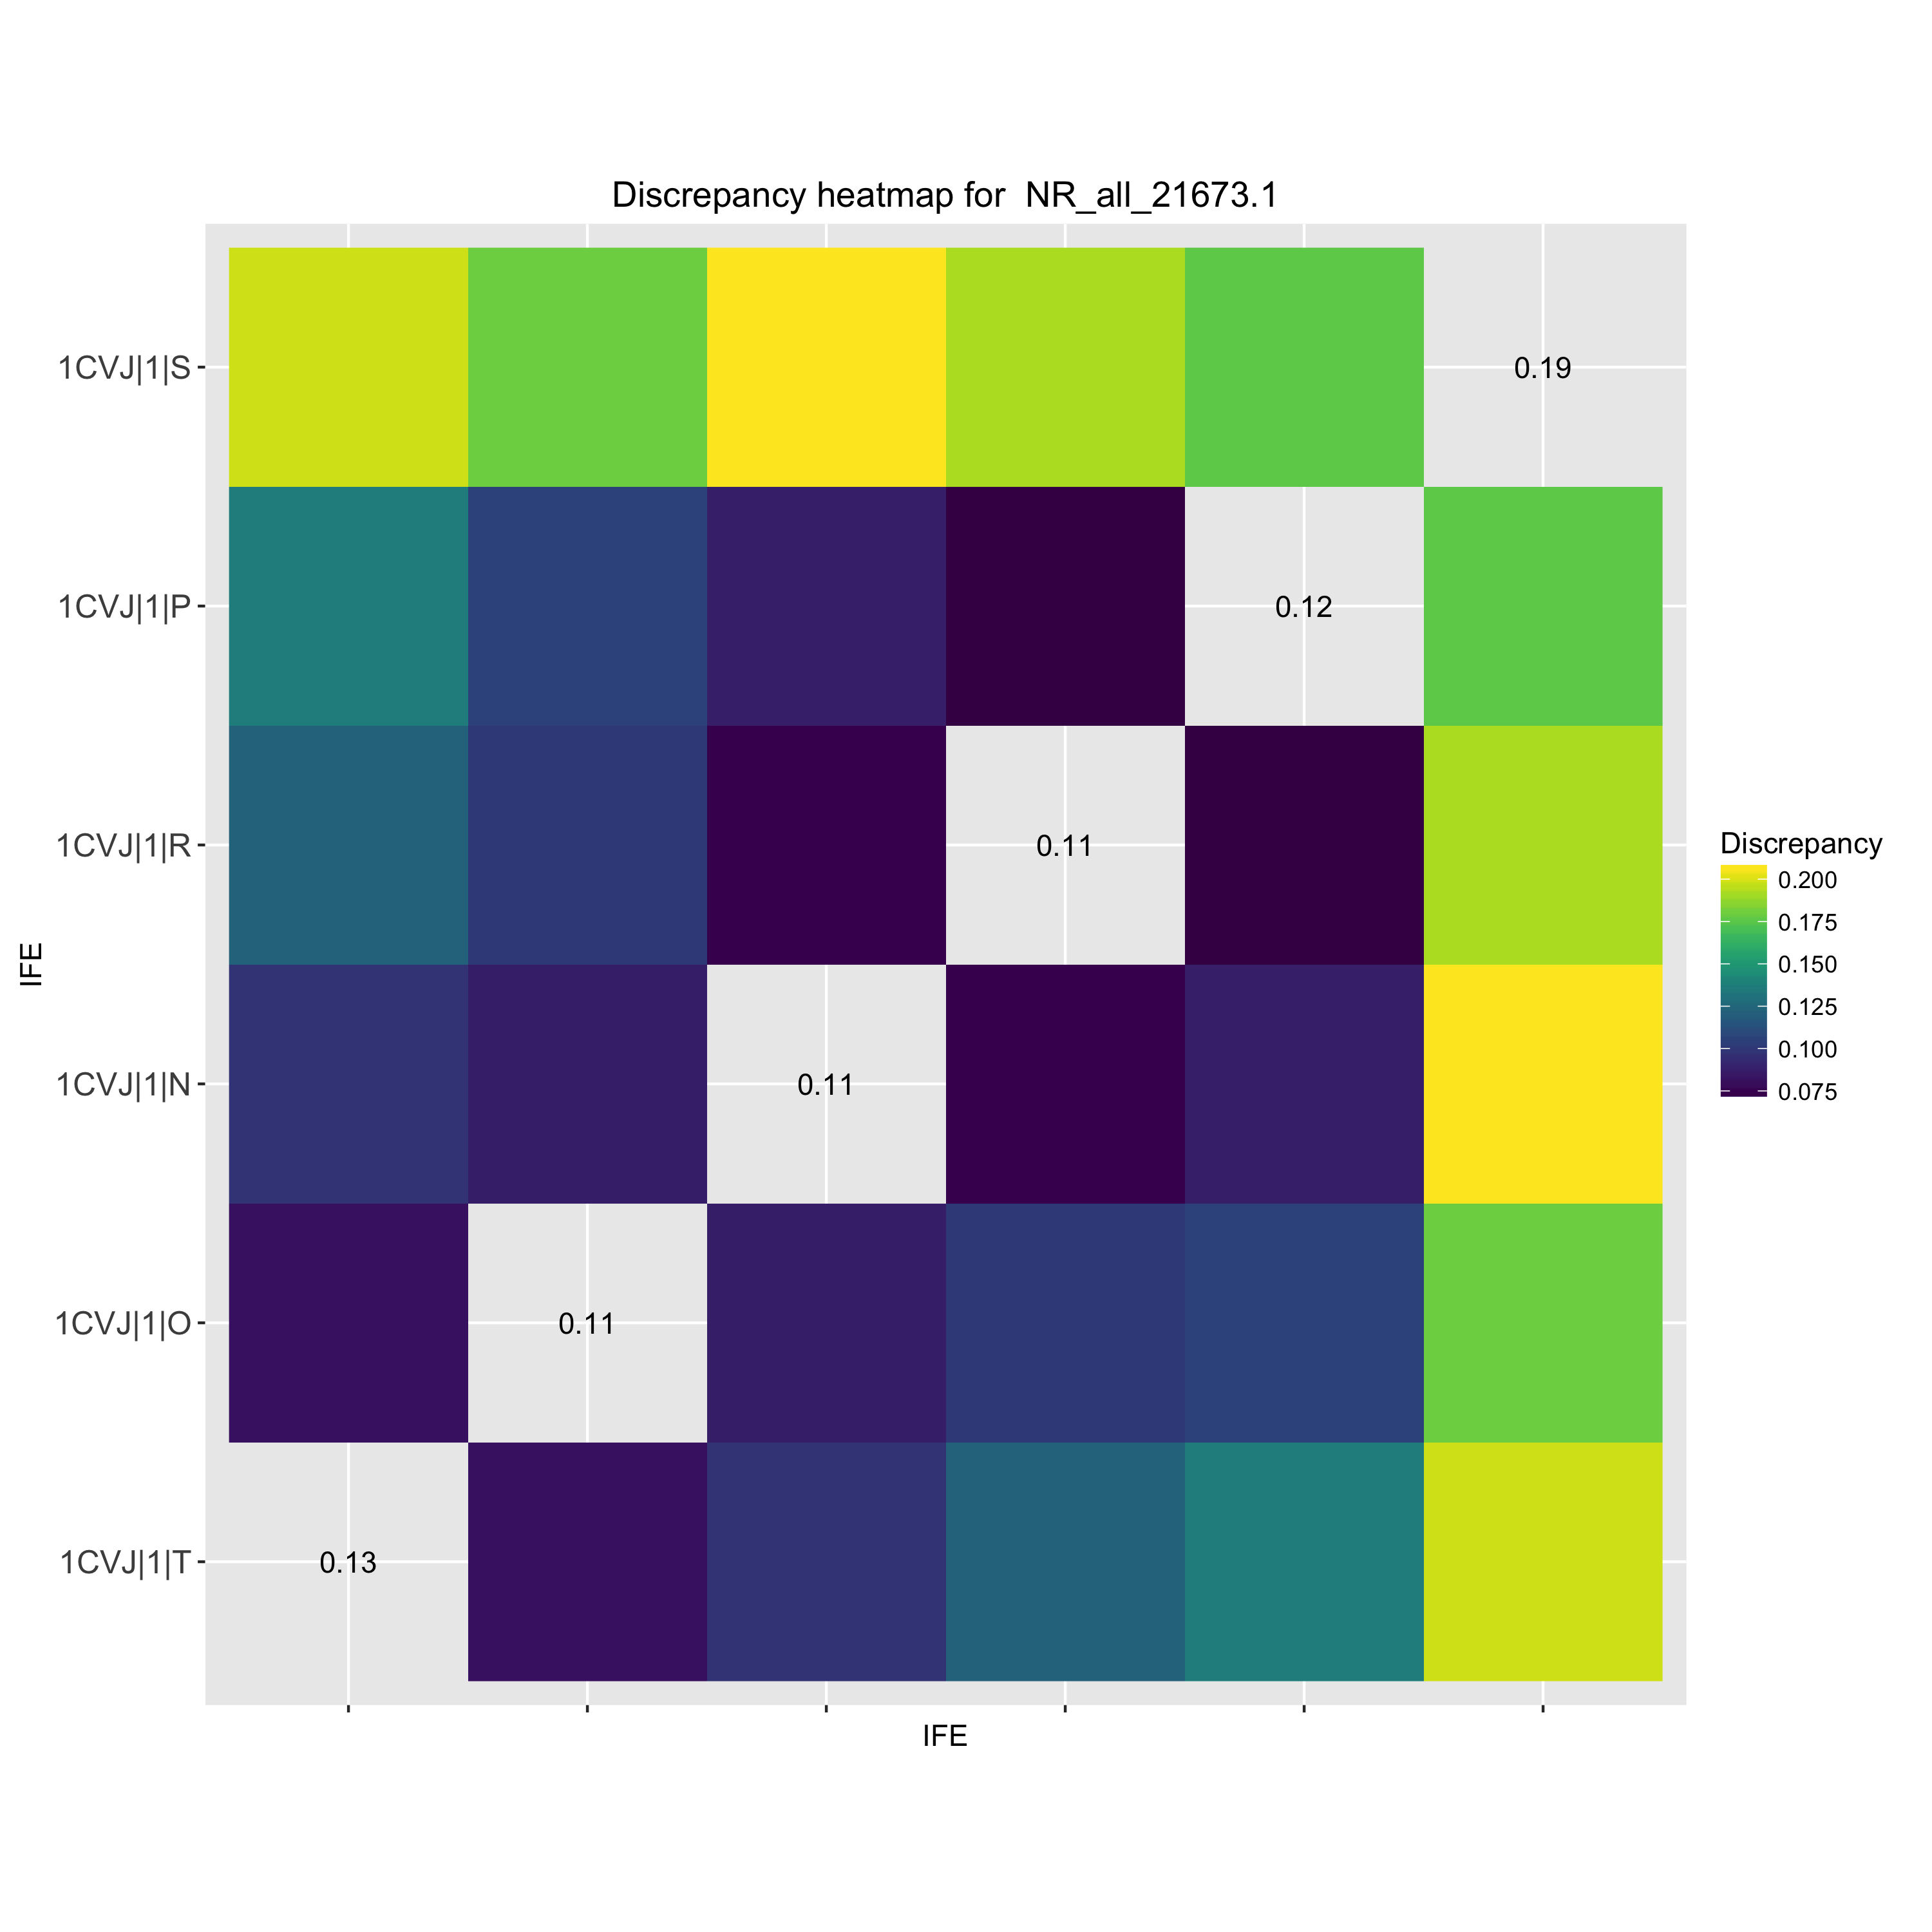
\includegraphics[width=\textwidth]{chapter-3/figs/small-aa-disc}
  \caption{Discrepancy heatmap for a small 11-nt poly-A compound built using
    discrepancy. Mean values for each row are shown on the diagonal, and the
  color scale indicates discrepancy with lighter colors being worse}
  \label{fig:small-aa-disc}
\end{figure}

\subsection{Outliers}

After evaluating specific cases we searched for outliers in our dataset. We
began by examining the distribution of maximum discrepancy and minimum sequence
similarity for all pairs in all equivalence classes. This is shown in in
Figure~\ref{fig:eq-summary}. From this figure we can see that most groups have a low
discrepancy and high sequence similarity. However, there is a very long tail of
groups with high discrepancies, some even ranging up to 4{\AA}/nt. This indicates
that some groups contain pairs of IFE's that are highly dissimilar. We call
these pairs outliers. For the purpose of this analysis we will define groups
with outliers as groups that contain pairs of IFE's with discrepancies greater
than 0.8{\AA}/nt or any group that contains a pair of IFE's that do not have a
‘good’ alignment. As discussed earlier, our criteria for chains to align well
depends on the size of the chains. For this reason we cannot use a simple
sequence similarity cutoff as with discrepancy.

\begin{figure}[h]
  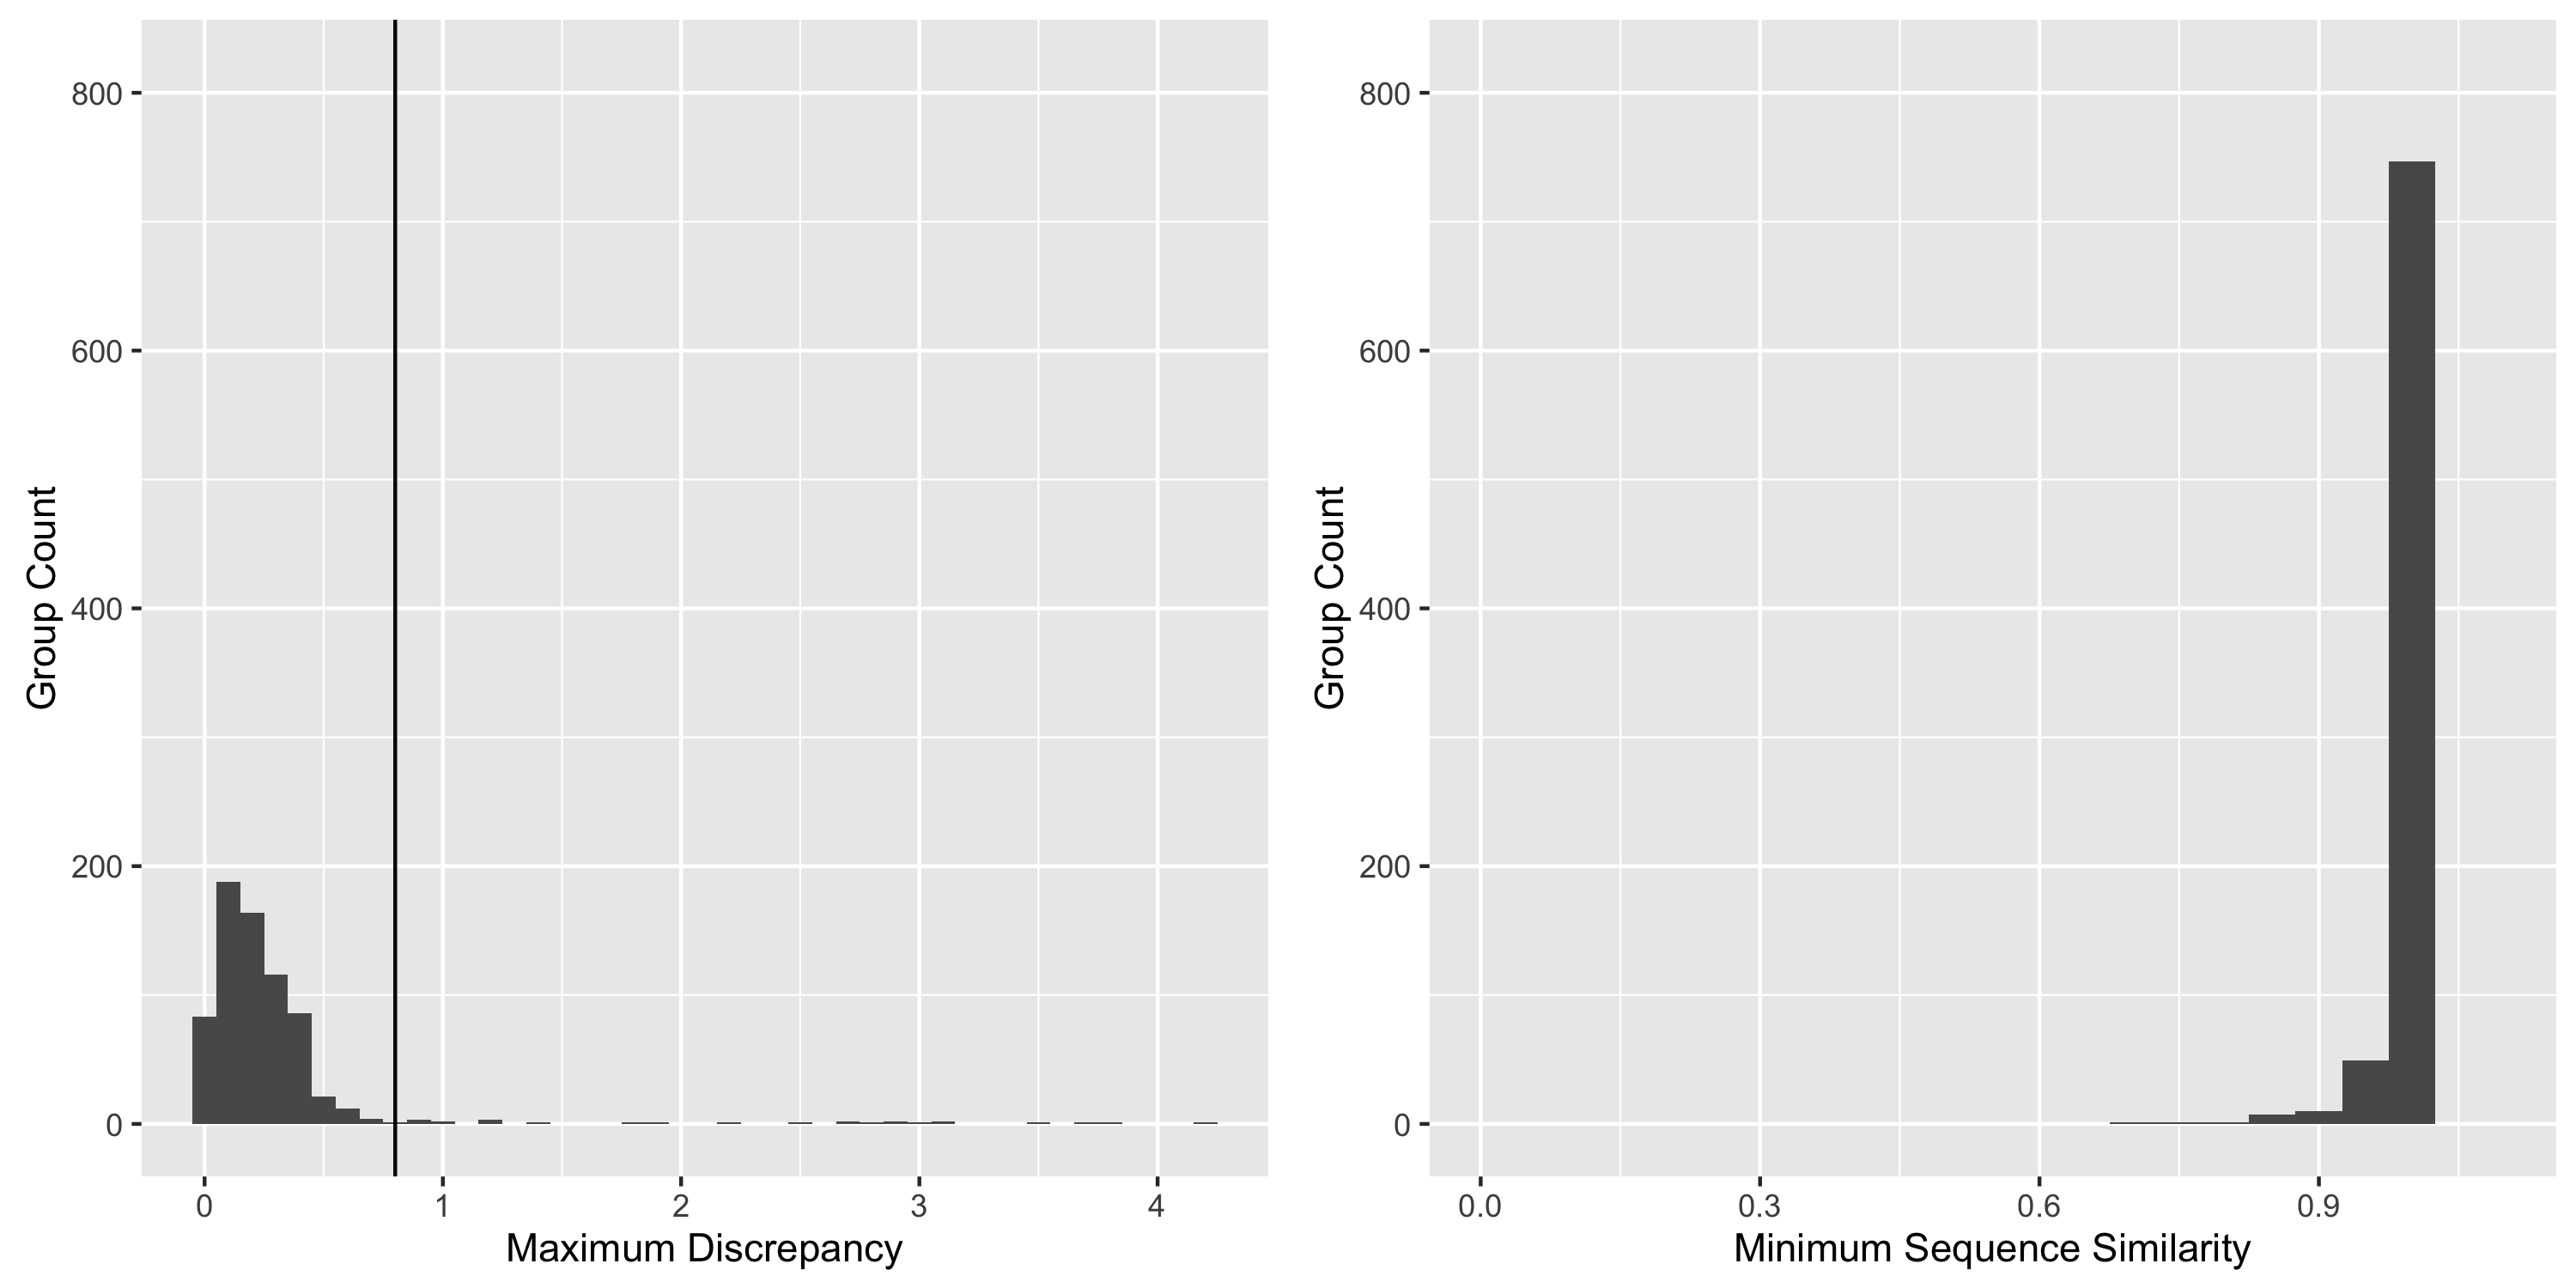
\includegraphics[width=\textwidth]{chapter-3/figs/eq-summary}
  \caption{A figure of the Maximum Pairwise Discrepancy and Minimum Sequence
    Similarity for all pairs of IFE's in all equivalence classes. The black
    lines indicate the 0.8 discrepancy cutoff (left) used a criterion for
  detecting groups with outlier pairs.}
  \label{fig:eq-summary}
\end{figure}

We then investigated the distribution of discrepancies and sequence similarities
for all groups containing outliers. The figuring summarizing this is shown in
Figure~\ref{fig:eq-outlier-summary}. This graph shows that outliers appear in all regions of
the graph. Some outliers have low discrepancy, indicating they must differ in
sequence, while others have high sequence similarity indicating they must differ
geometrically.

\begin{figure}[h]
  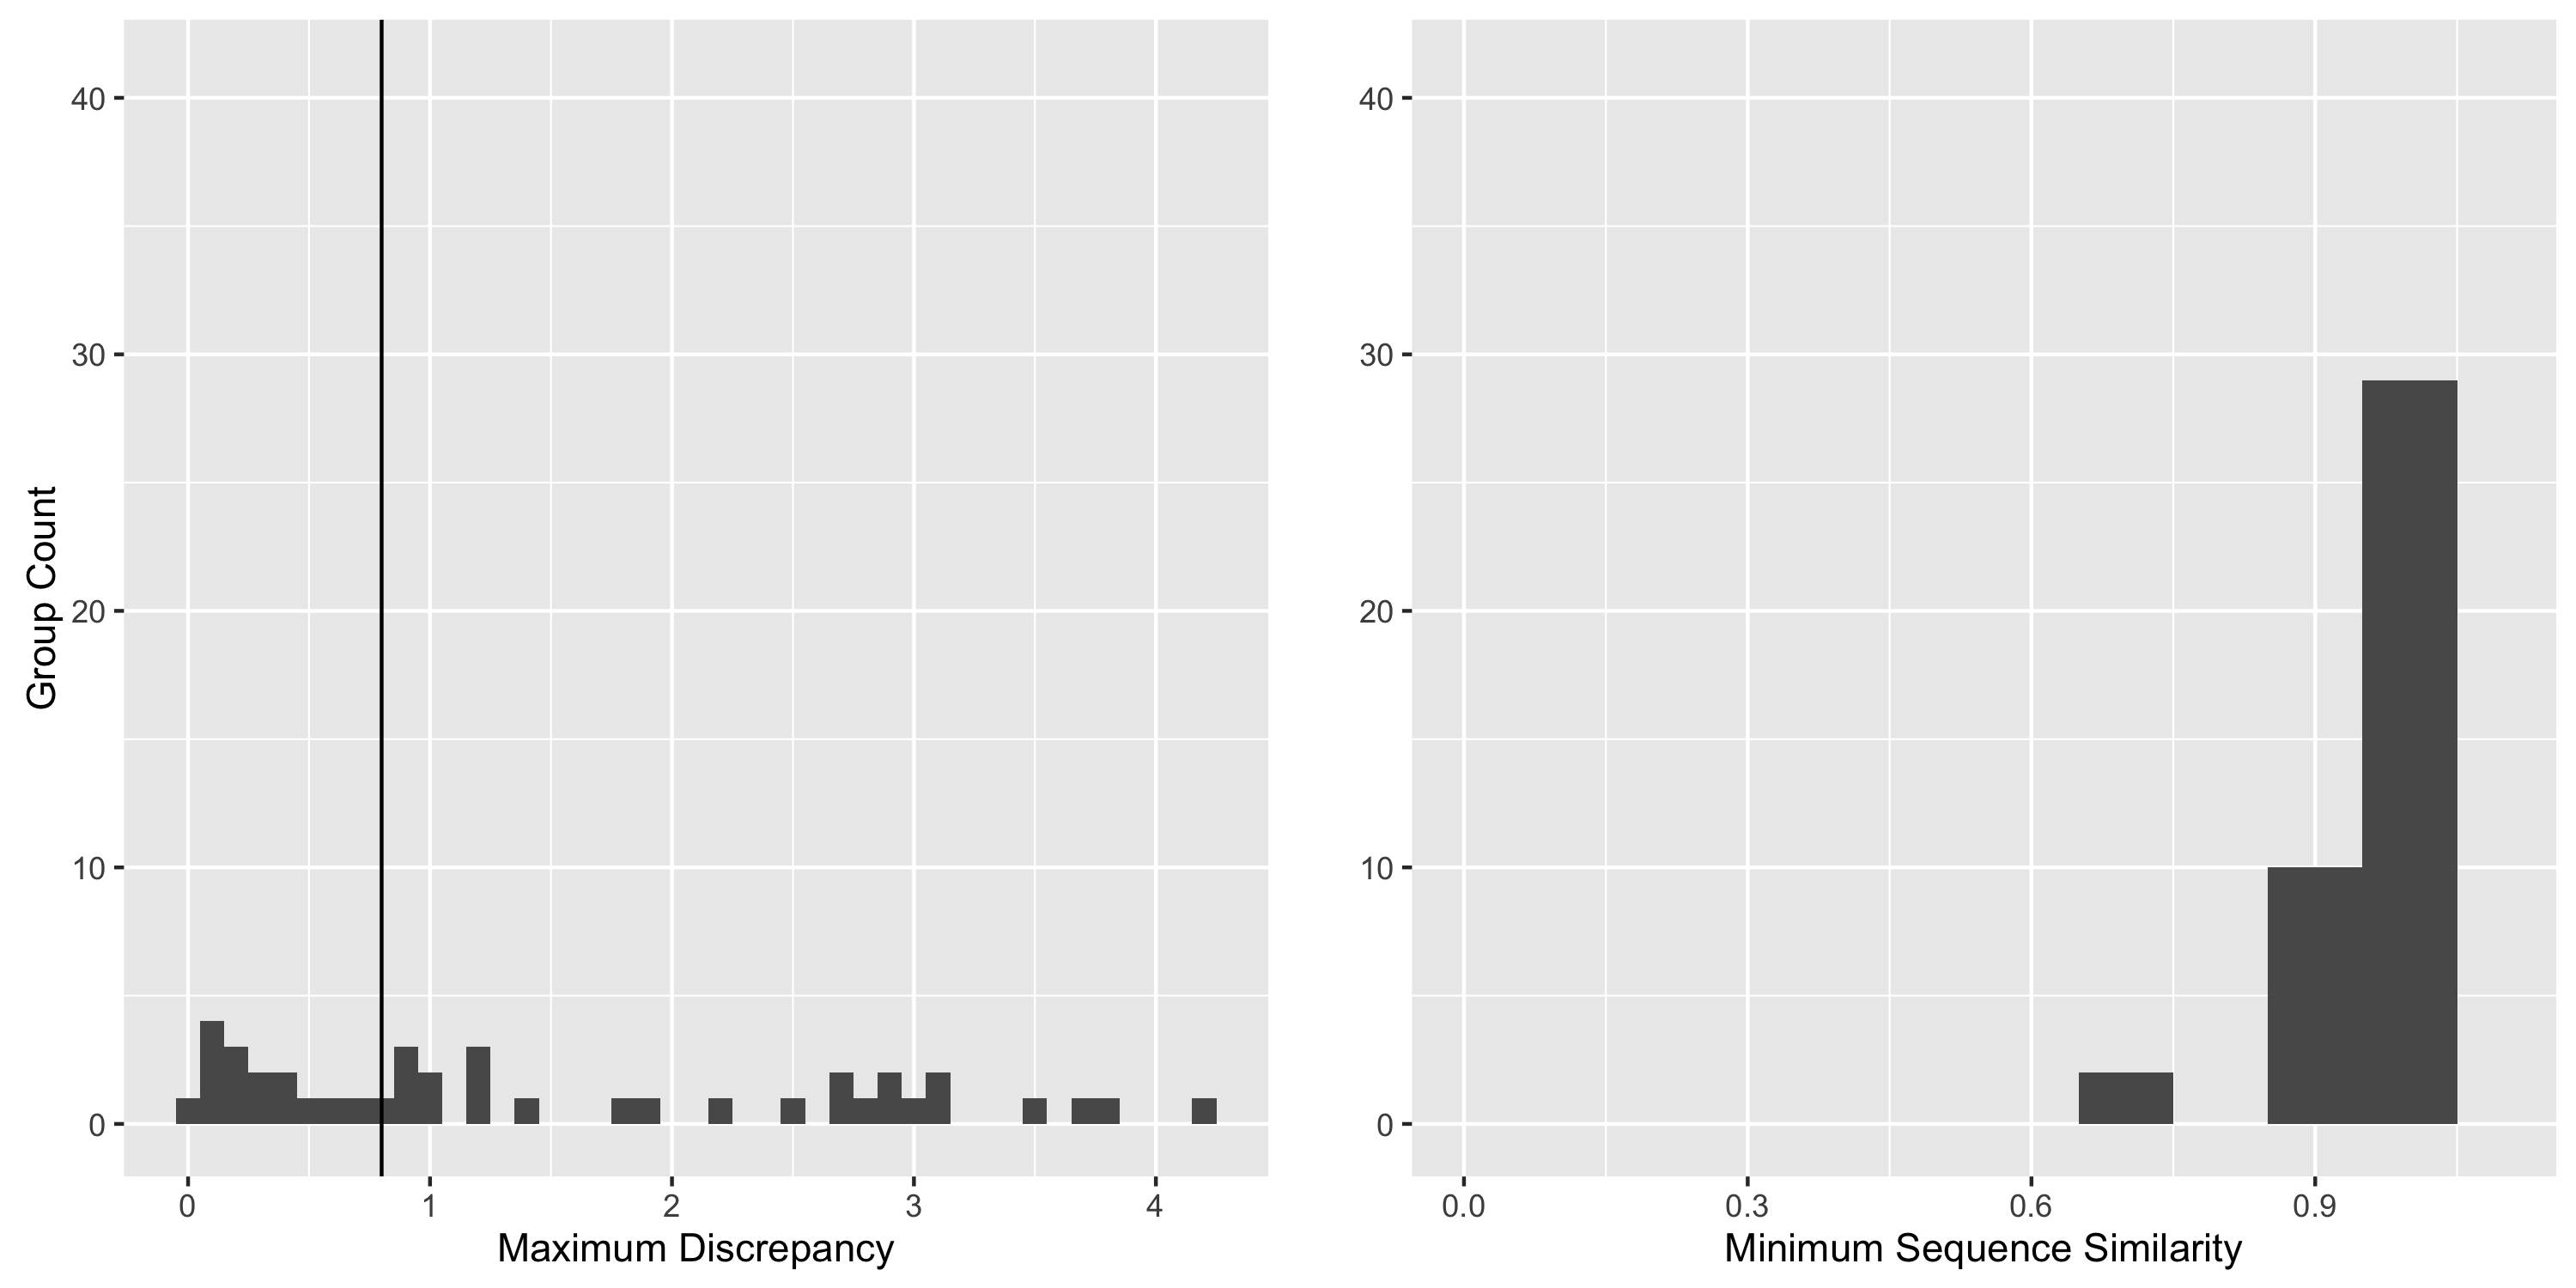
\includegraphics[width=\textwidth]{chapter-3/figs/outlier-summary}
  \caption{Discrepancy and Minimum Sequence Similarity of all groups with
  outliers. This figure shows the same data as Figure~\ref{fig:eq-summary} but
only for groups that have a pair of IFE's with discrepancy at least 0.8 or
sequence similarity less than or equal to 0.9.}
  \label{fig:eq-outlier-summary}
\end{figure}

We next examined the distribution of the number outliers, fraction of outliers,
discrepancy, and sequence similarity with respect to the size of the group in
terms of nucleotides and members as shown in Figure~\ref{fig:outlier-detail}.
This figure shows that the majority of the groups with outliers contain
relatively few members and are relatively small. However, there are a few groups
that contain many members and are large. The spike at \~80 nucleotides
corresponds to 2 tRNA groups.

\begin{figure}[h]
  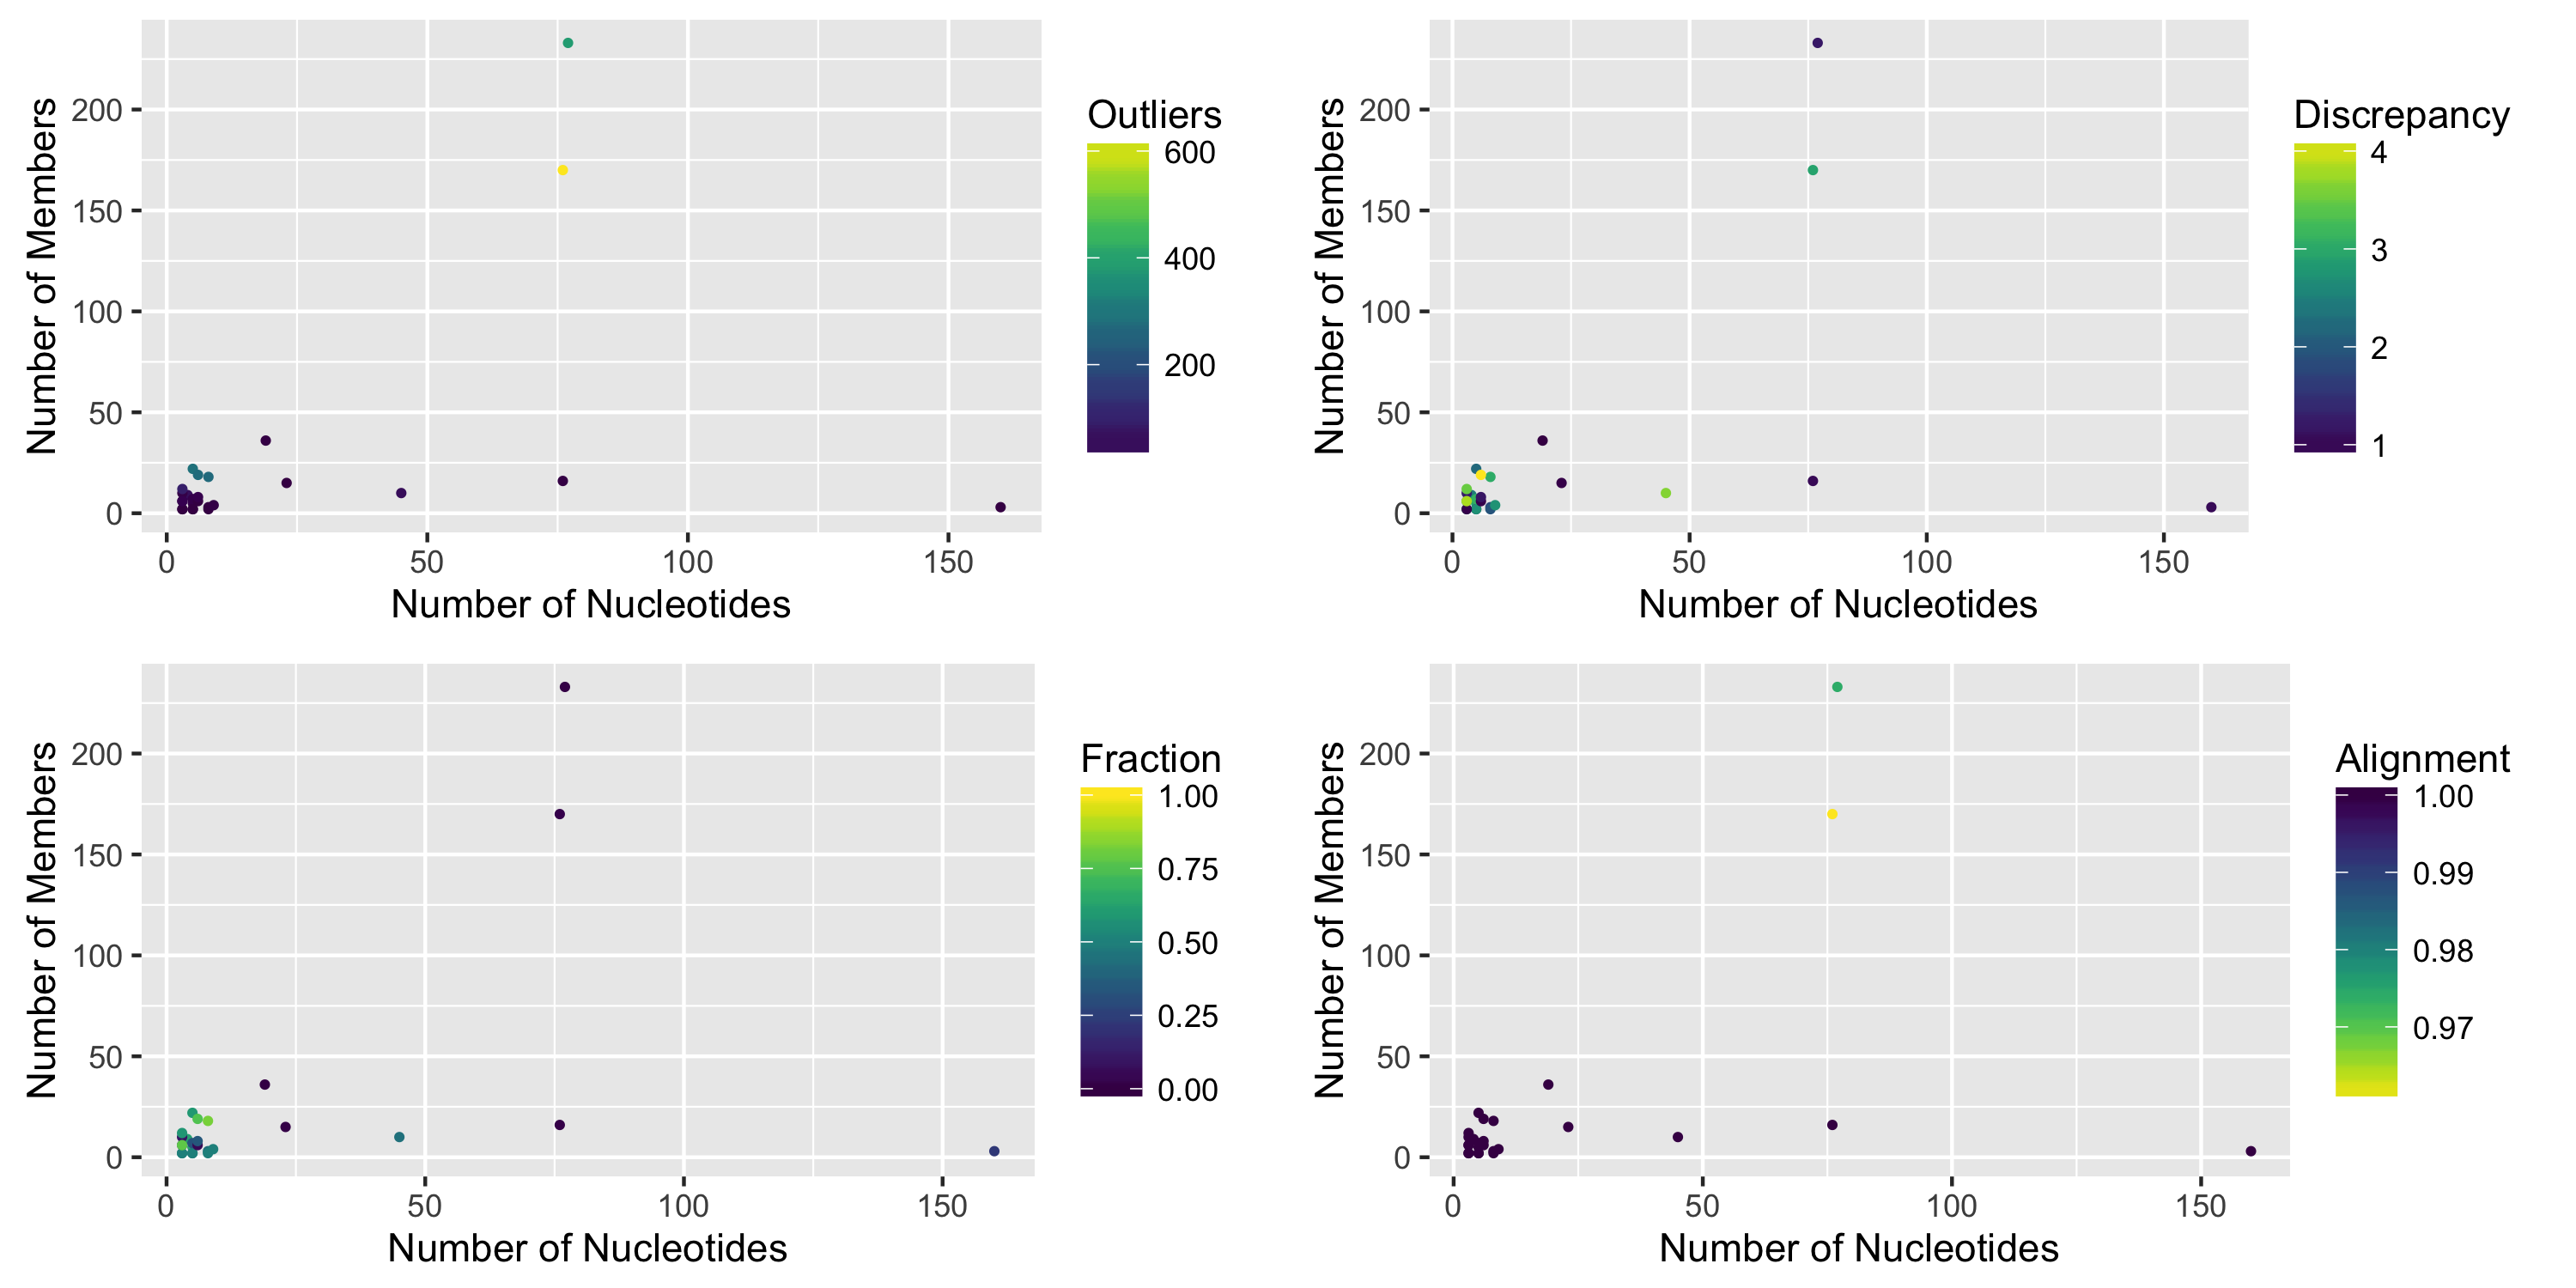
\includegraphics[width=\textwidth]{chapter-3/figs/outlier-details}
  \caption{This figure shows 4 different metrics for outliers within each group.
    Each point in all graphs represents a group that contains at least one pair
    of IFE’s that is an outlier (discrepancy greater than 0.8 or sequence
    similarity less than 0.9). In all graphs the horizontal coordinate is the
    number of nucleotides in the representative (discussed in the next chapter)
    of the group. The vertical is the number of members. The points are colored
    according to various metrics. In the upper right the points are colored
    using the number of pairs that are outliers, with lighter colors meaning
    more. Proceeding clockwise to the upper right the points are colored
    according to the the maximum discrepancy amongst all pairs in the groups.
    The lower right shows the minimum sequence similarity with lighter being a
    lower (worse) score. Finally, the lower left colors the points using the
    fraction of total pairs that are outliers, with lighter being higher
  fraction and thus worse.}
  \label{fig:outlier-detail}
\end{figure}

All groups with outliers can be classified according to the type of of outliers
they contain. The groups may contain pairs that have high discrepancy, low
sequence similarity or both high discrepancy and low sequence similarity. I
determined the counts for each of these as shown in
Table~\ref{tab:outlier-types}. This table shows that the majority of the groups,
63\%, have at least one pair with high discrepancy. The remaining 36\% of groups
contain pairs that have low sequence similarity and no pairs with high
discrepancy. I explored these classes to determine how such groups were built.

\begin{table}
  \begin{tabular}{lr}
    \toprule
    Outlier Type & Number of Groups (Percent) \\
    \midrule
    High Discrepancy & 21 (51\%) \\
    Low Sequence Similarity & 15 (36\%) \\
    High Discrepancy and Low Sequence Similarity & 5 (12\%) \\
    \bottomrule
  \end{tabular}
  \caption{This table shows the counts, and percents, of each type of outlier
  in an equivalence class.}
  \label{tab:outlier-types}
\end{table}

From the definition of our methodology, I know that all groups that contain
pairs with low sequence similarity will do so because they are connected through
a chain of high sequence similarity pairs. The NR\_all\_03381.1 group contains
protein/stem loop constructs of length 22 nt and has 4 members,
\ife{1K8W}{1}{B}, \ife{1ZL3}{1}{B}, \ife{1ZE2}{1}{D} , and 1ZE.

The other class of groups with outliers, those that contain a pair with high
discrepancy, can be caused in two ways. First, the pairs may be connected
through a chain of low discrepancies, similar to pairs with low sequence
similarity being connected through a chain of high sequence similarity pairs.
This is visible in Figure~\ref{fig:nr-all-75770.1-disc}. In this figure there are
yellow bars that only cover part of the

\begin{figure}[h]
  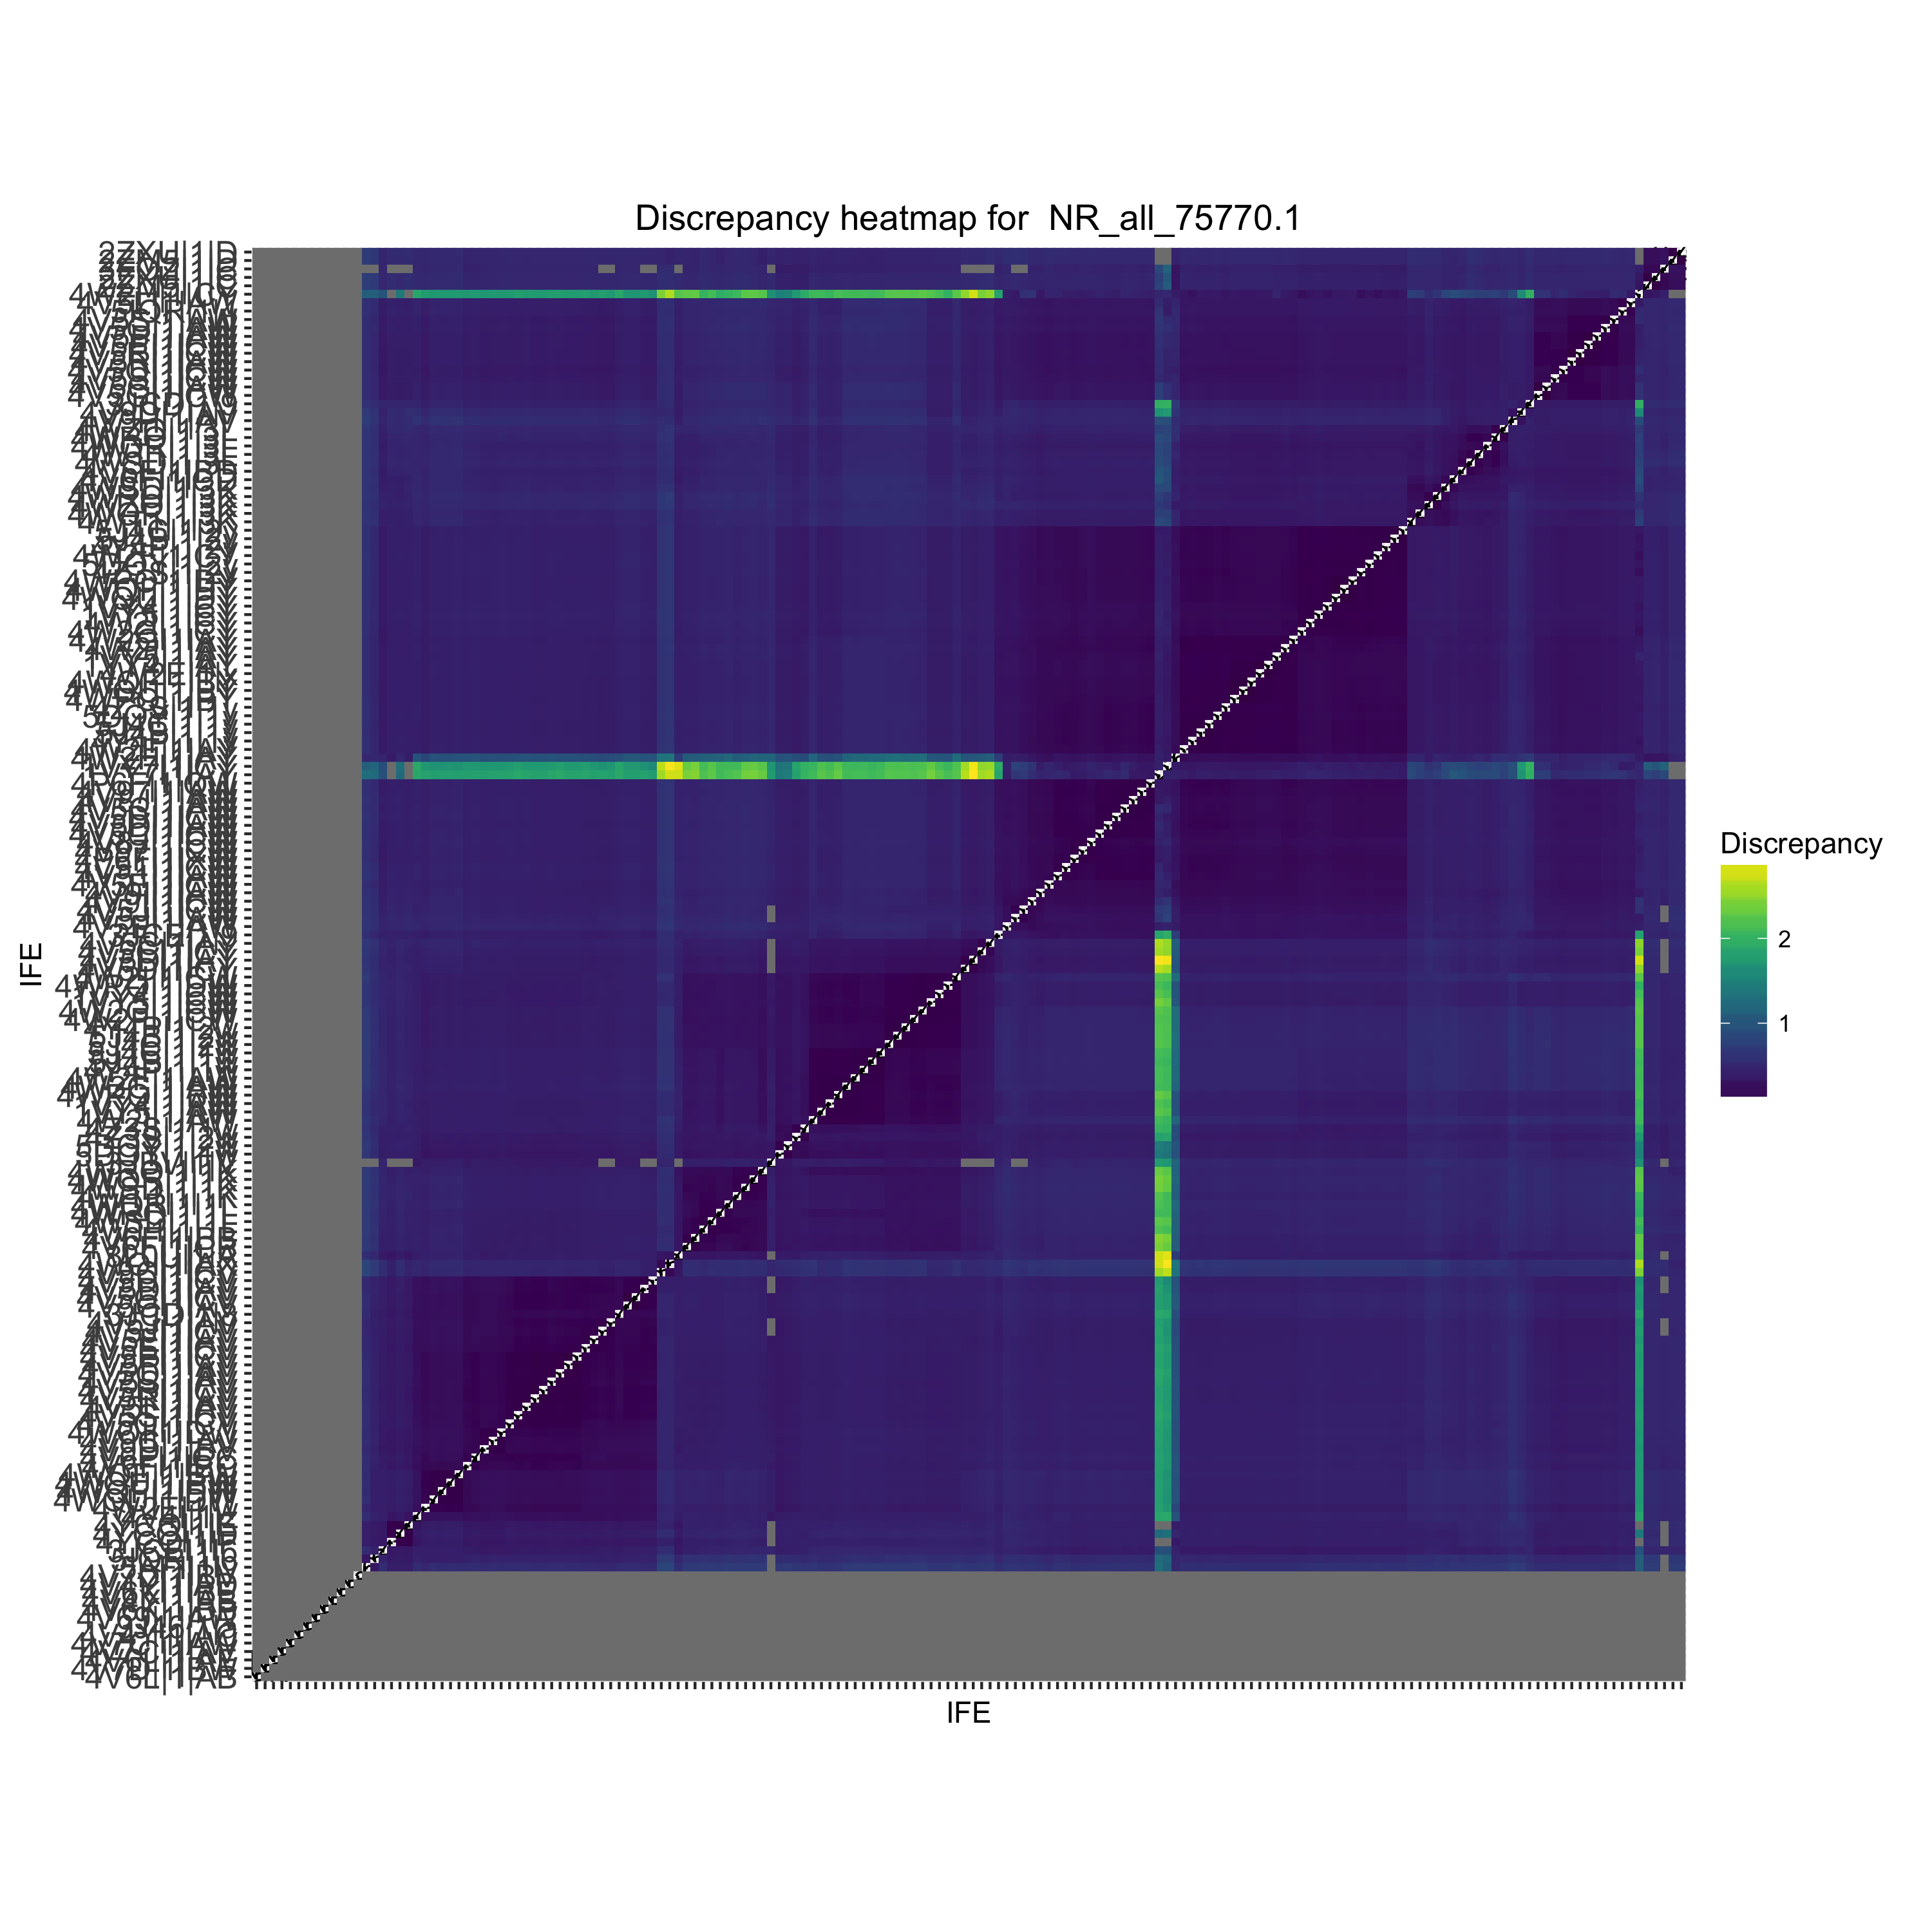
\includegraphics[width=\linewidth]{chapter-3/figs/nr-all-75770-1-disc}
  \caption{Histogram of the of the discrepancies for EC NR\_all\_75770.1, an E.
    coli tRNA group. This group contains a few IFE's which are outliers in our
  analysis.}
  \label{fig:nr-all-75770.1-disc}
\end{figure}

The other possibility is that the chains are connected through an IFE which did
not have discrepancy computed. An example of this is show in NR\_all\_18070.1
DISC. In this figure we can see a yellow line in the upper right which covers
the entire heatmap. This indicates that this IFE has high discrepancy to all
other members of the group. This IFE is connected to all other members through
the IFE’s that have no discrepancy shown (grey bars).

We examined the two groups, NR\_all\_18070.1 and NR\_all\_75770.1 manually and found
that they are tRNA groups. We will look at NR\_all\_18070.1 first, which is a tRNA
group with 233 members and is the highest point on the summary graphs. Shown in
Figure~\ref{fig:nr-all-18070.1-disc}. The outliers are due to a single IFE which is a
truncated tRNA. While it is somewhat structurally different from all other
members it is very similar in sequence. Because these molecules are uncommon and
it is still similar enough to rest of the group to ‘belong’. It is connected to
the rest of the chains through IFE’s which have no computed discrepancy.

\begin{figure}[h]
        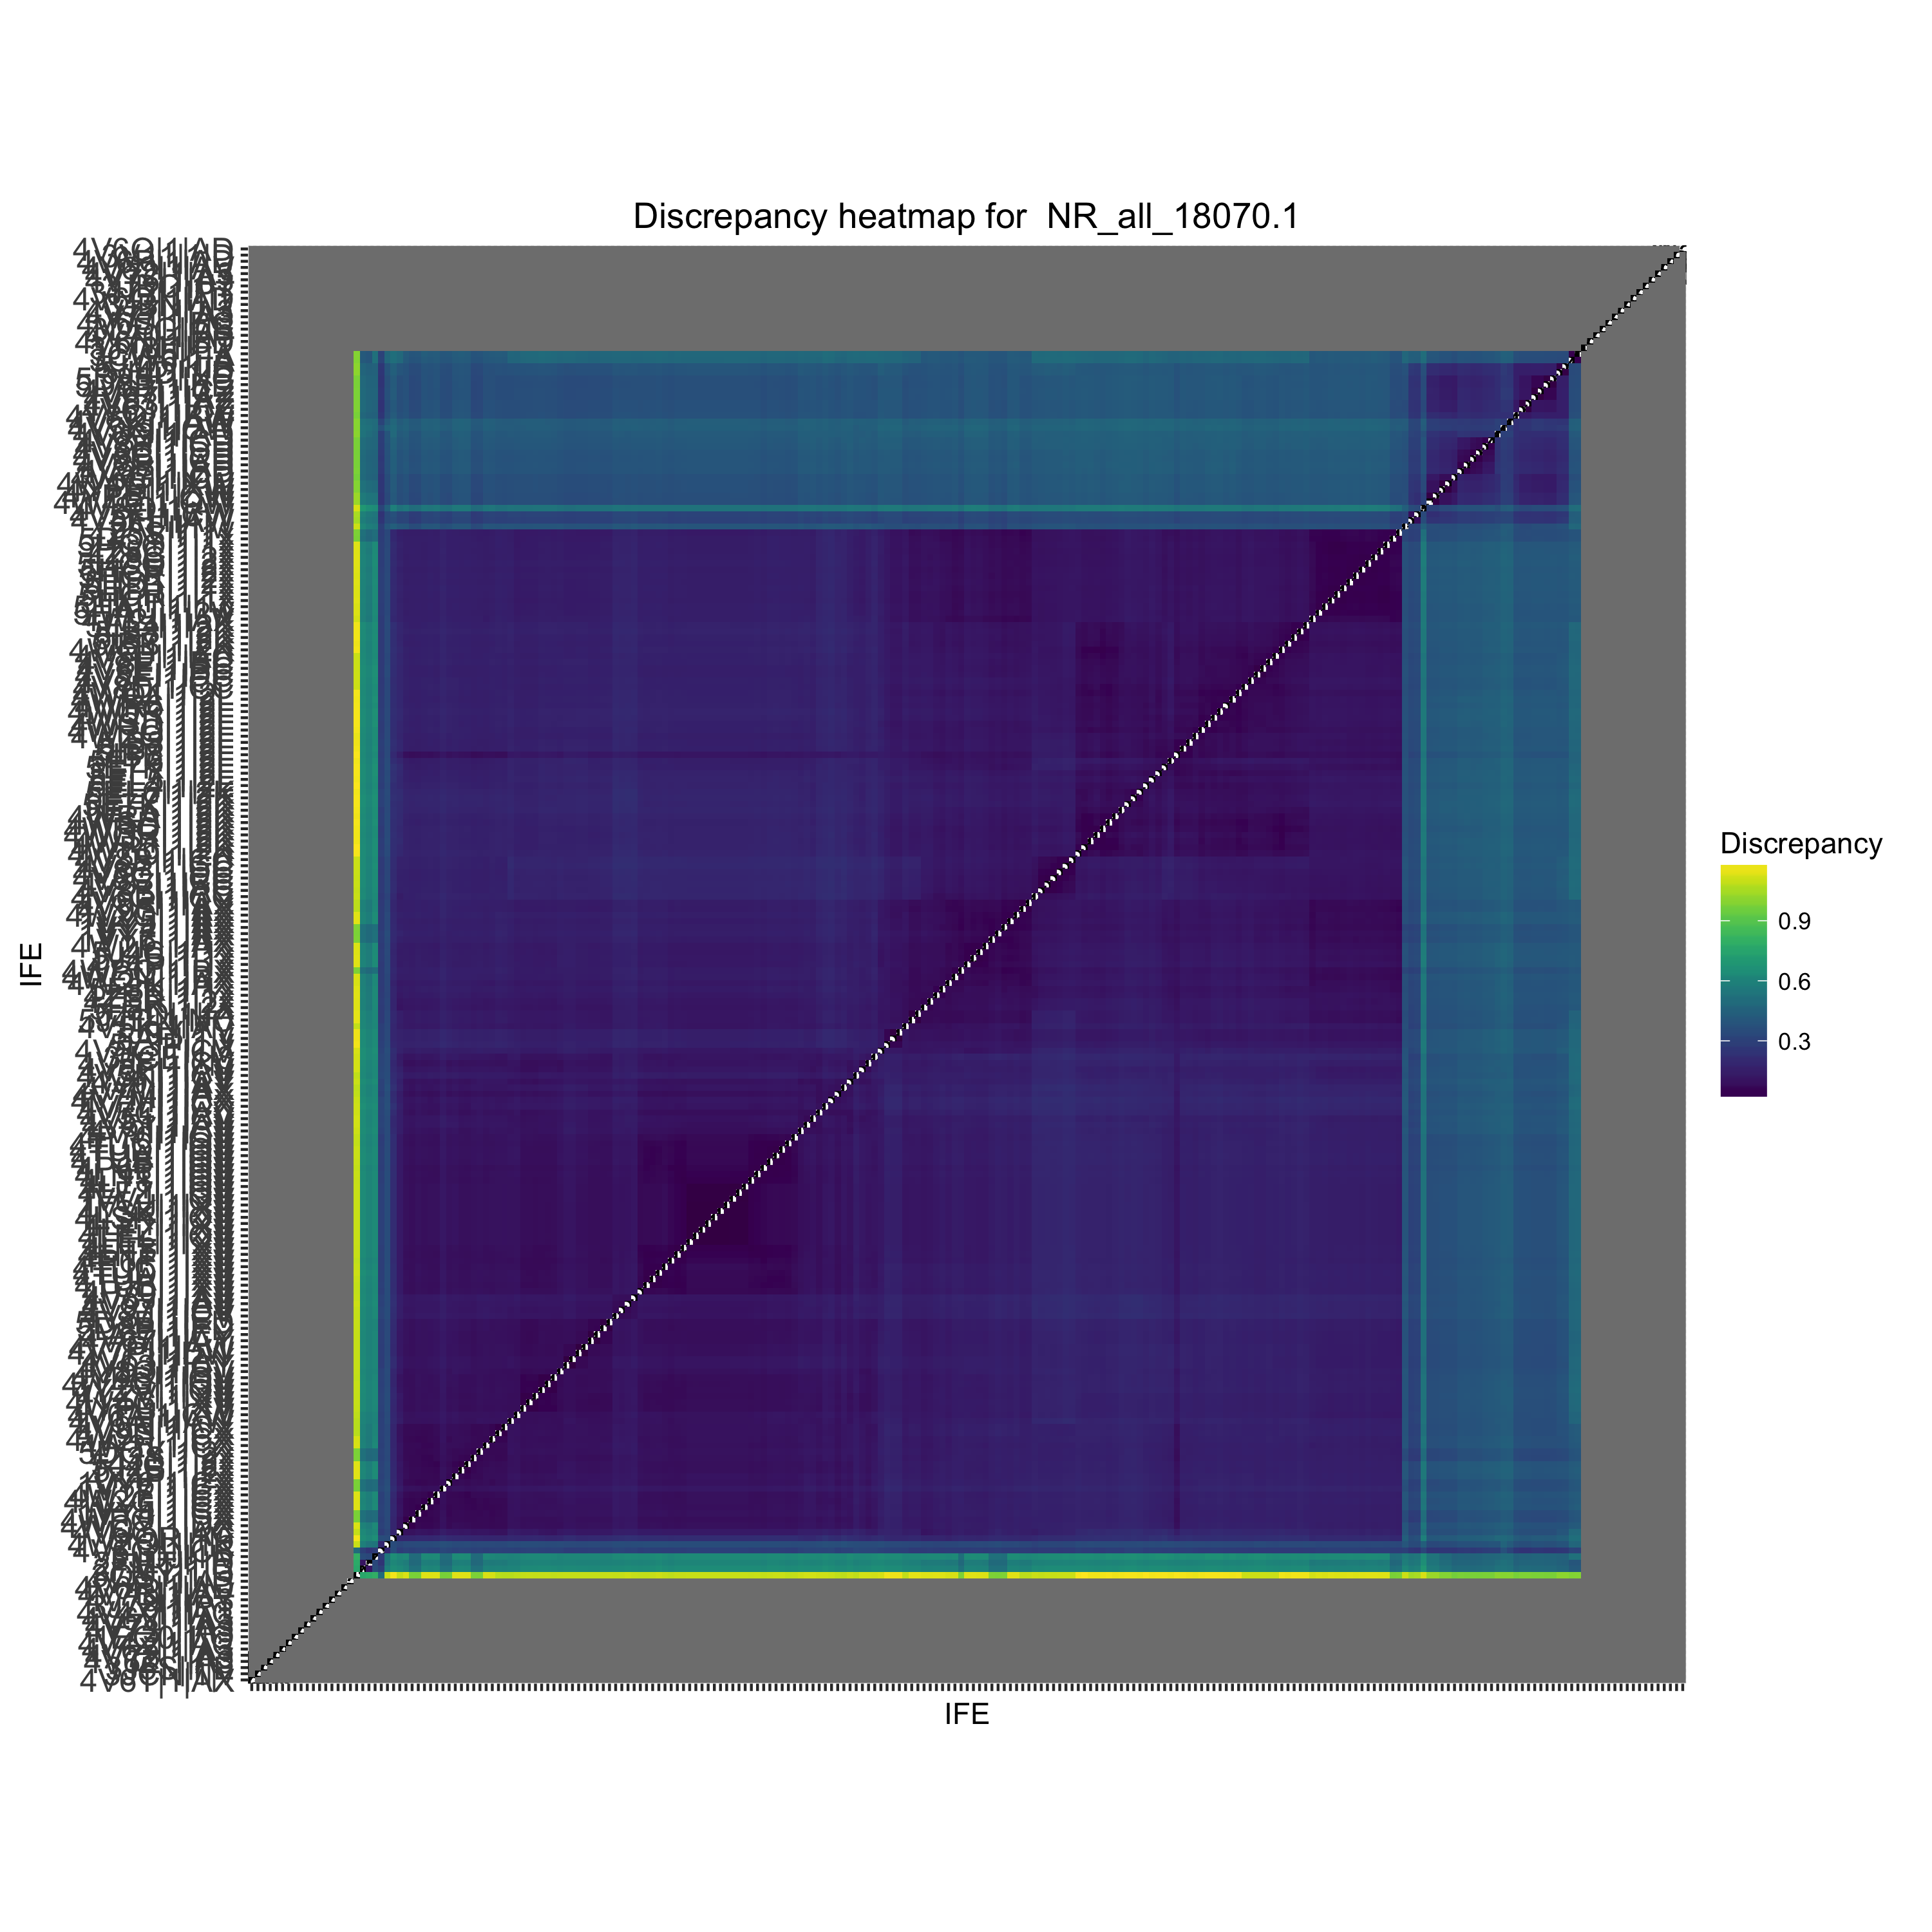
\includegraphics[width=\textwidth]{chapter-3/figs/nr-all-18070-1-disc}
  \caption{Figure summarizing the discrepancy heatmap for all IFE’s in
  NR\_all\_18070.1, a tRNA group with 233 members. }
  \label{fig:nr-all-18070.1-disc}
\end{figure}

The second NR\_all\_75770.1 is the second highest point on these plots. It is an
E. coli tRNA group with 170 members. There are a few IFE’s which are outliers
relative to the rest of the group. These chains appear to be fragments of the
larger tRNA. For example 1VY7 is a 5 nt fragment of the 76 nt tRNA.

We manually investigated the other groups with outliers and found that the
outliers are often placed into the same group because there is a structure that
we do not compute discrepancy for, such as a low resolution X-ray, that connects
the outliers to the rest of the group. For example, in previous version where we
did not compute discrepancy for NMR structures, an HIV hairpin would get joined
with a duplex of the same sequence because there was a NMR structure. All three
types of chains, the duplex, hairpin and NMR structure contained the same
sequence and thus were joined on the basis of sequence similarity. This was
resolved for NMR structures with the usage of discrepancy for them as well.
However, it remains an issue for low resolution X-ray and crystallography
experiments.

\section{Conclusions and future extensions}

Overall our grouping methodology successfully groups all chains into equivalence
classes. Our methodology is an improvement over the previous approach for
several reasons. First, it can work with mmCIF data by not only cluster the
largest chain in a file. Secondly, it computes and all discrepancies and
alignments to allow for future tuning of the parameters. Finally, our method
does not compute discrepancies for low resolution structures which will show
artificially high values.

There are several improvements that should be made. Notably, our method of
geometric similarity, discrepancy, is flawed for this task. It is too sensitive
to poor modeling in structures. Often the issue is the bases in nucleotides have
unusual orientations. If this was replaced with a different method that is less
sensitive to base orientation it may be possible  to compute all geometric
comparisons.

In addition, while evaluating the methodology it has been very useful to compute
a grouping using only sequences and then examine the changes when discrepancy is
applied. This could become part of the standard clustering procedure. For
example it may be useful to create a series of groupings built off each other.
The first a simple sequence only building, then adding species constraints, then
finally adding the discrepancy comparisons. This would make it easier to examine
our methodology as well as provide information about the linkages, if any
between groups. For example, there are likely many small groups that differ
structurally but have the same, or very similar sequences. Such groups may be
interesting for researchers interested the range of structures a single sequence
can form. A hierarchy of groupings could make this easier to determine.

Finally, small structures may well require a different set of rules for
comparison grouping. The work here was guided strongly by our experience with
ribosomes and tRNA molecules. These are much larger and show much clearer
differences than small synthetic molecules. It may be worthwhile to focus
exclusively on the small molecules to improve the methodology. For example, we
currently only use one chain when making geometric comparisons. This works well
with large molecules buy may not be accurate for small synthetic compounds. In
addition, it may be better to allow small chains to join through non-canonical
pairs as well as canonical cWW pairs. Doing so could allow us to build better
groups for the poly-A duplex or G-quadruplexes more accurately.

\chapter{SELECTION OF THE REPRESENTATIVE SETS FROM THE EQUIVALENCE CLASSES OF
RNA CONTAINING 3D STRUCTURES}

\section{Introduction and motivation}

The previous chapter discussed a method for organizing all RNA-containing 3D
structures in PDB into sets of equivalence classes. This procedure structures
the 3D dataset. However, for many use cases, simply organizing the data is
insufficient. In particular studies exploring the statistical properties of the
structural data set will be biased toward 3D structures that are highly
represented, as is currently the case with tRNA and ribosome structures. A
summary of is shown in Table~\ref{tab:mol-dist}.

\begin{table}
  \begin{tabulary}{\linewidth}{LRR}
    \toprule
    Molecule &
      Number of Integrated Functional Elements in the class &
      Percent of all RNA containing structures in PDB as of Sept 09, 2016 \\
    \midrule
    \TT{} LSU            & 282  & 4.0 \\
    \TT{} SSU            & 379  & 5.4 \\
    \TT{} 5S             & 282  & 4.0 \\
    \EC{} LSU            & 161  & 2.2 \\
    \EC{} SSU            & 157  & 2.2 \\
    \EC{} 5S             & 156  & 2.2 \\
    \HM{} LSU            & 69   & 0.9 \\
    \HM{} 5S             & 67   & 0.9 \\
    \DR{} LSU            & 42   & 0.5 \\
    \SC{} SSU            & 56   & 0.8 \\
    \SC{} LSU            & 63   & 0.9 \\
    Other Ribosomes      &      & \\
    Ribosomal Subtotal   & 1714 & 24.5 \\
    Remaining Structures & 5287 & 75.5 \\
    Total                & 7001 & 100 \\
    \bottomrule
  \end{tabulary}
  \caption{Proportion of solved structures that are from bacterial and yeast
    ribosomes. This table shows data from the 2.92 release of NR set at the
    'all' resolution, availabe at:
    \url{http://rna.bgsu.edu/rna3dhub/nrlist/release/2.92/all}. This dataset contains
    all structures available as of Sept 09, 2016. This table presents the
    fraction of the total structural database that comprises structures from all
    sources ribosomes. In total they make up 20\% of the solved crystal
  structures. LSU: Large Ribosomal Subunit, SSU: Small Ribosomal Subunit.}
  \label{tab:mol-dist}
\end{table}

As seen in the table, \EC{} and T. thermophilus ribosomes alone make up 20% of
the entire dataset and all ribosomal total NNN. For many statistical analyses of
RNA structure, it is desirable to identify one high quality representative
structure \cite{Leontis2012b}. For example, such a reduced redundancy dataset
set is desirable for constructing the RNA 3D Motif Atlas \cite{Petrov2013}. In
previous work a method to identify representative structures  from PDB format
files, called the non-redundant (NR) set was developed. We have updated the
method to take advantage of the new mmCIF data and fix limitations of the
previous method. These were posted on a weekly basis from February 5, 2011 to
December 5, 2014 on the BGSU RNA site and made available for searching on NDB
(\url{http://ndbserver.rutgers.edu/}).

\section{Requirements for representative set}

The set of representative structures has a variety of uses in structural
bioinformatics applications. Most notably it supports population and regular
updating of the RNA 3D Motif Atlas \cite{http://rna.bgsu.edu/rna3dhub/motifs}.
The RNA 3D Motif Atlas is a clustering of all high quality loops extracted from
all structures in the current Representative Set of structures. For this reason
it is desirable to avoid frequent changes in the representative structure due to
insignificant increments in the selection criteria. If we allow frequent
insignificant changes in the representative in structures selected for the
Representative set, these changes cause large changes in the RNA 3D Motif Atlas.
This makes the resource appear more unstable than it actually is and so we aim
to avoid changes due to minor improvements in structures. Thus the goals are of
the improvements described in this chapter are:

\begin{enumerate}
  \item The representative set should reflect observed variation in sequence,
    structure, and biological variation in the set of solved 3D structures

  \item The representative set should contain highest quality representative
    X-Ray structures from each Equivalence Class. NMR or Cyro-EM structures are
    chosen as representatives only when no X-ray structure is available.

  \item The representative set should only change upon the appearance of new,
    significantly better structures, using criteria explained in this chapter.
\end{enumerate}

The representative set is intended to display the observed structural, sequence,
and biological variation present in the current RNA-containing structural
dataset, avoiding duplication as much as possible. Each unique structural class
should be represented by one high quality structure, as the classes already take
into account the possibility of large structural variation, as explained in the
previous chapter. It is desirable to pick the highest quality structure
available from each equivalence class. A high quality structure is one that
models the experimental data as well or better than other available structures
and is as complete as possible.

\section{Methodology for selecting representative RNA 3D structures from
Equivalence classes}

This dissertation describes new methodology that represents significant
improvements over the previously developed methodologies of the BGSU RNA
resource. In the previous method, the Representative Structure from each
Equivalence Class was selected based solely upon the number of annotated base
pairs per nucleotide, discussed in detail in \cite{Leontis2012b}.

As the goal is to use only high quality structures the procedure uses X-ray
structures as the representative, if possible. Some structures, such as that of
the the mouse ribosome (3J7Q), have only been solved using cryo-electron
microscopy (``cryo-EM'') and in these cases, and only these cases,
representative selected for the equivalence set is necessarily a cryo-EM
structure. Only X-Ray structures are used when available because methods for
assessing the modeling quality of cryo-EM structures, comparable to RSR-Z scores
for X-ray crystallography are still under development and are not yet available
available (Berman, personal communication). Having object assessment data, like
RSR-Z scores available is essential for downstream applications such as
selecting reliable loops for inclusion in the Motif Atlas. As soon as
reliability data comparable to RSRZ scores are available for cryo-EM structures,
these structures will be treated on an equivalent footing as X-ray.

The procedure for each possible structure in:

\begin{enumerate}
  \item Select the structure with the most number of annotated basepairs per
    nucleotide.

  \item Find a structures with at least 1\% more bases and base pairs and select
    it as the current representative

  \item Repeat step 2 until there no structure has more base pairs and bases.
\end{enumerate}

This procedure has a few features that are worth discussing in detail. First, we
use the number of FR3D annotated cis Watson Crick/Watson Crick base pairs per
nucleotide (BP/NT) as the measure of structural quality because in our
experience a high quality model of the same RNA molecule contains more annotated
cWW base pairs than a poor model. This is a useful proxy and not a direct
measure of the modeling quality such as that provided by Real Space Refinement
(RSR) which is provided by PDB for all structures. RSR is measures how well a
structural model fits the underlying experimental data and is discussed in more
detail in the next chapter.

Secondly, this method is designed to select a structure based both on BP/NT but
also the number of nucleotides. Structures in the same class vary in the number
of resolved nucleotides. If we use only BP/NT then we may select a  smaller
structure that omits parts of the 3D structure that are less well modeled. We
prefer more complete representative structures over smaller structures and thus
include this second criterion.

Finally, the new method requires new representatives to show a significant
increase in both the number of nucleotides and the BP/NT. By doing so, we avoid
changing representatives upon insignificant changes in overall quality. Thus
stabilizing the Representative Set overtime. This 1\% increase is an empirically
determined cutoff that may be adjusted in the future. The new method of
representative selection described in this dissertation will be referred to
henceforth as the ``dual 1\% method''.

To describe the overall logic of the logic I have added a figure of the
pseudocode in Figure~\ref{fig:pseudocode-representatives}. This figure shows the
overall logic of this procedure, but does not correspond exactly to the
implementation.

\begin{figure}
  \caption{Pseudocode showing the overall logic of the selection for
  representative sets.}
  \label{fig:pseudocode-representatives}
\end{figure}

\section{Results of building the representative set}

I evaluated the Representative Set selected as described above by using the new
dual 1\% increase method, and compared results with the previous method and a
modification of the current method that changes the representative structure
based upon improvement of just one criterion. These classes used all available
structures from July 28, 2016. I will first discuss the differences between
structures selected by these methods and then move on to to examine the
stability of the methods.

\subsection{Selection of Structures for the Representative Set}

I evaluated the selection of representatives by examining the selection of
representatives from the equivalence classes built in the previous chapter. This
used all structures available as of July 25, 2016 (equivalent to release 2.86).
I examined classes for changes and determined where the new method selected
different representatives than the other methods. These changes were then
examined manually to assess the quality of the structures using the original as
well as additional criteria. There were 29 classes in the data set for which
different representatives were selected by the two methods. Shown in
Figure~\ref{fig:hm-lsu-rep} is a summary of the representative selection for the
three methods discussed here. The upper panel shows the previous method where we
can see the structure that is at the top of stack of very similar structures is
selected as the representative. This contrasts with our 1% increase method which
selects a example with more nucleotides and basepairs but a worse ratio of the
two. This selection is our desired result.

\begin{figure}
  \caption{Scatter plot of representative selection across three possible
    methodologies. Shown here is a summary of which IFE’s are selected as the
    representative for the 3 method discussed here. Each panel indicates a
    different method, in order from top to bottom, the previous method, a 1%
    increase method and the any increase method. Cyro-em structures are shown as
    circles, while X-ray are shown as triangles.  The representative IFE is
    colored in blue, while the other members of the set are colored red. The
    upper panel shows the previous method. It is difficult to see but the IFE
    selected as the representative is the IFE at the top of the stack of IFE’s
  in the upper right.}
  \label{fig:hm-lsu-rep}
\end{figure}

We then evaluated the selection of representative in context of the resolution
distribution. The ideal selection has the highest resolution of any structure in
the class. Show in Figure~\ref{fig:hm-rep-res-dist} is a summary. In it we can
see that all three methods select an IFE with resolution 2.4{\AA}. This is
consistent with our goals for the methods.

\begin{figure}
  \caption{Distribution of resolutions for IFE’s in NR\_all\_65634.1 with the
    resolution of the representative indicated. This histogram shows the
    resolution distribution of all IFE’s in the class. The red line indicates
  the resolution of the representative chosen by all 3 methods.}
  \label{fig:hm-rep-res-dist}
\end{figure}

We further evaluated the method described here by examining the selection of
representatives for the \EC{} Large and Small Subunits as well as the Thermus
thermophilus Large and Small Ribosomal Subunits, shown in
Figure~\ref{fig:ec-lsu-rep}, Figure~\ref{fig:ec-ssu-rep},
Figure~\ref{fig:tt-lsu-rep} and Figure~\ref{fig:tt-ssu-rep} respectively. As we
can see in these figures, only the \EC{} LSU T. thermophilus SSU differ in
selection of representatives.

\begin{figure}
  \caption{Scatter plot of the number of base pairs vs the number of nucleotides
    for selected \EC{} Large Subunits using the three methods discussed here.
    The representative selected is shown as a large blue dot, while all other
    members are shown as small red dots. The plot has been truncated to show
    only the structures with at least 2840 nucleotides and 500 basepairs for
  clarity.}
  \label{fig:ec-lsu-rep}
\end{figure}

\begin{figure}
  \caption{Scatter plot of the number of base pairs vs the number of nucleotides
    for selected \EC{} Small Subunits using the three methods discussed here.
    The representative selected is shown as a large blue dot, while all other
    members are shown as small red dots. The plot has been truncated to show
    only the structures with at least 1400 nucleotides and 300 basepairs for
  clarity.}
  \label{fig:ec-ssu-rep}
\end{figure}

\begin{figure}
  \caption{Scatter plot of the number of base pairs vs the number of nucleotides
    for selected T. thermophilus Large Subunits using the three methods
    discussed here. The representative selected is shown as a large blue dot,
    while all other members are shown as small red dots. The plot has been
    truncated to show only the structures with at least 2725 nucleotides and 500
  basepairs for clarity.}
  \label{fig:tt-lsu-rep}
\end{figure}

\begin{figure}
  \caption{Scatter plot of the number of base pairs vs the number of nucleotides
    for selected T. thermophilus Small Subunits using the three methods
    discussed here. The representative selected is shown as a large blue dot,
    while all other members are shown as small red dots. The plot has been
    truncated to show only the structures with at least 1490 nucleotides and 200
  basepairs for clarity.}
  \label{fig:tt-ssu-rep}
\end{figure}

\subsubsection{Evaluating representative selection on the basis of resolution}

Another useful criteria for evaluation our representative selection is to
examine if our method selects the structure with lowest resolution. Generally,
higher resolution structures are better than lower resolution structures. To
explore this I computed the difference between the selected representative for
all groups and the structure in the group with the smallest resolution. A
summary of this data is shown in Table~\ref{tab:res-diff-summary}.

\begin{table}
  \begin{tabulary}{\linewidth}{LRRR}
    \toprule
    Method &  Representatives with lowest resolution &  Representatives with
    resolution within 1{\AA}  & Representatives with resolution > 1{\AA} \\
    \midrule
    Previous          & 1506 (93\%) & 86 (5.3\%) & 14 (0.8\%) \\
    Dual Increase     & 1494 (93\%) & 97 (6.0\%) & 15 (0.9\%) \\
    Dual 1\% Increase & 1506 (93\%) & 88 (5.4\%) & 12 (0.7\%) \\
    \bottomrule
  \end{tabulary}
  \caption{A summary of the differences between the resolution of the
  representatives as compared to the member of the group with the lowest
  resolution.}
  \label{tab:res-diff-summary}
\end{table}

From this we can see that nearly all groups use a structure with the lowest
resolution, as we desired. However, roughly 5\% of all groups have a
representative with resolution with 1{\AA} of the minimum. This leaves a very small
percent, less than 1\%, of all groups that use a representative with resolution
greater than 1{\AA} from the minimum. Shown in Figure~\ref{fig:res-diff-histogram}
is a histogram that displays the differences for all groups where the difference
is greater than 0{\AA}.

\begin{figure}
  \caption{Histogram of the differences between the resolution of the selected
    representative and the minimum resolution within the group for all 3
    methods. This histogram does not show the groups where the representative
    resolution is the same as the minimum resolution.  The red vertical line
    indicates the cutoff of 1{\AA}. The numbers to the left of the red box indicate
    the total number of groups with resolution difference less than 1{\AA}, while
    the number to the right indicates the number of groups with resolution
  difference greater than 1{\AA}.}
  \label{fig:res-diff-histogram}
\end{figure}

From this figure we can see two things. First, all methods are very similar in
terms of the number of groups that select representatives with unusually high
resolution. Secondly, several groups have very large differences between the
selected representative and the minimum resolution. For example one group has a
difference of 14\AA. Examining this data shows that there are 19 groups with
resolution differences. Shown in Table~\ref{rep-res-diff-details} are the
summary of those groups.

\begin{table}
  \begin{tabular}{llrrr}
    \toprule
    Group &  Minimum Resolution ({\AA}) &  Previous &  Dual Increase &  Dual 1\% Increase \\
    \midrule
    NR\_all\_00304.1 &  9.0  & \ife{3J0D}{1}{A} (11.1{\AA}) [2.1{\AA}]  &
                               \ife{3J0D}{1}{A} (11.1{\AA}) [2.1{\AA}]  &
                               \ife{3J0D}{1}{A} (11.1{\AA}) [2.1{\AA}]  \\
    NR\_all\_13601.2 &  5.0  & \ife{4KZZ}{1}{j} (7.03{\AA}) [2.03{\AA}] &
                               \ife{4KZZ}{1}{j$ (7.03{\AA}) [2.03{\AA}] \\
    NR\_all\_14586.1 &  3.5  & \ifePair{4V6X}{1}{A5}{4V6X}{1}{A8} (5{\AA}) [1.5{\AA}] &
                               \ifePair{4V6X}{1}{A5}{4V6X}{1}{A8} (5{\AA}) [1.5{\AA}] \\
    NR\_all\_16577.1 &  6.9  & \ife{3J0O}{1}{V} (9{\AA}) [2.1{\AA}] &
                               \ife{3J0O}{1}{V} (9{\AA}) [2.1{\AA}] &
                               \ife{3J0O}{1}{V} (9{\AA}) [2.1{\AA}] \\
    NR\_all\_18070.1 &  2.4  & \ife{4TUD}{1}{QV} (3.6{\AA}) [1.2{\AA}] \\
    NR\_all\_33599.2 &  2.6  & \ife{4V5M}{1}{AV} (7.8{\AA}) [5.2{\AA}] \\
    NR\_all\_33884.1 &  3.45 & \ife{4KZY}{1}{i} (7.01{\AA}) [3.56{\AA}] &
                               \ife{4KZY}{1}{i} (7.01{\AA}) [3.56{\AA}] \\
    NR\_all\_37074.2 &  2.1  & \ife{4V6Z}{1}{BB} (12{\AA}) [9.9{\AA}]   &
                               \ife{5J88}{1}{DB} (3.32{\AA}) [1.22{\AA}] \\
    NR\_all\_39327.1 &  3.8  & \ife{4V6M}{1}{AV} (7.1{\AA}) [3.3{\AA}]   &     
                               \ife{4V6M}{1}{AV} (7.1{\AA}) [3.3{\AA}] &
                               \ife{4V6M}{1}{AV} (7.1{\AA}) [3.3{\AA}] \\
    NR\_all\_39428.1 &  2.6  & \ife{4V8U}{1}{CV} (3.7{\AA}) [1.1{\AA}] &
                               \ife{4V8U}{1}{CV} (3.7{\AA}) [1.1{\AA}] &
                               \ife{4V8U}{1}{CV} (3.7{\AA}) [1.1{\AA}] \\
    NR\_all\_44399.2 &  2.96 & \ife{4V70}{1}{A1} (17{\AA}) [14.04{\AA}] \\
    NR\_all\_48374.2 &  2.1  & \ife{1C04}{1}{F} (5{\AA}) [2.9{\AA}] &
                               \ife{1C04}{1}{F} (5{\AA}) [2.9{\AA}] &
                               \ife{1C04}{1}{F} (5{\AA}) [2.9{\AA}] \\
    NR\_all\_55323.1 &  3.71 & \ife{4V68}{1}{AY} (6.4{\AA}) [2.69{\AA}] \\
    NR\_all\_59913.2 &  2.1  & \ife{4V4Q}{1}{CA} (3.46{\AA}) [1.36{\AA}] &
                               \ife{4V4Q}{1}{CA} (3.46{\AA}) [1.36{\AA}] &
                               \ife{4V4Q}{1}{CA} (3.46{\AA}) [1.36{\AA}] \\
    NR\_all\_62116.2 &  2.1  & \ife{4V54}{1}{DB} (3.3{\AA}) [1.2{\AA}] \\
    NR\_all\_68375.1 &  8.3  & \ife{3IZ4}{1}{A} (13.6{\AA}) [5.3{\AA}] &
                               \ife{3IZ4}{1}{A} (13.6{\AA}) [5.3{\AA}] &
                               \ife{3IZ4}{1}{A} (13.6{\AA}) [5.3{\AA}] \\
    NR\_all\_87281.1 &  3.9  & \ife{3J3V}{1}{B} (13.3{\AA}) [9.4{\AA}] \\
    NR\_all\_95973.1 &  3.8  & \ife{4D61}{1}{j} (9{\AA}) [5.2{\AA}] &
                               \ife{4D61}{1}{j} (9{\AA}) [5.2{\AA}] &
                               \ife{4D61}{1}{j} (9{\AA}) [5.2{\AA}] \\
    NR\_all\_97012.1 &  2.0  & \ife{4V49}{1}{AW} (8.7{\AA}) [6.7{\AA}] &
                               \ife{4V49}{1}{AW} (8.7{\AA}) [6.7{\AA}] &
                               \ife{4V49}{1}{AW} (8.7{\AA}) [6.7{\AA}] \\
    \bottomrule
  \end{tabular}
  \caption{}
  \label{tab:rep-res-diff-details}
\end{table}

The new method will not select a cryo-EM structure if an X-ray structure is
available, however, new cryo-EM structure are being solved with increasingly
higher accuracy, rapidly approaching the quality of X-ray structures. This is a
potential reason for the differences found in Table~\ref{tab-res-diff-details}.
I examined this by determining the difference between the resolution of the
representative structure and the minimal resolution in that group for all
groups, using only X-ray structures and repeating the analysis. Shown in
Figure~\ref{fig:xray-only-diff} is this figure.

\begin{figure}
  \caption{}
  \label{fig:xray-only-diff}
\end{figure}

In this figure we can see that there are very few groups have resolution
difference greater than 1\AA{} for all methods. As with the previous analysis, all
methods perform similarly in terms of the number of groups with large
differences. However, the Dual 1\% method does show a smaller resolution
difference. Shown in Table~\ref{tab:xray-only-outliers} are the groups with large
difference between the representative resolution and minimum resolution.

\begin{table}
  \begin{tabular}{llrrr}
    \toprule
    Group &  Minimum Resolution ({\AA}) &  Previous &  Dual Increase  & Dual 1\% Increase \\
    \midrule
    \bottomrule
  \end{tabular}
  \caption{}
  \label{tab:xray-only-outliers}
\end{table}

From this table we can see that the Dual 1\% increase has the fewest differences.
In addition, the times it does have issues are the same as the previous method,
indicating this method is not making new mistakes.

Overall, I note that the new method, Dual 1\% Increase, almost always, greater
than 90\% of the time, selects a representative that has a resolution close to
the best nominal resolution in the group. This is desirable because higher
resolution generally means a better structure. However, there are very few cases
w’here this does not occur. The new method performs better than the previous
version as there are fewer of these cases and the difference in resolution is
smaller. Many of these cases appear to be due to the group containing both
cryo-em and x-ray structures. The new method, by construction, will always
prefer X-ray structures, even when the nominally higher resolution is a cryo-EM
structure.

\subsubsection{Independent measures of representative selection}

PDB provides quality reports for all structures \cite{Gore2012}. These quality
reports use a variety of metrics that were suggested by the X-ray validation
task force \cite{Gore2012}. Here I evaluate our selection on the basis of data
from these quality reports. Shown in Figure~\ref{fig:ec-lsu-report} is the
quality report for the representative selected by the dual 1\% increase method
as compared to that of the previous method. From this figure we can see that the
dual 1\% increase method selects structures with fewer RSRZ outliers and similar
RNA backbone scores, however, all other metrics are worse.

\begin{figure}
  \caption{Screenshots of the summaries of quality reports for 4V54 (left), the
    representative selected by the Dual 1\% increase method as compared to the
    report for 5J91 (right), the representative selected by the previous
  method.}
  \label{fig:ec-lsu-report}
\end{figure}

The same data is shown for the Thermus thermophilus large subunit group in
Figure~\ref{tt-lsu-report}. In this case we see that both structures have very
similar metrics overall. The previous method does select a structure, 5HCQ, with
fewer RSRZ outliers.

\begin{figure}
  \caption{Screenshots of the summaries of quality reports for 5FDU (left), the
    representative selected by the dual 1% increase method as compared to the
    report for 5HCQ (right), the representative selected by the previous
  method.}
  \label{fig:tt-lsu-report}
\end{figure}

These figures indicates that while the dual 1\% increase method does not use the
quality metrics, it does select a good structure.

\subsection{Stability of the Representative Set}

In order to asses the stability of our method we computed the representatives
for a set of 91 weekly releases from 2.0 to 2.90 covering releases from December
5, 2014 to August 26, 2016 using the three methods. We then plotted the number
of changes in the representatives for all equivalence class that are common to
all releases. We expect that the any increase method will be the most unstable,
with the previous and current method being comparable. Our goal is the current
1\% increase method will be more stable. The summary is shown in
Figure~\ref{fig:rep-changes}. This plot summarizes the total number of changes
for 1449 classes that exist in all 91 releases. We can see that all three
methods are comparable in stability, as they all end near 25 total changes. In
general both the 1\% increase and the previous method are more stable, show fewer
changes, than the any increase method. For most of the plot our current method
shows as many or fewer changes than the previous, indicating it is slightly more
stable.

\begin{figure}
  \caption{A cumulative distribution of the total number of changes for all
    three methods. This plot is a cumulative sum of the total number changes for
    all classes at the ``all'' resolution cutoff which exist in all of the 90
  releases used in the analysis.}
  \label{fig:rep-changes}
\end{figure}

We examined the number of total number of changes for each class in the dataset.
As shown in Table~\ref{tab:rep-changes-count} most classes that exist in all the
releases show no changes. Of those that show changes the majority change only 1
time.

\begin{table}
  \begin{tabular}{lrrrrr}
    \toprule
                        & \multicolumn{5}{c}{Number of Changes} \\
    % \cmidrule{r}{2-6}
    Method              & 0    & 1  &  2 &  3 &  4 \\
    \midrule
    Previous Method     & 1528 & 19 &  0 &  2 &  0 \\
    Any Increase Method & 1530 & 17 &  0 &  3 &  0 \\
    1\% Increase Method & 1529 & 16 &  0 &  2 &  1 \\
    \bottomrule
  \end{tabular}
  \caption{Number of changes for classes that exist from 2.0 to 2.90. This table
    summarize the number of classes that show 0, 1, 2, 3, or 4 changes amongst
  the classes that exist in all releases. }
  \label{tab:rep-changes-count}
\end{table}

To see how often classes with more than 1 change alters the representative we
plotted all classes that show more than one change across these releases as seen
in Figure~\ref{fig:multi-change}. We see that there are only 3 classes that show
this behavior: 80570, a 2 nucleotide synthetic RNA, 83717 the \EC{} LSU, and
97519 the T. t LSU. From this we can see that all methods are generally stable
for many releases followed by a few very quick changes. This is more
desirable over a method which changes very frequently. One class, 80570
shown in red, the representative is changed every time a new structure is
added by all methods. This class has few members, 8 in 2.90, and a very
few nucleotides, leading to minor changes in resolution changing the
selected representative. Shown in Figure CONSTANT CHANGE are the
structures of the representative in 2.0 and 2.90. From this we can see
that the structures are highly similar

\begin{figure}
  \caption{This figure shows the rate of changes in for each class that changes
    more than once between 2.0 and 2.90. Each colored line represents a class,
    and each mark indicates when members are added to the class. The three sets
  panels indicate the three different methods tested here.}
  \label{fig:multi-change}
\end{figure}

\section{Conclusions and future work}

In summary, we have developed a method to select a representative structure from
our equivalence classes. This method reliably selects a good structure from the
set of structures. It is also stable and will not change due to small
improvements in the structure.

One possible improvement is to use the quality metrics provided by PDB, such as
real space refinement (RSR) and the RSR Z-score (RSRZ) in the selection of the
representative structure. These are measures of how well a modeled structure
fits the underlying data from the experiment. This data and its utility will be
discussed in detail in the following chapter. Usage of this data will allow us
to detect if a structure is well modeled. This could be used in place of our
base pairs per nucleotides metric to select structures. The downside is that not
all structures have RSRZ data. Notably, cyro-em structures do not yet have such
a metric. The community is working on such metrics however.

\chapter{SELECTION OF LOOPS FOR CLUSTERING IN THE RNA 3D MOTIF ATLAS FROM THE
REPRESENTATIVE SET OF STRUCTURES}

In this chapter I will discuss the changes I have made to the way the BGSU RNA
pipeline selects loops for building the RNA 3D Motif Atlas
(\url{http://rna.bgsu.edu/rna3dhub/motifs}). The goal of our Motif Atlas is to
maintain a high quality, up-to-date clustering of representative RNA 3D Motifs
(hairpin, internal, and multi helix junction loops) from the 3D structure
database, on an ongoing basis. An important step in of building the Motif Atlas
is the selection of loops. The original process of selecting loops was
implemented by Dr. Anton Petrov in previous work \cite{Petrov2012}. Overall, the
procedure worked as follows: First, all loops from all representative from the
all 4.0{\AA} equivalence classes are extracted. This representative was always
the longest chain in a PDB file. Then each loop was examined for the presence of
possible structural flaws, which serve as criteria for removal. In the previous
version the representative was only the longest chain in each file. The loop
exclusion criteria criteria included:

\begin{enumerate}
  \item Presence of chain breaks in the loop. Chain breaks occur when the
    phosphate backbone of the molecule is not continuous. This occurs due to
    modeling issues, or a lack of electron density in the affected region.

  \item Presence of a self-complementary sequence in a nominally unpaired
    internal loop. These loops are often a poorly modeled helixes that appear as
    loops in our method.

  \item Presence of incomplete nucleotides. Incomplete nucleotides occur when
    only part of a nucleotide is modeled. In some structures only electron
    density for the backbone is observed, leading to models that lack the base
    in some nucleotide positions
\end{enumerate}

Examples of these structural issues are shown in
Figure~\ref{fig:loops-with-issues}. These criteria all examine the structure of
the loops for signs of data incompleteness or modeling flaws. If any loop shows
one these problems it is rejected from clustering.

\begin{figure}
  \caption{Examples of loops with structural problems.}
  \label{fig:loops-with-issues}
\end{figure}

In addition to these structural issues, the previous also rejects loops that
have been incorrectly extracted. This occurs when a single loop contains too
many chains. For example, an internal loop composed of 3 or more chains would be
rejected. An example of such a loop IL\_3OL6\_001 is shown in
Figure~\ref{fig:too-many-chains}.

\begin{figure}
  % \includegraphics{chapter-5/figs/IL_3OL6_001}
  \caption{3D structure of an internal loop with too many chains. This loop
    IL\_3OL6\_001 is rejected by our loop quality procedures because it contains
    too many chains, 3 in this case, loops for a valid internal loop.}
  \label{fig:too-many-chains}
\end{figure}

Finally, the previous method rejects loops that contain modifications. This is
because our current FR3D cannot process modified bases \cite{Sarver2008a}. We are
currently working on removing this limitation. An example of such a loop is
shown in Figure~\ref{fig:modified-loop}.

\begin{figure}
  % \includegraphics{chapter-5/figs/IL\_4YBB\_320}
  \caption{3D structure of, IL\_4YBB\_320, an internal loop with modified bases.
  This internal loop is currently rejected with our loop quality steps.}
  \label{fig:modified-loop}
\end{figure}

My changes to the loop selection process are in three areas. First, I improved
the selection criteria to take advantage of additional information available in
mmCIF data. For example, mmCIF data includes information on atom occupancy.
Secondly, I altered the logic to include the capability to exclude loops from
cryo-EM data for some versions of the Motif Atlas. Finally, I have used a
measure of modeling quality, Real Space R Z-Score (RSRZ), to exclude loops
outside certain statistical limits. I tested different thresholds for RSR-Z and
their effects. I will discuss each of these changes in turn.

\section{Modifications to Previous Loop Selection Methodology}

The first change was to take advantage of new information in mmCIF data. This
change affected two of the criteria, how the presence of chain breaks and
the presence of incomplete nucleotides are detected.

Previously, chain breaks were detected by measuring the distance between the
phosphate atom of one nucleotide and the O3` of the preceding nucleotide. This
distance should be less than 2{\AA} \cite{Petrov2012} when a covalent bond is
present. This approach requires computing bond distances between all successive
pairs of nucleotides and comparison to a free parameter that requires selection.
The new format, mmCIF, provides a mapping between the observed sequence and the
experimental sequence. In this mapping, chain breaks are detected as nucleotide
positions in the experimental sequence that are not mapped to observed
sequences, ie the nucleotides for which no 3D coordinates are provided. By
using the experimental sequence mapping we no longer need to measure distances
in the structure to make this decision.

The second affected criterion, presence of incomplete nucleotides has been
extended to include atoms with zero occupancy. The previous procedure rejected
any loop that contained any nucleotide that lacked all the required atoms. This
occurs when an author chooses not to model a nucleotide because of missing  or
incomplete electron density data. However, some authors will model nucleotides
for which there is incomplete data and then mark one or more of the atoms of
that nucleotide as having zero occupancy (CITE). My new procedure will now
detect these cases by checking the occupancy data for each atom of each
nucleotide of the loop. In the case that the occupancy for one or more atoms in
a loop is zero, the entire loop is excluded from clustering. The new logic is
more rigorous and removes more loops than the previous method.
Table~\ref{tab:loop-quality-changes} compares the effects the new selection
criteria to the last Motif Atlas with the Petrov method in December 2014.

Finally, when beginning to work with mmCIF data, I found a bug in our loop
extraction procedure that inadvertently extracted loops formed by molecules
related by symmetry operators in the crystal structures. To fix this bug has
added a new criteria to ensure that we do not extract loops formed by
nucleotides generated by more than one symmetry operator.  In other words
we do not extract loops created by crystal contacts.

These changes alter the loop selection logic. Shown in
Table~\ref{tab:loop-quality-changes} is a comparison between the new and
previous method. I took all accepted loops from the Motif Atlas Release 1.18,
which are from representative structures from the 2.85 Representative release
and determined their status using the new logic. The counts are compred in
Table~\ref{tab:loop-quality-changes}, which shows that that the majority of
loops will have the same classifications, but a small percent do change.

\begin{table}
  \begin{tabulary}{\linewidth}{LLRRRR}
    \toprule
    Loop Type &
      Previous Accepted Loops (1.85) &
      Currently Accepted Loops (2.86) &
      Missing Nucleotides &
      Modified with Nucleotides &
      Incomplete Nucleotides \\
    \midrule
    Hairpin Loops  & 736 & 708 & 15 & 6 & 7 \\
    Internal Loops & 933 & 914 & 4  & 6 & 9 \\
    \bottomrule
  \end{tabulary}
  \caption{A table showing the numbers of loops affected by the changes to the
    selection procedure to address incomplete or flawed loop data or models. The
    number in parenthesis in the header indicates the representative release
    for that column.}
  \label{tab:loop-quality-changes}
\end{table}

\section{Exclusion of loops from cryo-Electron Microscopy}

The next change to loop selection, exclusion of loops from cryo-EM structures,
is a simple addition with a large effect. Currently, X-Ray structure
determination is the ``gold standard'' of structural methods for large
biomolecules (CITE). There is a great deal of exciting work using cryo-electron
microscopy (cryo-em) to determine structures of large biomolecules that form
multiple conformational states \cite{Amunts2014, Quade2015, Schureck2016}.
However, this technique is under rapid development and still lacks defined
criteria for assessing structural quality on a par with the standards that are
already well-established for X-ray structures \cite{Henderson2012}. We plan to
carry out the loop extraction procedure in two ways, with and without loops
loops that come from structures solved by \cyem, until defined criteria re
established and we can integrate cryo-EM loops in the ``gold standard'' Motif
Atlas release. Comparison of the two releases will allow monitoring of new
motif geometries that are only found in \cyem structures.

Rejecting loops from \cyem structures has a large effect on the number of loops
available for clustering. As a test of this I extracted all loops from the
representative set, representative release 2.86, described in the previous
chapter and then counted the number of valid loops from each source.  Shown in
Table~\ref{tab:source-counts} is a summary of counts of valid internal loops.

\begin{table}
  \begin{tabulary}{\linewidth}{LLRRRRRR}
    \toprule
                             &                 & \multicolumn{3}{c}{Number of Valid Internal Loops} & \multicolumn{3}{c}{Number of Valid Hairpin Loops} \\
    Representative           & Number of IFE's & X-ray & \cyem & Total & X-ray & \cyem & Total \\
    \midrule
    1.18 (December 05, 2014) & 858  & 1653 (69\%) & 757 (31\%)  & 2410 (100\%) & & & \\
    2.85 (July 28, 2016)     & 1232 & 1945 (50\%) & 1951 (50\%) & 3896 (100\%) & & & \\
    \bottomrule
  \end{tabulary}
  \caption{Counts of the number of valid loops from X-ray vs \cyem{} structures.
  This table highlights the large growth of \cyem{} loops.}
  \label{tab:source-counts}
\end{table}

The comparison in Table~\ref{tab:source-counts} shows that there is a much
larger growth over the past \TILDE 20 months in the number of loops present in
from \cyem structures.

When not using cryo-EM loops, we reduce the number of internal loops available
for clustering by half for release 2.85 by half bringing the number of selected
internal loops, from 3896 to 1945. This total is fewer than number used in the
previous motif release, 2410. This change has a large effect on the selection of
loops and thus the final clustering of motifs.

\section{Usage of Real Space R data for loop selection}

The final change to the loop selection procedure implemented is to use modeling
quality data from PDB as an additional criterion measuring how well 3D models
determined by X-ray crystallography reflect the underlying electron density. The
Petrov \etal selection procedure successfully detected structural
deficiencies of the loops but did not consider modeling issues
\cite{Petrov2012}. The new changes apply the modeling criteria the recently made
available by PDB for each X-ray structure, the Real Space Refinement (RSR)
statistic and the RSR Z-Score (RSRZ) statistical score. RSR directly measures
how well the 3D model fits the underlying experimental electron density. I begin
with a discussion of the new RSRZ scores and discuss the modifications to our
quality criteria and their consequences on the numbers of structures retained.

\subsection{Description of Real Space Refinement and the associated Z-Score}

Real Space Refinement (RSR) is a measure of how well the atomic resolution 3D
model present in a PDB file fits the observed, underlying electron density
obtained by X-ray diffraction. This was originally described by Jones \etal in
the development of Uppsala validation server \cite{Kleywegt2004a}. RSR is
calculated using equation:

\begin{equation}
  RSR = \frac{\sum \mid \rho_{obs} - \rho_{calc} \mid}
             {\sum \mid \rho_{obs} + \rho_{calc} \mid}
\end{equation}

where $\rho$ is electron density. In words this equation computes the normalized
difference between the observed electron density and modeled electron density. I
explored the distribution of the RSR values for all nucleotides in loops. This
is shown in Figure~\ref{fig:rsr-nt-distribution}.

\begin{figure}[ht]
  \caption{Histograms of the distribution of RSR values for nucleotides in
    loops. Each panel represents a different residue. The loop used are all
    accepted loops from Representative release 2.85. The blue bars indicate the mean
  of each distribution.}
  \label{fig:rsr-nt-distribution}
\end{figure}

This figure shows that MORE.

There are several issues with RSR however \cite{Tickle2012}. To deal with these
issues, the corresponding Z-score, statistical measure, RSRZ, has been proposed
for general use \cite{Gore2012}. The Real Space Z-Score (RSRZ) is a normalized
version of RSR calculated by PDB. This data is calculated for each structure on
a residue level. The data is produced by computing RSR Z-Scores for each type of
residue present in the structure and comparing to like residues in all other
comparable structures of similar resolution, ie A's are compared to other A's,
while C's are compared to other C's \cite{Gore2012, Kleywegt2004a}. PDB provides
this statistic as part of their validation reports and the data is imported as
part of our weekly update pipeline. This data is available on their FTP site,
the URLs depend upon the structure, for example the data for 1FJG is available
at: \url{http://ftp.wwpdb.org/pub/pdb/validation\_reports/fj/1fjg/}. In this way
the quality of each structure is compared to other structures of comparable
resolution, as well as to all other X-ray structures in PDB that contain RNA.

\subsection{Determining how to use RSRZ to reject loops}

We begin by examining the distribution of RSRZ data for each type of loop in the
representative set of 3D structures selected as described in the previous
chapter, which corresponds to the 2.85 representative structure release
available at (\url{http://rna.bgsu.edu/rna3dhub/nrlist/release/2.85}). The
distribution of such data is shown in Figure~\ref{fig:rsrz-distribution}. In
this figure we can see that loops nucleotides have a median value near 0,
indicating a good fit to observed density. We can also see a long tail in the
RSRZ distribution that indicates a large range in the quality of modeling. PDB
assigns an RSRZ value of 2 to indicate a large outlier. This is shown on the
graphs as a red bar.

\begin{figure}
  \caption{Distribution of RSRZ values for nucleotides in all accepted loops.
    The nucleotides are only from loops that pass all structural criteria.}
  \label{fig:rsrz-distrubution}
\end{figure}

From this distribution we can see that median value is less than 0. This
indicates that loops in bases from our representative structures are better
modeled than the average nucleotide. This supports the conclusions of the
previous chapter that appropriate criteria are used to select the representative
structure. However, there is a long tail of nucleotides with very high values.
Loops with containing poorly modeled nucleotides that should be excluded from
clustering and inclusion in the 3D Motif Atlas. I used RSRZ values to create two
criteria. The first is that all bases in a loop must be well modeled, that is
all nucleotides in the loop should have a low RSRZ value. I use this cutoff
because we want to ensure that a loop is not an ``appealing fiction'' where all
bases in it are poorly modeled. We do not consider if the bases are interacting
in this criterion because some loops do not contain interactions. Secondly, is
that all nucleotides that make interactions with other bases within the loop
must have a low RSRZ value as well. This criterion is used because we expect
that loops interacting within a loop will have a lower RSRZ value by virtue of
being ``fixed in place'' in the crystal.

\subsection{Detecting fictional loops}

The first criterion is that all bases in a loop should be sufficiently well
modeled. A well modeled base has a low RSRZ value, thus a poorly modeled loop is
one where all modeled bases in the loop have a high RSRZ value. I will refer to
these loops as ``poorly modeled’. We are interested in explore the effect of
various RSRZ cutoffs on motif clustering so we will use a range of values. We
have been advised by PDB to implemented an RSRZ threshold of 2 to identify loops
that are poorly modeled. I tested cutoffs of 1, 1.5 and 2.5 to explore the
effect of various cutoffs on motif clustering. I applied this criterion, all
nucleotides in the loop must have an RSRZ less than the cutoff, to all valid
loops in the dataset. A summary of the number of loops sorted by this criterion
into successive ranges of RSRZ in Table~\ref{tab:cutoffs-reject-summary}.

\begin{table}
  \begin{tabular}{llrrrr}
    \toprule
              &                   & \multicolumn{4}{c}{Number of Loops Rejected by Cutoff} \\
    Loop Type & Total Valid Loops & RSRZ \textgreater 1  & RSRZ \textgreater 1.5 & RSRZ \textgreater 2 & RSRZ \textgreater 2.5 \\
    \midrule
    Internal Loops & 1794 (100\%) & 19 (1\%)   & 5 (0.2\%)  & 4 (0.2\%)  & 2 (0.1\%) \\
    Hairpin Loops  & 1319 (100\%) & 45 (3.4\%) & 23 (1.7\%) & 10 (0.7\%) & 6 (0.4\%) \\
    3-Way Junction & 132 (100\%)  & 0          & 0          & 0          & 0 \\
    \bottomrule
  \end{tabular}
  \caption{Number of loops Exceeding different RSRZ cutoff values: Counts of the
    number of loops of each type rejected by the criteria that requires all
    nucleotides in a base to pass the RSRZ cutoff. The percentages are the
    percent of loops rejected out of all loops. The data is for all valid X-ray
  loops from the NR release 2.85.}
  \label{tab:cutoffs-reject-summary}
\end{table}

As expected, the lower the values of the RSRZ criterion, the more loops are
rejected. However, even for the lowest value used, RSRZ value of 1, relatively
small small number of loop instances are rejected . This is suggests that our
current set is not heavily populated with loops that do not model the data well.

I evaluated how well structured the rejected loops are by determining the number
of interactions per nucleotide for all loops shown in
Table~\ref{tab:all-bad-structuring}.

\begin{table}
  \begin{tabulary}{\linewidth}{LLLRRRR}
    \toprule
    % & & & \multicolumn{8}{c}{Number of Annotated Interactions} & & & \\
    Loop &
      Loop Type &
      Number Nucleotides &
      Basepairs &
      Stacking &
      Base-phosphate &
      Total \\
    \midrule
    HL\_4DR7\_033 & Hairpin Loop & & & & & \\
    \bottomrule
  \end{tabulary}
  \caption{Details of the loops rejected by the constraint that all nucleotides
    in the loop must have an RSRZ value greater than 1.}
  \label{tab:all-bad-structuring}
\end{table}

Inspection of the rejected loops shows that some appear to be poorly structured
such as HL\_4DR7\_033 as shown in Figure~\ref{fig:hl-4dr7-033}. All nucleotides
in this loop have an RSRZ value greater than 3. While this loop has no
structural issues, the high RSRZ scores indicate it is poorly modeled. In
addition, the loop appears poorly modeled because of the lack of interactions.
These are the types of loops I expected to reject with this method.

\begin{figure}
  \caption{3D structure of loop HL\_46R7\_033. This loop}
  \label{fig:hl-4dr7-033}
\end{figure}

Others loops, such as HL\_2OIU\_002 as shown in Figure~\ref{fig:hl-20iu-002},
appear to be well structured loops but poorly modeled. We believe this is
because the modeling procedure for a new structure is to begin with a previous
structures and modify parts to better fit the data. In some regions the old is
not modified enough to fit the data, or new experiment has no density in this
region. This leads to the creation of an ‘appealing fiction’, where the
structure appears reasonable but it is not experimental supported.

\begin{figure}
  \caption{Structure of loop HL\_20IU\_002.}
  \label{fig:hl-20iu-002}
\end{figure}

\subsection{Detection of loops containing poorly modeled interacting nucleotides}

The next use for RSRZ is to explore if the relationship between RSRZ values and
the number of of annotated interactions. We expect that nucleotides that are
making more interactions will have a lower RSRZ score than nucleotides that make
fewer interactions. This is because the lack of interactions may allow the base
to adopt a variety of conformations in the crystal, leading to diffuse electron
density. With diffuse data any single modeled position fits experimental
electron density poorly resulting in a high RSRZ value.

I explored this by plotting the distribution of RSRZ values for all nucleotides
in loops vs the number of FR3D annotated interactions the BGSU database records
for each nucleotide as shown in Figure NT RSRZ DIST. This figure is a 'violin
plot', which were originally developed in \cite{Hintze1998}. The figure is a mix
of a density estimation and a box plot. In this figure all nucleotides making
the same number of interactions are grouped together and a density estimate for
each group is produced. The estimate is plotted along each row and is referred
to as a ``density trace'' or ``trace'' for this description. The range of the
trace indicates the range of the values. The width of the trace at any region
indicates what fraction of all nucleotides are in this region.

In this figure I included all types of annotated interactions, base pairs, base
stacks, and base backbone interactions in the counts. This plot shows that there
is a broad range of RSRZ values for regardless of the numbers of interactions.
This range is largest for nucleotides with 0 interactions.  Secondly. the
highest median value occurs with bases that make no interactions, and this
gently decrease as the number of interactions increase. The RSRZ value for
nucleotides in internal loops with zero interactions is NN +- NN, while for 3 it
is NN +- NN \ref{tab:rsrz-means}.

The large range of RSRZ makes it difficult to examine the number of outliers in
each group. To alleviate this I created a truncated version of this plot to
visualize the number of outliers for each number of interactions as shown in
Figure~\ref{fig:truncated-rsrz-dist}. In this figure the RSRZ values are
truncated at a value of 3. Thus all nucleotides with an RSRZ value above 3 was
set to 3.


\begin{figure}
  \begin{subfigure}[b]{0.5\textwidth}
    \caption{Distribution of RSRZ values for nucleotides in loops clustered by
      the total number of annotated interactions they form with other nucleotides
      in the loop. The nucleotides are grouped by the total number of interactions
      formed, including basepairs, base backbone, and base-stacking interactions.
      The distributions of the RSRZ values are represented as violin plots. The
      blue dots and inner bars within each ``bubble'' represent the mean and
      standard deviation of the data respectively. The data is plotted vertically
      to better display the trend of decreasing mean RSRZ as the number of
    interactions for each nucleotide increases. }
    \label{fig:rsrz-dist}
  \end{subfigure}
  \begin{subfigure}[b]{0.5\textwidth}
    \caption{Violin plot showing truncated distributions of RSRZ values for
      nucleotides in loops clustered by the total number annotated interactions
      the nucleotide makes. This plot is the same data as Figure~\ref{fig:rsrz-dist} but
      the displayed RSRZ has been clamped to a maximum value of 3. Outlier
      instances (RSRZ \textgreater 3) are represented at RSRZ = 3. Numbers above each violin
      indicate the number of nucleotides with the given number of interactions.
      The means and standard deviations are still computed with the untruncated
      data however. The data is plotted horizontally to better compare the shapes
    of the distributions.}
    \label{fig:truncated-rsrz-dist}
  \end{subfigure}
\end{figure}

From this more focused figure we can see that there are far fewer RSRZ outliers
for Nts forming three or more annotated interactions (the tails are skinnier as
interactions increase) across all loop types. Another useful detailed
examination of this data is shown in Table~\ref{tab:interaction-means}. This
table shows the mean and standard deviation of all distributions shown in
Figure~\ref{fig:truncated-rsrz-dist}.

\begin{table}
  \begin{tabulary}{\linewidth}{LRRRRRRR}
    \toprule
              & \multicolumn{7}{c}{Number of Interactions} \\
    Loop Type            & 0 & 1 & 2 & 3 & 4 & 5 & 6 \\
    \midrule
    Hairpin Loop & 0.73 (1.76) & 0.2 (1.04) & 0.03 (0.86) & 0.02 (0.82) & -0.05 (0.72) & -0.04 (0.48) & -0.08 (0.71) \\
    Internal Loop & 0.63 (1.68) & 0.11 (1.05) & -0.02 (0.82) & -0.02 (0.74) & -0.03 (0.63) & 0.02 (0.62) & 0.07 (0.48) \\
    3-Way Junction Loop & 0.17 (0.68) & 0.1 (0.66) & -0.02 (0.65) & -0.09 (0.6) & -0.12 (0.59) & -0.04 (0.61) & -0.15 (0.32) \\
    \bottomrule
  \end{tabulary}
  \caption{Table showing the mean and standard deviation of RSRZ for nucleotides
    in Internal, Hairpin and 3-Way Junction Loops by the number of interactions
  each nucleotide makes. The numbers in parenthesis are the standard deviation.}
  \label{tab:interaction-means}
\end{table}

These observations generally confirm the expectation that nucleotides the
interactions have lower mean RSRZ values and fewer outliers. Thus I implemented
an additional criterion, that all interacting bases in a loop must have RSRZ
values below the cutoff for the loop to be included. As with the previous
criterion it is necessary to determine its effect on clustering the effect on
clustering. Shown in Table INTERACTION BAD COUNTS is a summary of the number of
loops excluded by this method for each cutoff value. In other words, a loop is
excluded if one or more interacting nucleotides has RSRZ \textgreater the
threshold.

\begin{table}
  \begin{tabulary}{\linewidth}{LLCCCC}
    \toprule
              &                   & \multicolumn{4}{c}{Number of Loops Rejected by Cutoff} \\
    Loop Type & Total Valid Loops & RSRZ \textgreater 1 & RSRZ \textgreater 1.5 & RSRZ \textgreater 2 & RSRZ \textgreater 2.5 \\
    \midrule
    Internal Loops & 1794 (100\%) & 419 (23\%)   & 239 (13\%)  & 149 (8\%)  & 92 (5\%) \\
    Hairpin Loops  & 1319 (100\%) & 430 (33\%)   & 279 (21\%)  & 198 (14\%) & 144 (11\%) \\
    3-Way Junction & 132 (100\%)  & 37 (28\%)    & 21 (16\%)   & 7 (5\%)    & 5 (4\%)\\
    \bottomrule
  \end{tabulary}
  \caption{Counts and percent of all loops extracted that are rejected by
    requiring all bases with annotated interactions passing each RSRZ cutoff.
    The percentages are the percent of all loops that are rejected by the
  cutoff.}
\end{table}

As before increasing the RSRZ cutoff decreases the number of loops excluded.
Here we can see a much larger effect of this criterion. The highest number of
loops excluded, 400, occurs for internal loops with a constraint of RSRZ \textgreater 1, on
the other hand, the largest number of loops rejected for the previous constraint
is 45 for hairpin loops at RSRZ \textgreater 1.

We use the two criteria described here to build a new RSRZ quality assurance
step for loops; all nucleotides in a loop must have an RSRZ value below the
first cutoff value and all interacting bases must have the RSRZ below the second
cutoff value to be accepted. I use a range of cutoffs, 1, 1.5, 2, and 2.5 to
explore the effect on number of loops excluded. For the study here I used the
same RSRZ value for both cutoffs. The total number of loops rejected by this
method are summarized in Table~\ref{tab:rsrz-reject-summary}.

\begin{table}
  \begin{tabular}{llrrrrrrrr}
  \end{tabular}
  \caption{Counts and percent of all loops extracted that are rejected by the
    RSRZ tested here. The percentages are the percent of all loops that are
  rejected by the cutoff.}
  \label{tab:rsrz-reject-summary}
\end{table}

I then tested the effects of all RSRZ cutoffs on the number of internal and
hairpin loops that are excluded, as shown in
Table~\ref{tab:il-rsrz-cutoffs-combinations} and
Table~\ref{tab:hl-rszr-cutoffs-combinations}. From these tables we can see that
the 

\begin{table}
  \begin{tabular}{llcccccc}
    \toprule
                                    &            & \multicolumn{5}{c}{Fictional Loop}    \\
                                                \cmidrule(r){3-7} 
                                    &            & None & \rsrz{1} & \rsrz{1.5} & \rsrz{2} & \rsrz{2.5} \\
    \midrule
    \multirow{5}{*}{Interacting NT} & None       & (1945) & 19       & 5          & 4        & 2   \\
                                    & \rsrz{1}   & 372    & 372      & 372        & 372      & 372 \\
                                    & \rsrz{1.5} & 212    & 212      & 212        & 212      & 212 \\
                                    & \rsrz{2}   & 132    & 132      & 132        & 132      & 132 \\
                                    & \rsrz{2.5} & 87     & 87       & 87         & 87       & 87  \\
    \bottomrule
  \end{tabular}
  \caption{Table showing the number of Internal Loops that are rejected based
    upon the fictional loop and poorly modeled interacting nucleotides. The
    values in the cells indicate the number of loops that are rejected at each
    cutoff, with the exception of the entry in parenthesis, which indicates the
    total number of loops in the dataset. The row and column with the 'None'
    cutoff mean that the cutoff was not used. The cell with both cutoffs set to
    None show the total number in parenthesis.
  }
  \label{tab:il-rsrz-cutoffs-combinations}
\end{table}

\begin{table}
  \begin{tabular}{llcccccc}
    \toprule
                                    &            & \multicolumn{5}{c}{Fictional Loop}    \\
                                                   \cmidrule(r){3-7} 
                                    &             & None    & \rsrz{1} & \rsrz{1.5} & \rsrz{2} & \rsrz{2.5} \\
    \midrule
    \multirow{5}{*}{Interacting NT} & None       & (1319)   & 45       & 23       & 10   & 6   \\
                                    & \rsrz{1}   & 385      & 385      & 385      & 385  & 385  \\
                                    & \rsrz{1.5} & 256      & 256      & 256      & 256  & 256  \\
                                    & \rsrz{2}   & 188      & 188      & 188      & 188  & 188  \\
                                    & \rsrz{2.5} & 138      & 144      & 139      & 138  & 138  \\

    \bottomrule
  \end{tabular}
  \caption{Table showing the number of Hairpin Loops that are rejected based
    upon the fictional loop and poorly modeled interacting nucleotides. The
    values in the cells indicate the number of loops that are rejected at each
    cutoff, with the exception of the entry in parenthesis, which indicates the
    total number of loops in the dataset. The row and column with the 'None'
    cutoff mean that the cutoff was not used. The cell with both cutoffs set to
    None show the total number in parenthesis.
  }
  \label{tab:hl-rsrz-cutoffs-combinations}
\end{table}

These tables show interesting differences. Notably that the majority of loops
are rejected because of poorly modeled interactions (the None column for the
fictional cutoff is normally the values in all other columns). However, there
are a few hairpin loops which are detected as fictional but are not detected
with the poorly modeled interaction criterion (The columns with a fictional
cutoff of 1 and interacting cutoff of 2 or 2.5). I interpret this to mean that
even in a poorly modeled loop there is at least one base making an interaction,
which allows the loop to be rejected by both criteria.

Using these tables I set the value of the two RSRZ cutoffs, so that fictional
loops are detected and excluded at an RSRZ cutoff of 1, while loops with poorly
modeled interactions are detected at an RSRZ cutoff of 2. This leads to the
exclusion of 132 internal loops and 188 hairpin loops from the data set.

\section{Exploring the effects of the new quality criteria on motif clustering}

To explore the effect of the new quality metrics on clustering, I built a Motif
Atlas release of internal loops using the representative release built in the
previous chapter. This clustering was used to test the effects of the effects of
new quality criteria on motif clustering. The quality criteria did not include
the RSRZ cutoffs developed above. By doing this we are able to build a motif
atlas and then examine what would happen if the loops were rejected by RSRZ
cutoffs. Doing so makes the comparisons of the resulting motif clusterings
simpler because changing the loops used will have many effects on the resulting
clustering.

I discuss the effects of the new quality criteria on the loops, followed by a
general description of the motif clustering and then discuss the effects of
applying the RSRZ cutoffs to the clustering.

\subsection{Summary of the new loop quality criteria}

In the first step in the motif clustering is to select loops that pass each
quality check. Shown in Table~\ref{tab:current-loop-quality} are the numbers of
loops from the representative IFE’s from the 4.0{\AA} resolution cutoff rejected by
each criterion.

\begin{table}
  \begin{tabulary}{\linewidth}{LCCCCCCCCCC}
    \rot{Loop Type} &
      \rot{Total Loops} &
      \rot{Missing Nucleotides} &
      \rot{Abnormal Chain Number} &
      \rot{Incomplete Nucleotides} &
      \rot{Self-Complementary Internal Loop} &
      \rot{Too Many Symmetry Operators} & 
      \rot{Subtotal with Flaws} &
      \rot{Modified Nucleotides} &
      \rot{cryo-EM loops} &
      \rot{Accepted Loops} \\
    \midrule
    Hairpin Loop & 2748 (100\%) & 171 (6\%) & 2 (0.07\%) & 35 (1\%)   & 0         & 27 (1\%) & 235 (9\%) & 103 (4\%) & 757 (27\%)  & 1653 (60\%) \\
    Internal Loop & 4334 (100\%) & 54 (1\%) & 6 (0.1\%)  & 20 (0.5\%) & 162 (4\%) & 55 (1\%) & 297 (7\%) & 151 (3\%) & 1951 (45\%) & 1945 (45\%) \\
    \bottomrule
  \end{tabulary}
  \caption{Counts of the loops that are rejected by each quality criteria for
  all loops that come from a representative IFE from the 2.85 representative
  release with resolution cutoff of 4.0{\AA}.}
  \label{tab:current-loop-quality}
\end{table}

From this table we can see that 151, or 3\%, internal loops are rejected on the
basis of modified nucleotides. This differs from the previous clustering where
0.9\% of loops were rejected \cite{Petrov2012}. In addition, the largest
fraction of loops, 45\%, that are rejected are due to being cryo-EM loops

\subsection{Description of the properties of the new motif atlas}

I used the loops that passed our updated quality checks, but not the new RSRZ
constraints, that were less than 15 nucleotides in length to build a motif
atlas. The additional constraint of 15 nucleotides only reduced the total number
of valid loops to 1757 from 1945 and was done to ensure the analysis completed
quickly. This clustering produced a grouping with 256 motif families. This is a
large change from the 372 motif families in the previous release. Shown in
Table~\ref{tab:loop-counts} is a summary of the number of motif families from
the release described here as compared to the previous release. The table
includes the counts of singleton motif families, families with only one
instance, and the recurrent motifs, families with more than one instance.

\begin{table}
  \begin{tabular}{lrrrrrrr}
    \toprule
                  &                                      & \multicolumn{3}{c}{Singleton Groups} & \multicolumn{3}{c}{Recurrent Groups} \\
    Motif Release & 
      Motif Groups & 
      Total & 
      X-Ray &
      cryo-EM & 
      Total & 
      X-Ray &
      cryo-EM \\
    \midrule
    1.18 (Decemeber 2014) & 372 & 175 & 108 & 197 & \\
    2.0 (July 2016)       & 256 & 109 & 0   & 147 & \\
    \bottomrule
  \end{tabular}
  \caption{A table summarizing the number of internal loop motif groups in the
  previous motif release as compared to the new release. }
  \label{tab:loop-counts}
\end{table}

From this table we can see that the overall ratio of singleton to recurrent
groups remains relatively constant in both releases, with both clusterings being
nearly evenly split between singleton and recurrent motifs. In addition we see
that a large fraction of the previous singletons, 29\% of all motif groups
overall and 62\% of all singleton groups, come from cryo-em structures. There is
a smaller fraction of singletons now, 43\% as compared to the previous 47\%,
however, the change is fairly small.

I next examined the sizes of the motifs in the new clustering. Shown in
Figure~\ref{fig:num-motif-instances} is the size distribution in terms of number
of motif instances in all motifs motif. From this figure we can see there are 50
singleton motif groups and two groups with around 250 members.

\begin{figure}
  \caption{}
  \label{fig:num-motif-instances}
\end{figure}

This figure shows a large spike at 1, indicating the large number of singleton
motifs in the clustering. The majority of motifs have fewer than 50 instances,
with only 2 motifs having near 250 instances.

The next consideration is the distribution of the number of nucleotides in the
motifs. Show in Figure~\ref{fig:num-motifs-nucleotides} is the distribution of
the number of nucleotides in each motif.

\begin{figure}
  \caption{}
  \label{fig:num-motif-nucleotides}
\end{figure}

This figure shows the overall size distribution of internal loop motifs for all
motifs in the new motif release. It is useful to know the sizes of each class of
motifs, singleton and recurrent. Shown in Figure~\ref{fig:num-nt-by-class} is this
information. This figure shows that singleton motifs tend to be larger, with a
mean of 9.5 as opposed to the mean of 8.5 for recurrent motifs.

\begin{figure}
  \caption{}
  \label{fig:num-nt-by-class}
\end{figure}

\subsection{Exploration of the effects of RSRZ cutoffs on the motif clustering}

I then explored what would happen to the motif atlas when the RSRZ cutoffs
applied. This was done by examining each motif for loops that are rejected by
each RSRZ cutoff and seeing the motif would still exist. I explored two main
questions. First, what type of motifs are changed? Secondly, are the loops I am
removing geometrically distinct from all other loops?

\begin{table}
  \begin{tabulary}{\linewidth}{LLLRRRR}
    \toprule
    & & & \multicolumn{4}{c}{Number of Loops Excluded at} \\
    Type of Motif & 
      Motifs & 
      Instances &
      RSRZ \textgreater 1 &
      RSRZ \textgreater 1.5 &
      RSRZ \textgreater 2 &
      RSRZ \textgreater 2.5 \\
  \midrule
  Singleton \\
  Recurrent \\
  \bottomrule
  \end{tabulary}

  \caption{A table showing the counts of rejected loops in each type of motif,
    singleton or recurrent. The percents in the parenthesis indicate the percent
    of rejected loops that occur in each type of motif. Thus the upper row shows
    that there are 419 loops rejected using the RSRZ \textgreater 1 cutoff, of
    those 36 or 9\%, 36/419, occur in singleton motifs while 383 or 91\%,
  383/419, occur in recurrent motifs. }
  \label{tab:loop-motif-fraction}
\end{table}

To answer the first question I explored the distributions of the number of
instances group as well as the number of nucleotides in each motif  that
contains at least one outlier. Shown in Table~\ref{tab:number-motifs-altered} is
the summary of the number of motifs altered at each cutoff.

From this table it appears that the majority of motifs affected are recurrent
motifs, 57\% of recurrent motifs contain at least one loop that is rejected as
compared to 33\% percent of the singletons that contain a rejected loop.
However, this could be due to the fact that there are many fewer loops that
appear in a singleton family, 109, as compared to recurrent motifs, 1685. To
test if the RSRZ criteria effects singleton groups more than recurrent motifs I
created a table that shows the counts of loops in each class, singleton vs
recurrent motifs that are rejected as normalized by the total number of loops
shown in Table~\ref{tab:loop-motif-fraction}. This table shows that vast
majority of rejected loops, greater than 85\% for all cutoffs, occur in
recurrent motifs. From this I infer that the singleton motifs are generally
modeled correctly. However, the recurrent motifs  often contain poorly  modeled
loops. This is consistent with the hypothesis that poorly modeled loops occur
because a structure was used as a template and a loop was not modified to fit
the new data well.

\begin{table}
  \caption{A table showing the number of motifs for singletons vs recurrent
    motifs with rejected loops for each cutoff tested here. The counts are the
    number of loops rejected by each cutoff while the percents in the
    parenthesis are the fraction of all motifs of that type that are are
    affected by the cutoff. The upper left column indicates that there are 120
    total motifs that contain rejected loops, and this is 46\% (120/256) of all
    motifs, while the column to the right indicates that 33\% (36/109) of all
  singleton motifs are rejected by the RSRZ \textgreater 1 cutoff.}
  \label{tab:number-motifs-altered}
\end{table}


To answer the second question I created a histogram of the minimum for excluded
loops to all other loops it’s motif group show in
Figure~\ref{fig:exclude-min-disc}. From this figure we can see that the RSRZ
cutoffs appear to reject outliers within groups as the distribution of
discrepancy values peaks near 0, indicating that there is always at least one
other loop that the outlier is similar to.

\begin{figure}
  \caption{A histogram of the minimum discrepancy from a rejected loop to all
    other loops in the motif family. Lower values indicate a more similar pair
    of instances. Our motif atlas requires that all instances in the same motif
  family have discrepancy less than 1{\AA}/nt.}
  \label{fig:exclude-min-disc}
\end{figure}

This figure shows that the excluded loops are often similar to at least one
other member of their family. This indicates that our RSRZ criteria is not
removing geometric outliers from each motif family.

The RSRZ criteria appear to primarily exclude members of recurrent motifs that
are geometrically similar to other members of the motif family. RSRZ criteria
have a much smaller effect than than other motifs, most notably the criteria to
not use any loops from cryo-em structures.

\section{Conclusions and future work}

Here I have described improvements to the previous loop selection criteria, as
well as a new method that uses a measure of modeling quality, RSRZ, to better
select loops. After investigating the effects of these new criteria on
clustering we see that the largest effect comes from rejecting loops from
cryo-em structures. Usage of RSRZ does not appear to improve the homogeneity of
groups, as seen by examining the discrepancies of rejected loops. However,

Future work may focus on exploring other measures such as number of clashes in a
motif. In addition, it is possible to calculate RSRZ by parts of nucleotides,
base separate from backbone. Doing so could provide a more refined measure of
the modeling quality.


\backmatter

\bibliographystyle{chicago}
\bibliography{all} 
% for using bibtex (you may use other bibliography types)

% \appendix

\end{document}
